%% bare_jrnl.tex
%% V1.4b
%% 2015/08/26
%% by Michael Shell
%% see http://www.michaelshell.org/
%% for current contact information.
%%
%% This is a skeleton file demonstrating the use of IEEEtran.cls
%% (requires IEEEtran.cls version 1.8b or later) with an IEEE
%% journal paper.
%%
%% Support sites:
%% http://www.michaelshell.org/tex/ieeetran/
%% http://www.ctan.org/pkg/ieeetran
%% and
%% http://www.ieee.org/

%%*************************************************************************
%% Legal Notice:
%% This code is offered as-is without any warranty either expressed or
%% implied; without even the implied warranty of MERCHANTABILITY or
%% FITNESS FOR A PARTICULAR PURPOSE! 
%% User assumes all risk.
%% In no event shall the IEEE or any contributor to this code be liable for
%% any damages or losses, including, but not limited to, incidental,
%% consequential, or any other damages, resulting from the use or misuse
%% of any information contained here.
%%
%% All comments are the opinions of their respective authors and are not
%% necessarily endorsed by the IEEE.
%%
%% This work is distributed under the LaTeX Project Public License (LPPL)
%% ( http://www.latex-project.org/ ) version 1.3, and may be freely used,
%% distributed and modified. A copy of the LPPL, version 1.3, is included
%% in the base LaTeX documentation of all distributions of LaTeX released
%% 2003/12/01 or later.
%% Retain all contribution notices and credits.
%% ** Modified files should be clearly indicated as such, including  **
%% ** renaming them and changing author support contact information. **
%%*************************************************************************


% *** Authors should verify (and, if needed, correct) their LaTeX system  ***
% *** with the testflow diagnostic prior to trusting their LaTeX platform ***
% *** with production work. The IEEE's font choices and paper sizes can   ***
% *** trigger bugs that do not appear when using other class files.       ***                          ***
% The testflow support page is at:
% http://www.michaelshell.org/tex/testflow/



\documentclass[journal]{IEEEtran}
%\documentclass[draftcls, journal, transmag]{IEEEtran}  % Comment this line out


%
% If IEEEtran.cls has not been installed into the LaTeX system files,
% manually specify the path to it like:
% \documentclass[journal]{../sty/IEEEtran}

\usepackage[pdftex]{graphicx}
%\usepackage[caption=false,font=footnotesize]{subfig}
%\usepackage{url}
\usepackage{multirow}
%\usepackage{subfigure}
%\usepackage{caption}
\usepackage[caption=false]{subfig}
\usepackage{multicol}
\usepackage{amsmath}
\usepackage{color}
\usepackage{balance}
%\usepackage{hyperref}
%\setlength{\textfloatsep}{5pt}

\usepackage{algorithmic}
\usepackage{pseudocode}
\usepackage[linesnumbered,vlined,ruled]{algorithm2e}
\usepackage{threeparttable}
\usepackage{comment}
\usepackage{todonotes}
\usepackage{tabu}
\usepackage[justification=centering]{caption}
\usepackage{soul}
\usepackage{adjustbox}
\usepackage{commath}
\usepackage[acronym]{glossaries}

\usepackage{titlesec}
%\setcounter{secnumdepth}{4}






% Some very useful LaTeX packages include:
% (uncomment the ones you want to load)


% *** MISC UTILITY PACKAGES ***
%
%\usepackage{ifpdf}
% Heiko Oberdiek's ifpdf.sty is very useful if you need conditional
% compilation based on whether the output is pdf or dvi.
% usage:
% \ifpdf
%   % pdf code
% \else
%   % dvi code
% \fi
% The latest version of ifpdf.sty can be obtained from:
% http://www.ctan.org/pkg/ifpdf
% Also, note that IEEEtran.cls V1.7 and later provides a builtin
% \ifCLASSINFOpdf conditional that works the same way.
% When switching from latex to pdflatex and vice-versa, the compiler may
% have to be run twice to clear warning/error messages.






% *** CITATION PACKAGES ***
%
%\usepackage{cite}
% cite.sty was written by Donald Arseneau
% V1.6 and later of IEEEtran pre-defines the format of the cite.sty package
% \cite{} output to follow that of the IEEE. Loading the cite package will
% result in citation numbers being automatically sorted and properly
% "compressed/ranged". e.g., [1], [9], [2], [7], [5], [6] without using
% cite.sty will become [1], [2], [5]--[7], [9] using cite.sty. cite.sty's
% \cite will automatically add leading space, if needed. Use cite.sty's
% noadjust option (cite.sty V3.8 and later) if you want to turn this off
% such as if a citation ever needs to be enclosed in parenthesis.
% cite.sty is already installed on most LaTeX systems. Be sure and use
% version 5.0 (2009-03-20) and later if using hyperref.sty.
% The latest version can be obtained at:
% http://www.ctan.org/pkg/cite
% The documentation is contained in the cite.sty file itself.






% *** GRAPHICS RELATED PACKAGES ***
%
\ifCLASSINFOpdf
  % \usepackage[pdftex]{graphicx}
  % declare the path(s) where your graphic files are
  % \graphicspath{{../pdf/}{../jpeg/}}
  % and their extensions so you won't have to specify these with
  % every instance of \includegraphics
  % \DeclareGraphicsExtensions{.pdf,.jpeg,.png}
\else
  % or other class option (dvipsone, dvipdf, if not using dvips). graphicx
  % will default to the driver specified in the system graphics.cfg if no
  % driver is specified.
  % \usepackage[dvips]{graphicx}
  % declare the path(s) where your graphic files are
  % \graphicspath{{../eps/}}
  % and their extensions so you won't have to specify these with
  % every instance of \includegraphics
  % \DeclareGraphicsExtensions{.eps}
\fi
% graphicx was written by David Carlisle and Sebastian Rahtz. It is
% required if you want graphics, photos, etc. graphicx.sty is already
% installed on most LaTeX systems. The latest version and documentation
% can be obtained at: 
% http://www.ctan.org/pkg/graphicx
% Another good source of documentation is "Using Imported Graphics in
% LaTeX2e" by Keith Reckdahl which can be found at:
% http://www.ctan.org/pkg/epslatex
%
% latex, and pdflatex in dvi mode, support graphics in encapsulated
% postscript (.eps) format. pdflatex in pdf mode supports graphics
% in .pdf, .jpeg, .png and .mps (metapost) formats. Users should ensure
% that all non-photo figures use a vector format (.eps, .pdf, .mps) and
% not a bitmapped formats (.jpeg, .png). The IEEE frowns on bitmapped formats
% which can result in "jaggedy"/blurry rendering of lines and letters as
% well as large increases in file sizes.
%
% You can find documentation about the pdfTeX application at:
% http://www.tug.org/applications/pdftex





% *** MATH PACKAGES ***
%
%\usepackage{amsmath}
% A popular package from the American Mathematical Society that provides
% many useful and powerful commands for dealing with mathematics.
%
% Note that the amsmath package sets \interdisplaylinepenalty to 10000
% thus preventing page breaks from occurring within multiline equations. Use:
%\interdisplaylinepenalty=2500
% after loading amsmath to restore such page breaks as IEEEtran.cls normally
% does. amsmath.sty is already installed on most LaTeX systems. The latest
% version and documentation can be obtained at:
% http://www.ctan.org/pkg/amsmath





% *** SPECIALIZED LIST PACKAGES ***
%
%\usepackage{algorithmic}
% algorithmic.sty was written by Peter Williams and Rogerio Brito.
% This package provides an algorithmic environment fo describing algorithms.
% You can use the algorithmic environment in-text or within a figure
% environment to provide for a floating algorithm. Do NOT use the algorithm
% floating environment provided by algorithm.sty (by the same authors) or
% algorithm2e.sty (by Christophe Fiorio) as the IEEE does not use dedicated
% algorithm float types and packages that provide these will not provide
% correct IEEE style captions. The latest version and documentation of
% algorithmic.sty can be obtained at:
% http://www.ctan.org/pkg/algorithms
% Also of interest may be the (relatively newer and more customizable)
% algorithmicx.sty package by Szasz Janos:
% http://www.ctan.org/pkg/algorithmicx




% *** ALIGNMENT PACKAGES ***
%
%\usepackage{array}
% Frank Mittelbach's and David Carlisle's array.sty patches and improves
% the standard LaTeX2e array and tabular environments to provide better
% appearance and additional user controls. As the default LaTeX2e table
% generation code is lacking to the point of almost being broken with
% respect to the quality of the end results, all users are strongly
% advised to use an enhanced (at the very least that provided by array.sty)
% set of table tools. array.sty is already installed on most systems. The
% latest version and documentation can be obtained at:
% http://www.ctan.org/pkg/array


% IEEEtran contains the IEEEeqnarray family of commands that can be used to
% generate multiline equations as well as matrices, tables, etc., of high
% quality.




% *** SUBFIGURE PACKAGES ***
%\ifCLASSOPTIONcompsoc
%  \usepackage[caption=false,font=normalsize,labelfont=sf,textfont=sf]{subfig}
%\else
%  \usepackage[caption=false,font=footnotesize]{subfig}
%\fi
% subfig.sty, written by Steven Douglas Cochran, is the modern replacement
% for subfigure.sty, the latter of which is no longer maintained and is
% incompatible with some LaTeX packages including fixltx2e. However,
% subfig.sty requires and automatically loads Axel Sommerfeldt's caption.sty
% which will override IEEEtran.cls' handling of captions and this will result
% in non-IEEE style figure/table captions. To prevent this problem, be sure
% and invoke subfig.sty's "caption=false" package option (available since
% subfig.sty version 1.3, 2005/06/28) as this is will preserve IEEEtran.cls
% handling of captions.
% Note that the Computer Society format requires a larger sans serif font
% than the serif footnote size font used in traditional IEEE formatting
% and thus the need to invoke different subfig.sty package options depending
% on whether compsoc mode has been enabled.
%
% The latest version and documentation of subfig.sty can be obtained at:
% http://www.ctan.org/pkg/subfig




% *** FLOAT PACKAGES ***
%
%\usepackage{fixltx2e}
% fixltx2e, the successor to the earlier fix2col.sty, was written by
% Frank Mittelbach and David Carlisle. This package corrects a few problems
% in the LaTeX2e kernel, the most notable of which is that in current
% LaTeX2e releases, the ordering of single and double column floats is not
% guaranteed to be preserved. Thus, an unpatched LaTeX2e can allow a
% single column figure to be placed prior to an earlier double column
% figure.
% Be aware that LaTeX2e kernels dated 2015 and later have fixltx2e.sty's
% corrections already built into the system in which case a warning will
% be issued if an attempt is made to load fixltx2e.sty as it is no longer
% needed.
% The latest version and documentation can be found at:
% http://www.ctan.org/pkg/fixltx2e


%\usepackage{stfloats}
% stfloats.sty was written by Sigitas Tolusis. This package gives LaTeX2e
% the ability to do double column floats at the bottom of the page as well
% as the top. (e.g., "\begin{figure*}[!b]" is not normally possible in
% LaTeX2e). It also provides a command:
%\fnbelowfloat
% to enable the placement of footnotes below bottom floats (the standard
% LaTeX2e kernel puts them above bottom floats). This is an invasive package
% which rewrites many portions of the LaTeX2e float routines. It may not work
% with other packages that modify the LaTeX2e float routines. The latest
% version and documentation can be obtained at:
% http://www.ctan.org/pkg/stfloats
% Do not use the stfloats baselinefloat ability as the IEEE does not allow
% \baselineskip to stretch. Authors submitting work to the IEEE should note
% that the IEEE rarely uses double column equations and that authors should try
% to avoid such use. Do not be tempted to use the cuted.sty or midfloat.sty
% packages (also by Sigitas Tolusis) as the IEEE does not format its papers in
% such ways.
% Do not attempt to use stfloats with fixltx2e as they are incompatible.
% Instead, use Morten Hogholm'a dblfloatfix which combines the features
% of both fixltx2e and stfloats:
%
% \usepackage{dblfloatfix}
% The latest version can be found at:
% http://www.ctan.org/pkg/dblfloatfix




%\ifCLASSOPTIONcaptionsoff
%  \usepackage[nomarkers]{endfloat}
% \let\MYoriglatexcaption\caption
% \renewcommand{\caption}[2][\relax]{\MYoriglatexcaption[#2]{#2}}
%\fi
% endfloat.sty was written by James Darrell McCauley, Jeff Goldberg and 
% Axel Sommerfeldt. This package may be useful when used in conjunction with 
% IEEEtran.cls'  captionsoff option. Some IEEE journals/societies require that
% submissions have lists of figures/tables at the end of the paper and that
% figures/tables without any captions are placed on a page by themselves at
% the end of the document. If needed, the draftcls IEEEtran class option or
% \CLASSINPUTbaselinestretch interface can be used to increase the line
% spacing as well. Be sure and use the nomarkers option of endfloat to
% prevent endfloat from "marking" where the figures would have been placed
% in the text. The two hack lines of code above are a slight modification of
% that suggested by in the endfloat docs (section 8.4.1) to ensure that
% the full captions always appear in the list of figures/tables - even if
% the user used the short optional argument of \caption[]{}.
% IEEE papers do not typically make use of \caption[]'s optional argument,
% so this should not be an issue. A similar trick can be used to disable
% captions of packages such as subfig.sty that lack options to turn off
% the subcaptions:
% For subfig.sty:
% \let\MYorigsubfloat\subfloat
% \renewcommand{\subfloat}[2][\relax]{\MYorigsubfloat[]{#2}}
% However, the above trick will not work if both optional arguments of
% the \subfloat command are used. Furthermore, there needs to be a
% description of each subfigure *somewhere* and endfloat does not add
% subfigure captions to its list of figures. Thus, the best approach is to
% avoid the use of subfigure captions (many IEEE journals avoid them anyway)
% and instead reference/explain all the subfigures within the main caption.
% The latest version of endfloat.sty and its documentation can obtained at:
% http://www.ctan.org/pkg/endfloat
%
% The IEEEtran \ifCLASSOPTIONcaptionsoff conditional can also be used
% later in the document, say, to conditionally put the References on a 
% page by themselves.




% *** PDF, URL AND HYPERLINK PACKAGES ***
%
%\usepackage{url}
% url.sty was written by Donald Arseneau. It provides better support for
% handling and breaking URLs. url.sty is already installed on most LaTeX
% systems. The latest version and documentation can be obtained at:
% http://www.ctan.org/pkg/url
% Basically, \url{my_url_here}.




% *** Do not adjust lengths that control margins, column widths, etc. ***
% *** Do not use packages that alter fonts (such as pslatex).         ***
% There should be no need to do such things with IEEEtran.cls V1.6 and later.
% (Unless specifically asked to do so by the journal or conference you plan
% to submit to, of course. )


% correct bad hyphenation here
\hyphenation{op-tical net-works semi-conduc-tor}


\begin{document}
\begin{frontmatter}
\newacronym{raw}{RAW}{Restricted Access Window}
\newacronym{sumo}{SUMO}{Surrogate Modeling}
\newacronym{ap}{AP}{Access Point}
\newacronym{iot}{IoT}{Internet of Things}
\newacronym[plural=MCS,longplural={modulation and coding schemes}]{mcs}{MCS}{modulation and coding scheme}
\newacronym{rca}{RCA}{rate control algorithm}
\newacronym{moroa}{MoROA}{Model-Based RAW Optimization Algorithm}
\newacronym{taroa}{TAROA}{Traffic-Aware RAW Optimization Algorithm}
\newacronym{etaroa}{E-TAROA}{Enhanced Traffic-Aware RAW Optimization Algorithm}
\newacronym{rps}{RPS}{RAW Parameter Set}
\newacronym{edca}{EDCA/DCF}{Enhanced Distributed Channel Access and Distributed Coordination Function}
\newacronym{dcf}{DCF}{Distributed Coordination Function}
\newacronym{mtc}{MTC}{machine-type communication}
\newacronym{rpd}{RPD}{Relative Percent Difference}
\newacronym[plural=AIDs,longplural={association IDs}]{aid}{AID}{association ID}
\newacronym{csma}{CSMA/CA}{carrier-sense multiple access with collision avoidance}
\newacronym{rrse}{RRSE}{root-relative square error}
\newacronym{gpr}{GP}{Gaussian process}
\newacronym{cdf}{CDF}{cumulative distribution function}
\newacronym{svm}{SVM}{support vector machine}
\newacronym{lhd}{LHD}{latin hypercube design}
\newacronym{cov}{CV}{coefficient of variation}
\newacronym{pdr}{PDR}{packet delivery ratio}
\newacronym{pps}{PPS}{packets per second}
%
% paper title
% Titles are generally capitalized except for words such as a, an, and, as,
% at, but, by, for, in, nor, of, on, or, the, to and up, which are usually
% not capitalized unless they are the first or last word of the title.
% Linebreaks \\ can be used within to get better formatting as desired.
% Do not put math or special symbols in the title.
\title{%Restricted Access Window Performance Modelling of IEEE~802.11ah Heterogeneous Networks
Optimization-Oriented RAW Modelling of IEEE~802.11ah Heterogeneous Networks
}
%
%
% author names and IEEE memberships
% note positions of commas and nonbreaking spaces ( ~ ) LaTeX will not break
% a structure at a ~ so this keeps an author's name from being broken across
% two lines.
% use \thanks{} to gain access to the first footnote area
% a separate \thanks must be used for each paragraph as LaTeX2e's \thanks
% was not built to handle multiple paragraphs
%

%\author{Michael~Shell,~\IEEEmembership{Member,~IEEE,}
%        John~Doe,~\IEEEmembership{Fellow,~OSA,}
%        and~Jane~Doe,~\IEEEmembership{Life~Fellow,~IEEE}% <-this % stops a space
%\thanks{M. Shell was with the Department
%of Electrical and Computer Engineering, Georgia Institute of Technology, Atlanta,
%GA, 30332 USA e-mail: (see http://www.michaelshell.org/contact.html).}% <-this % stops a space
%\thanks{J. Doe and J. Doe are with Anonymous University.}% <-this % stops a space
%\thanks{Manuscript received April 19, 2005; revised August 26, 2015.}}

% note the % following the last \IEEEmembership and also \thanks - 
% these prevent an unwanted space from occurring between the last author name
% and the end of the author line. i.e., if you had this:
% 
% \author{....lastname \thanks{...} \thanks{...} }
%                     ^------------^------------^----Do not want these spaces!
%
% a space would be appended to the last name and could cause every name on that
% line to be shifted left slightly. This is one of those "LaTeX things". For
% instance, "\textbf{A} \textbf{B}" will typeset as "A B" not "AB". To get
% "AB" then you have to do: "\textbf{A}\textbf{B}"
% \thanks is no different in this regard, so shield the last } of each \thanks
% that ends a line with a % and do not let a space in before the next \thanks.
% Spaces after \IEEEmembership other than the last one are OK (and needed) as
% you are supposed to have spaces between the names. For what it is worth,
% this is a minor point as most people would not even notice if the said evil
% space somehow managed to creep in.



% The paper headers
\markboth{Journal of \LaTeX\ Class Files,~Vol.~14, No.~8, August~2015}%
{Shell \MakeLowercase{\textit{et al.}}: Bare Demo of IEEEtran.cls for IEEE Journals}
% The only time the second header will appear is for the odd numbered pages
% after the title page when using the twoside option.
% 
% *** Note that you probably will NOT want to include the author's ***
% *** name in the headers of peer review papers.                   ***
% You can use \ifCLASSOPTIONpeerreview for conditional compilation here if
% you desire.




% If you want to put a publisher's ID mark on the page you can do it like
% this:
%\IEEEpubid{0000--0000/00\$00.00~\copyright~2015 IEEE}
% Remember, if you use this you must call \IEEEpubidadjcol in the second
% column for its text to clear the IEEEpubid mark.


% use for special paper notices
%\IEEEspecialpapernotice{(Invited Paper)}


% make the title area
\maketitle

% As a general rule, do not put math, special symbols or citations
% in the abstract or keywords.


% Note that keywords are not normally used for peerreview papers.



% For peer review papers, you can put extra information on the cover
% page as needed:
% \ifCLASSOPTIONpeerreview
% \begin{center} \bfseries EDICS Category: 3-BBND \end{center}
% \fi
%
% For peerreview papers, this IEEEtran command inserts a page break and
% creates the second title. It will be ignored for other modes.
\IEEEpeerreviewmaketitle

\begin{abstract}
The new medium access method proposed by IEEE~802.11ah, called \gls{raw}, aims to provide connectivity for large-scale densely deployed \gls{iot} networks. It divides stations into different groups, and only allows stations in the same group to access the channel simultaneously, in order to significantly reduce collision in the highly dense deployments and therefore achieve better performance (e.g., throughput, energy efficiency and latency). However, the IEEE~802.11ah standard does not specify how to group the stations, and the existing station grouping strategies only support homogeneous scenarios where all sensor stations have the same \gls{mcs} and packet size. A surrogate model, is an efficient mathematical model that represents the behavior of a complex system, trained based on supervised learning (e.g., Kriging, neural networks) with a limited set of labeled input-output data points samples. In this paper, we present a surrogate model that can accurately predict \gls{raw} performance under a given \gls{raw} configuration parameters for the heterogeneous networks.
%A surrogate model is trained at design time with a limited number of input-output sample data points, based on supervised learning (e.g., Kriging, or neural networks). 
Different from the homogeneous scenario, heterogeneous networks have more parameters leading to an enormous design space, i.e., $3.5 \times 10^{14}$ data points, which is too big to achieve feasible training convergence.
%therefore the number of labeled data points samples required for training is significantly increased. 
In this paper, we present a novel training methodology that leads to a new design space with highly reduced size, i.e., 425799 data points. The surrogate model converges when 5610 labeled data points are used for training, which is only $1.6 \times 10^{-9}\%$ of all data points in the original design space (i.e., $3.5 \times 10^{14}$).
%Therefore, the training methodology is well designed to be able to create the surrogate model with xx data points (i.e., xx\% of the whole design space). 
The prediction of the built surrogate model is compared against the simulation results of a number of randomly chosen data points. It shows, when focus on the data points with optimal performance predicated by the surrogate model, the model can accurately represent the performance with a relative error less than 10\% for 95\% the data points.
%Moreover, the model can be applied for \gls{raw} optimization in real time. }


\end{abstract}

\begin{IEEEkeywords}
IEEE~802.11ah, RAW, surrogate model, heterogeneous networks.
\end{IEEEkeywords}

\end{frontmatter}

\glsresetall

\section{Introduction}

The new Wi-Fi standard IEEE~802.11ah standard \cite{80211ahStd}, targeting at large scale and low-power \gls{iot} network scenarios, proposes a novel station-grouping based medium access method, referred to as \gls{raw}. In particular, stations are divided into groups, and a group of stations are only allowed to access the channel at a specific time interval, in order to reduce contention and collisions in highly dense deployments. It is a flexible hybrid channel access method, allows up to 8192 stations connected to a single \gls{ap}, highly suitable to provide scalable connectivity to both sparsely and densely deployed low-power devices. 


\begin{figure}[t]
  \centering
  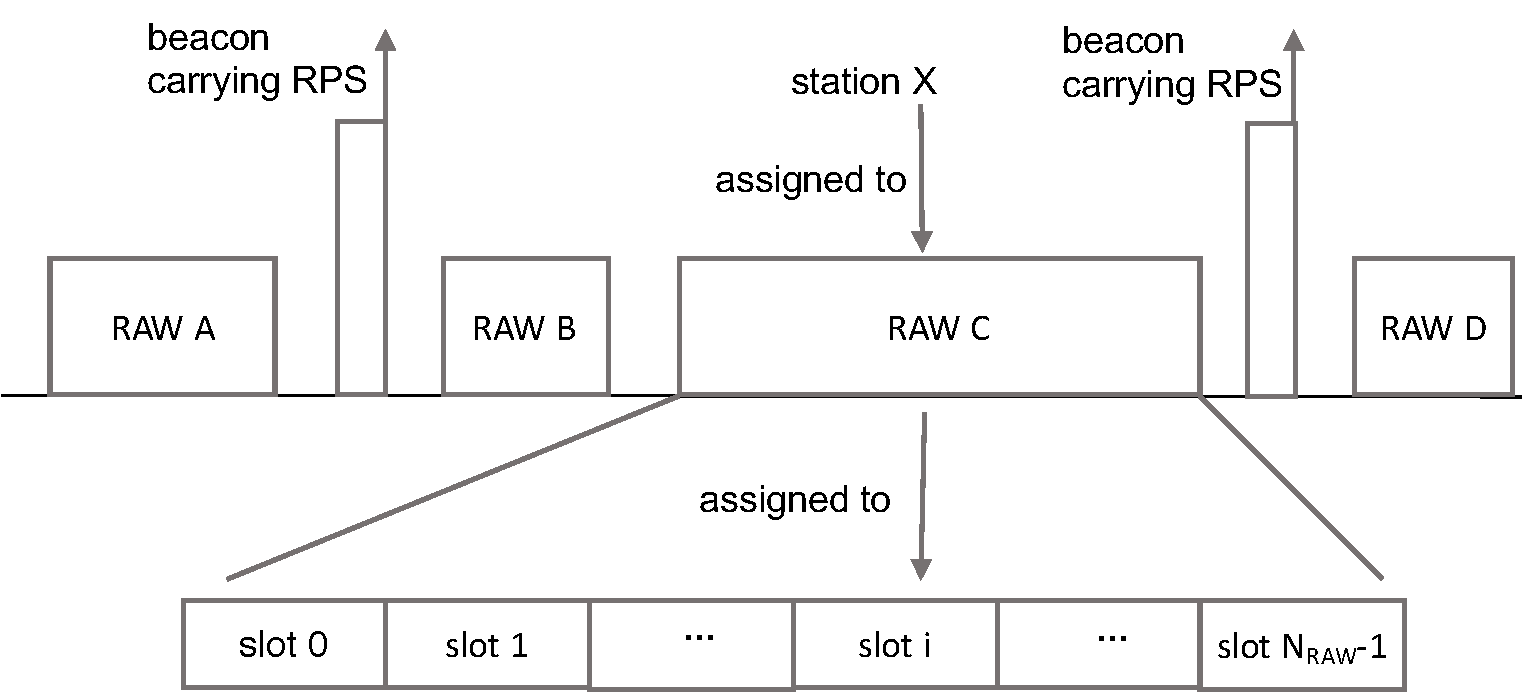
\includegraphics[width=0.8\columnwidth]{figures/raw}
  \caption{Schematic representation of the \gls{raw} mechanism.\label{fig:RAW}}
\end{figure}

%The proposed \gls{raw} feature in 802.11ah aims to reduce collisions and improve performance in dense \gls{iot} network where hundreds or even thousands of stations are simultaneously contending for channel access. It restricts the number of stations that can simultaneously access the channel by splitting them into groups and only allowing stations that belong to a certain group to access the channel at specific times.

Figure \ref{fig:RAW} schematically depicts how RAW works. Specifically, the airtime is split into intervals, some of which are assigned to RAW groups, while the others are considered as shared channel airtime and can be accessed by all stations. Each interval assigned to a RAW group is preceded by a beacon that carries a \gls{rps} information element that specifies the stations that belong to the group, as
well as the interval start time. Moreover, each RAW interval(group) consists of one or more slots, over which the stations in the RAW group are split evenly (using round robin assignment). Therefore, the \gls{raw} related parameters include
 \textit{ number of station assigned to the \gls{raw} groups, number of \gls{raw} groups, duration of each \gls{raw} group}, and  \textit{slot number in each \gls{raw} group}. For a more in-depth description of \gls{raw} and IEEE~802.11ah, the reader is referred to existing literature~\cite{80211ahStd, Khorov2015a, sensors80211ah}.
 %Sensor2017

% Figure~\ref{fig:RAW} schematically depicts how \gls{raw} works. Specifically, the channel airtime is split into several intervals, some of which are assigned to RAW groups, while others are shared and can be accessed by all stations using the traditional 802.11 \gls{edca}, which rely on \gls{csma} channel access. At fixed intervals a beacon frame is transmitted, carrying a \gls{rps} information element. The \gls{rps} specifies the stations belonging to each group using the start and end \gls{aid}, the group start time, and duration. Moreover, each RAW group consists of one or more equal-duration slots, among which the stations assigned to the RAW group are evenly split (using round robin assignment). The \gls{rps} information element also contains the number of slots, slot format and slot duration count sub-fields, which jointly determine the RAW slot duration. For a more in-depth description of \gls{raw}, the reader is referred to existing literature~\cite{Khorov2015a,Sensor2017}.

% \begin{figure}[t]
%   \centering
%   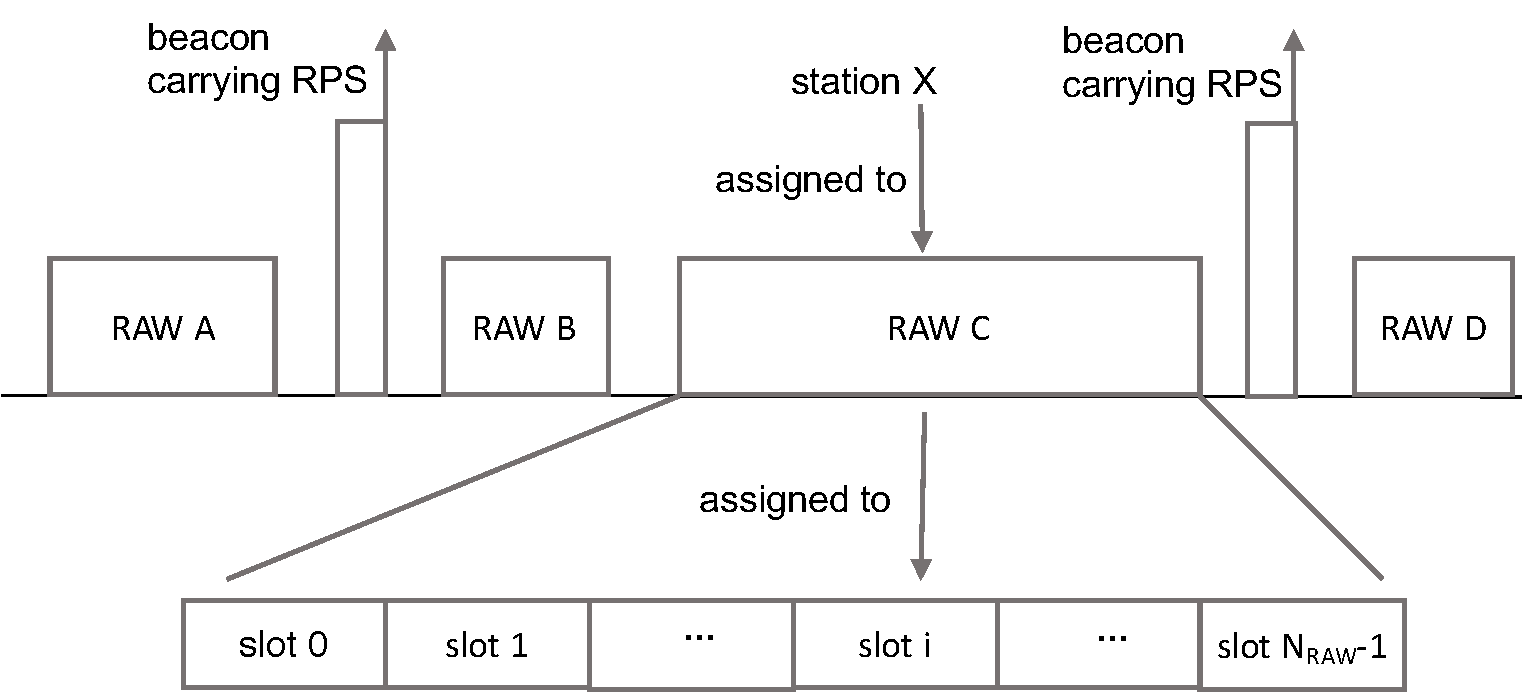
\includegraphics[width=0.8\columnwidth]{figures/raw}
%   \caption{Schematic representation of the \gls{raw} mechanism.\label{fig:RAW}}
% \end{figure}

An intensive evaluation on \gls{raw} has been conducted in ~\cite{WoWMoM2016}. The results demonstrate that, with appropriate \gls{raw} configuration, the \gls{raw} mechanism can provide substantial performance (e.g., throughput, delay and energy consumption) improvement over legacy channel access method \gls{edca}, in particular for highly-loaded dense network scenarios, while the incorrect \gls{raw} configuration severely deteriorate the performance. Moreover, it reveals the optimal \gls{raw} parameters can be affected by a variety of network-related parameters, for instance, the number of stations, traffic patterns, and network load. Therefore, in order to configure the \gls{raw} with the optimal parameters, a model on \gls{raw} is needed to be able to predict the performance for the given \gls{raw} parameters values and given network conditions. Concretely, the model takes network conditions and a \gls{raw} configuration as input, and predicts one or more performance metrics (e.g., throughput or energy consumption) as output. Although several \gls{raw} models have been proposed, they are either too computationally hard to be used in real-time, or rely on certain simplifications (e.g., no capture effect, no hidden nodes, homogeneous stations, saturated traffic). Such simplifications limits the usages of the \gls{raw} models, making it difficult to apply them to realistic \gls{iot} scenarios.

In this paper, we present a surrogate model on \gls{raw} performance for realistic \gls{iot} scenarios. The model is trained using realistic simulation results (with capture effect enabled and the presence of hidden nodes), and support heterogeneous stations with different MCSs and packet size. Although the \gls{raw} configuration depends on many input variables that leads to a wide range of values, the model can be accurately trained with very few labeled sample data points. Moreover, once trained, evaluating the model is equivalent to a constant-time table lookup, which can be easily executed in real-time. To the best of our knowledge, this is the first \gls{raw} model that support heterogeneous stations with different MCSs and packet size.


The remainder of this paper is structured as follows. Section~\ref{sec:related_work} describes the  related work on \gls{raw} performance modeling and compares them to our contributions.
%Section~\ref{sec:SUMO} details the methodology used to define and train the surrogate model. 
The training of of surrogate \gls{raw} model is described in Section~\ref{sec:modeling}. Section~\ref{sec:evaluation} evaluates the accuracy of our presented model. Finally, Section~\ref{sec:conclusion} offers conclusions and a short overview of future work.


%Several algorithms have been proposed to determine suitable RAW parameters. For sensor network traffic with either 1 packet per station or under saturation, some analytical models were proposed. These models are based on different techniques, such as probability theory~\cite{Wang2015,Raeesi2014a}, Markov chains~\cite{Khorov2015b,Zheng2014}, multi-objective game theory~\cite{Bel2014}, and maximum likelihood estimation~\cite{Park2014b}. However, these models are computationally hard, which makes it infeasible to execute them in real-time on actual AP hardware. As an alternative that is computationally feasible and deployable, several partitioning algorithms were proposed. They partition the stations into different RAW slots based on different metrics, such as arbitration inter-frame space number (AIFSN) value~\cite{Ogawa2013}, and station traffic load ~\cite{Chang2015}. However, this information is not known to the AP in reality, also making them infeasible to implement. Recently, we proposed a real-time station grouping algorithm, named TAROA, by estimating the traffic conditions of each station with information only available at the AP~\cite{Sensor2017}. In contrast to other state-of-the-art algorithms it is capable of adjusting its RAW configuration in real-time, in face of station and traffic dynamics. 
%\section{802.11ah and \gls{raw} \label{subsec:802.11ah} }
%\begin{itemize}
%\item Explanation of 802.11ah: RAW, min and max MCS, adaptive rate control


 
Like the legacy 802.11ah technologies, in physical layer, 802.11ah supports multiple transmission rate represented by \gls{mcs}. As listed in table \ref{tab:wifi-modes},  the number of supported MCS depends on the channel width, for channel width 1 MHz,  MCS 0 $\sim$ MCS 10 are supported with transmission data rate ranging from 150 Kbps to 4 Mbps, and for 2 Mhz, MCS 0 $\sim$ MCS 9 are supported with transmission data rate ranging from 650 Kbps to 7.8 Mbps, more details can be found in \cite{802.11ahStandard}. The stations are allowed to dynamically choose the MCS  for packet transmission to adapt to the conditions of the wireless channel.

% Table I lists data rates and their MCSs
% when GI and NSS are 8 us and 1, respectively for 1 and 2 MHz
% bandwidth.


\begin{table}[t]
\centering
\caption{802.11ah MCSs for 1, 2~MHz, NSS=1, GI=$8~\mu{}s$}
\label{tab:wifi-modes}
\begin{tabular}{ccccc}
\hline
\multirow{2}{*}{\begin{tabular}[c]{@{}c@{}}MCS\\ Index\end{tabular}} & \multirow{2}{*}{Modulation} & \multirow{2}{*}{\begin{tabular}[c]{@{}c@{}}Coding \\ rate\end{tabular}} & \multicolumn{2}{l}{Data rate (Kbps)} \\ \cline{4-5} 
 &  &  & 1 Mhz & 2 Mhz \\ \hline
0 & BPSK & 1/2 & 300 & 650 \\ 
1 & QPSK & 1/2 & 600 & 1300 \\ 
2 & QPSK & 3/4 & 900 & 1950 \\ 
3 & 16-QAM & 1/2 & 1200 & 2600 \\ 
4 & 16-QAM & 3/4 & 1800 & 3900 \\ 
5 & 64-QAM & 2/3 & 2400 & 5200 \\ 
6 & 64-QAM & 3/4 & 2700 & 5850 \\ 
7 & 64-QAM & 5/6 & 3000 & 6500 \\ 
8 & 256-QAM & 3/4 & 3600 & 7800 \\ 
9 & 256-QAM & 5/6 & 4000 & Not valid \\ 
\multirow{2}{*}{10} & \multirow{2}{*}{BPSK} & 1/2 with 2x & \multirow{2}{*}{150} & \multirow{2}{*}{Not valid} \\
 & & repetition & & \\ \hline
\end{tabular}
\end{table}


As the 802.11 standards do not specify the way of adapting transmission rate, some rate control algorithms have been proposed and used on the real devices to select the appropriate MCS for packet transmission to adapt to the network condition during the past years, for example, Arf \cite{arf1997},  Aarf \cite{aarf2004}, Onoe \cite{Onoe} and Minstrel \cite{minstrel}. The main ideal of these algorithms is to adjust the transmission rate based on the frequency of successful and failed transmission accumulated in the past. 


\begin{figure}[t]
  \centering
   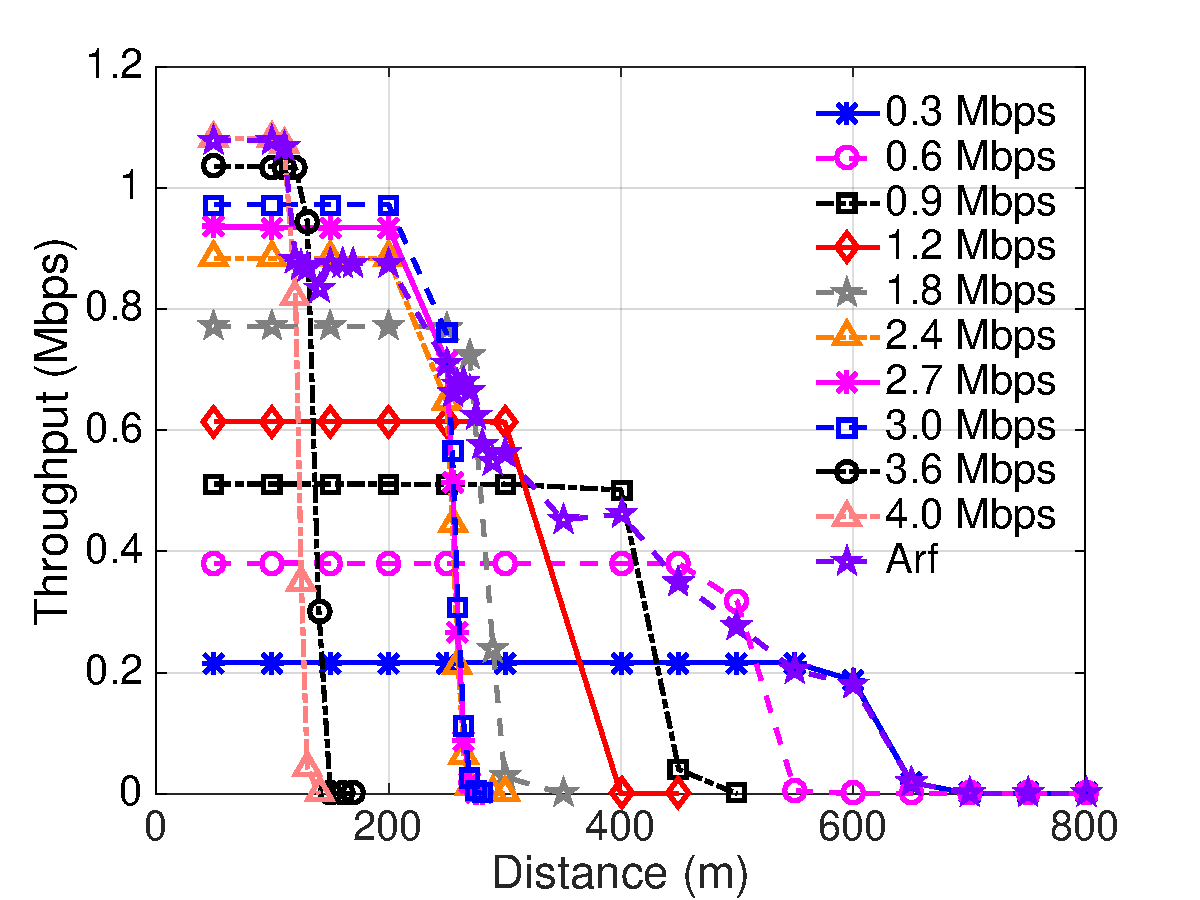
\includegraphics[width=0.45\textwidth]{figures/distance-throughput-512bytes}  \caption{The achievable throughput of each transmission data rate as a function of distance. \label{fig:dist-throughput}}
\end{figure}

\begin{figure}[t]
  \centering
   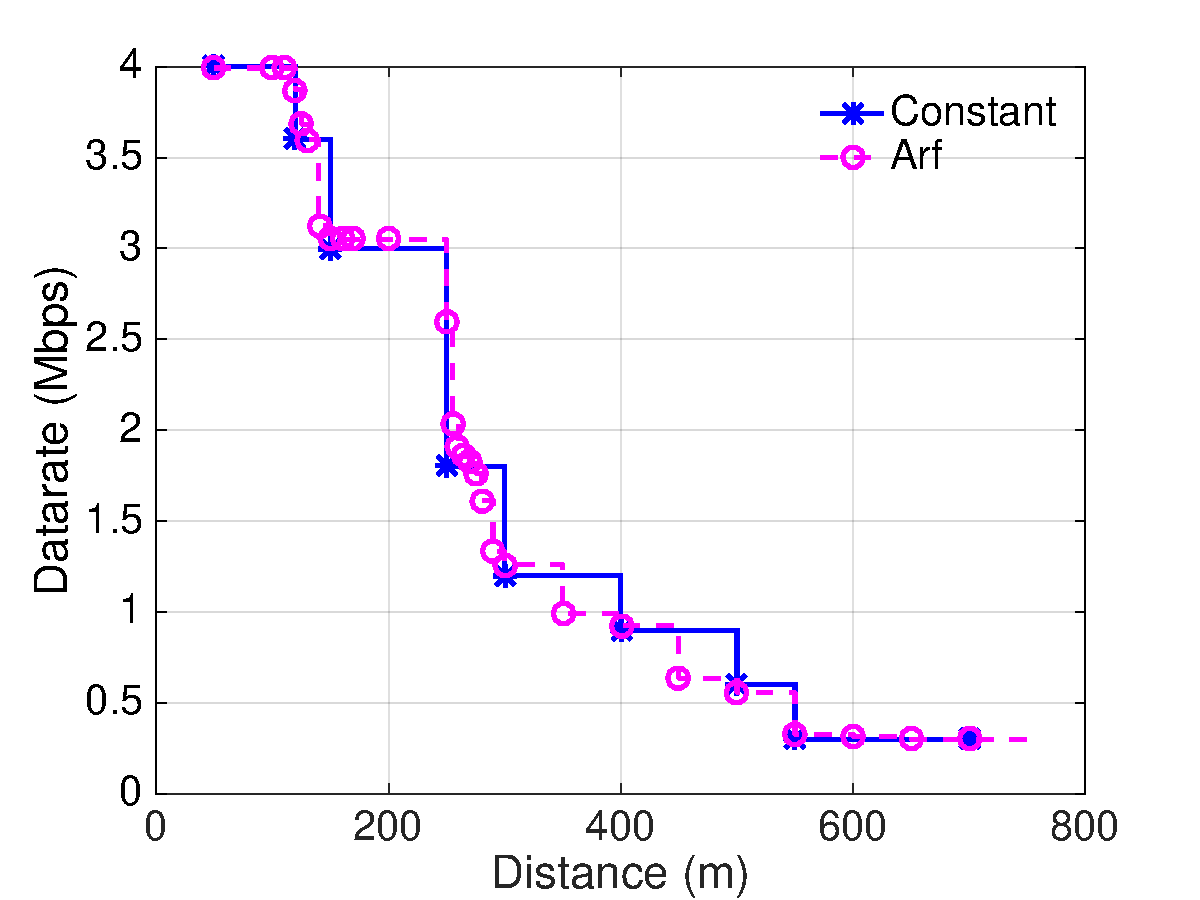
\includegraphics[width=0.45\textwidth]{figures/distance-datarate-512bytes}  \caption{The used transmission data rate for different distance distance. \label{fig:dist-datarate}}
\end{figure}

\textcolor{red}{Explain why not use current rca algorithm for modeling}. For the modeling, we use a simpler rate control method, allowing the stations to select the MCS solely based on its distance to the \gls{ap}, i.e., choosing the MCS which can stably achieve the maximal throughput at a certain distance. Figure \ref{fig:dist-throughput} shows the throughput when a station keeps sending packets (512 bytes) to the \gls{ap} at different distance using a certain transmission data rate, and with Arf algorithm as well. Based on the results, figure \ref{fig:dist-datarate} illustrates the rate control method used in the modeling, showing the selected transmission date rate for a certain distance.
% and the average data rate for a certain distance using arf.
Although the throughput is achieved with packet size 512 bytes, the same results can be achieved by other packet size as well (not depicted).


%Rbar \cite{rbar2001},

% frequency of successful failed transmission accumulated during
% a fixed invocation period of 1000 ms.

% In ARF, each sender attempts to use a higher transmission rate after a fixed number of successful transmissions at a given rate and switches back to a lower rate after 1 or 2 consecutive failures. Aarf is an improved version of Arf, we have chosen to adapt this threshold by using a binary exponential backoff When the transmission of the probing packet fails. Onoe is a credit based ragte control algorithm where the value of the credit is determined by the frequency of successful, erroneous and retransmissions accumulated during
% a fixed invocation period of 1000 ms.

% Minstrel is based solely on acknowledgement feedback. Consequently, estimates of future success probabilities6 at a given rate
% are based only on past success ratios at that rate. With a moderate frequency, frames are selected
% to probe presently unused rates, and feedback from
% those probe frames maintains the probability estimates
% for unused rates so that, should the current best rate
% deteriorate, there is some basis for immediately selecting
% a more successful rate (Section 5.2)8.

% In ns-3, multiple rate control algorithms are available, such as for example \textit{ArfWifiManager}, \textit{ConstantRateWifiManager} and \textit{MinstrelWifiManager}. In the original simulator, the IEEE~802.11ah device could only use these algorithms to adapt the \gls{mcs} within the same channel bandwidth. As IEEE~802.11ah supports multiple channel bandwidths (i.e., 1,2,4,8, and 16~MHz), we modified the \textit{WifiRemoteStationManager} class (the parent class of all the rate control algorithms) to allow automatic switching among different channel bandwidths.

%\item Training methodology (the evaluation scenario used for training)


\section{Background \label{sec:Background}}

 \subsection{IEEE~802.11 ah networks and \gls{raw} \label{subsec:80211ah_raw}}

% \begin{figure}[t]
%   \centering
%   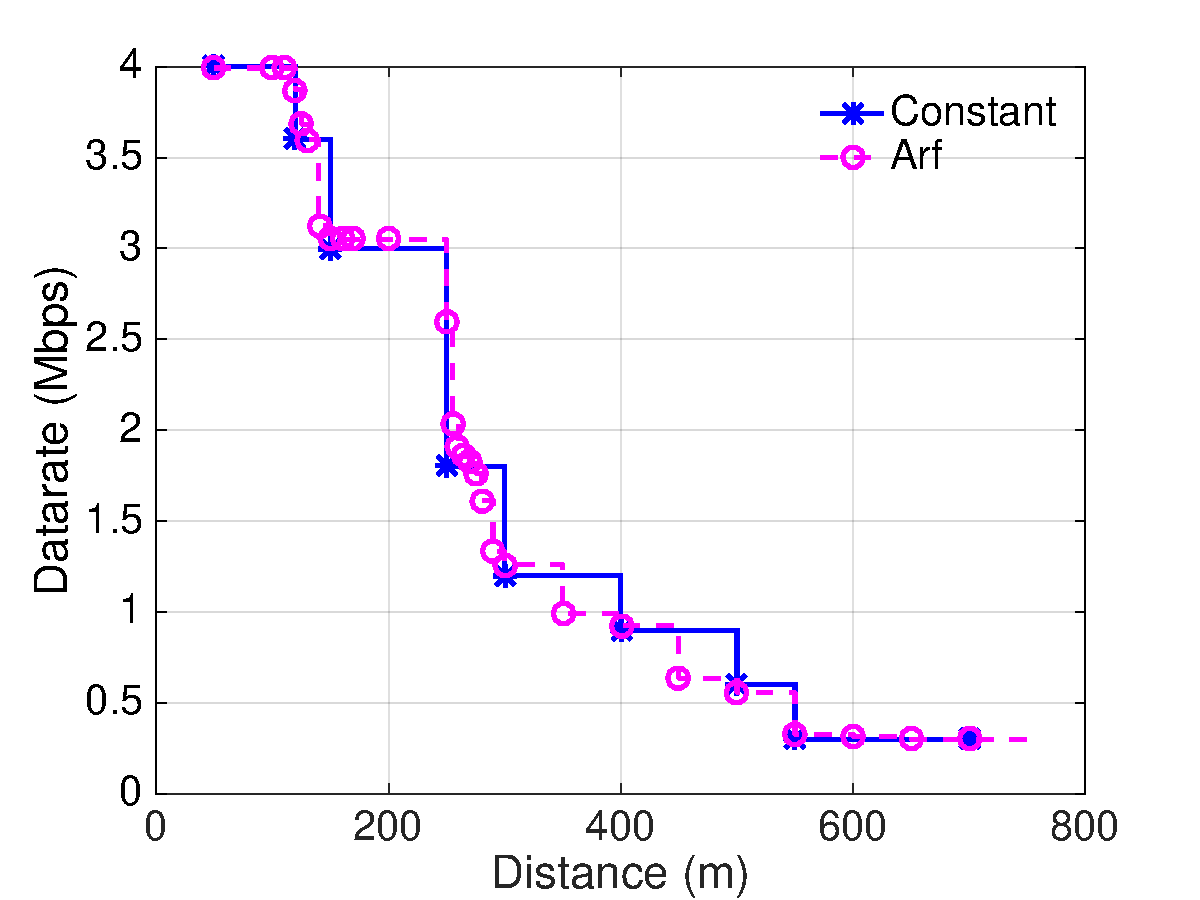
\includegraphics[width=0.45\textwidth]{figures/distance-datarate-512bytes}  \caption{The used transmission data rate for different distance. \label{fig:dist-datarate}}
% \end{figure}


\begin{table}[t]
\centering
\caption{802.11ah MCSs for 1, 2~MHz, NSS=1, GI=$8~\mu{}s$}
\label{tab:wifi-modes}
\begin{tabular}{ccccc}
\hline
\multirow{2}{*}{\begin{tabular}[c]{@{}c@{}}MCS\\ Index\end{tabular}} & \multirow{2}{*}{Modulation} & \multirow{2}{*}{\begin{tabular}[c]{@{}c@{}}Coding \\ rate\end{tabular}} & \multicolumn{2}{l}{Data rate (Kbps)} \\ \cline{4-5} 
 &  &  & 1 Mhz & 2 Mhz \\ \hline
0 & BPSK & 1/2 & 300 & 650 \\ 
1 & QPSK & 1/2 & 600 & 1300 \\ 
2 & QPSK & 3/4 & 900 & 1950 \\ 
3 & 16-QAM & 1/2 & 1200 & 2600 \\ 
4 & 16-QAM & 3/4 & 1800 & 3900 \\ 
5 & 64-QAM & 2/3 & 2400 & 5200 \\ 
6 & 64-QAM & 3/4 & 2700 & 5850 \\ 
7 & 64-QAM & 5/6 & 3000 & 6500 \\ 
8 & 256-QAM & 3/4 & 3600 & 7800 \\ 
9 & 256-QAM & 5/6 & 4000 & Not valid \\ 
\multirow{2}{*}{10} & \multirow{2}{*}{BPSK} & 1/2 with 2x & \multirow{2}{*}{150} & \multirow{2}{*}{Not valid} \\
 & & repetition & & \\ \hline
\end{tabular}
\end{table}

In this section, we provide an overview of the \gls{raw}, the IEEE~802.11ah network environment and its typical settings on the physical and MAC layers. 
%A surrogate \gls{raw} model for such network scenarios is subsequently built to accurately predict the performance.


%simulation environment parameters used during training. 
%Since \gls{raw} is scalable under uplink traffic, 

IEEE~802.11ah mainly targets \gls{iot} network scenarios, where sensors (stations) are randomly placed around the AP within a maximum radius, periodically monitor the environment and send the resulting data to a server (via the \gls{ap}). Like the legacy IEEE~802.11 technologies, at the physical layer, IEEE~802.11ah supports multiple transmission data rates represented by the MCSs. The stations are allowed to dynamically choose the MCS for packet transmission to adapt to the conditions of the wireless channel. As listed in Table \ref{tab:wifi-modes}, the number of supported MCSs depends on the channel width. For channel bandwidth 1 MHz,  MCS 0$-$10 are supported with transmission data rates ranging from 150 Kbps to 4 Mbps, and for 2 Mhz, MCS 0$-$9 are supported with transmission data rates ranging from 650 Kbps to 7.8 Mbps, more details can be found in \cite{80211ahStd}. At every beacon interval, the \gls{ap} broadcasts beacon frame carrying a \gls{rps} information element that specifies the \gls{raw} parameter configurations. Stations retrieve such \gls{raw} information from the beacon frame and access the channel only during their assigned \gls{raw} slot. 
%In order to obtain high performance, there is a need to build a \gls{raw} model that can accurately predict the performance under a variety \gls{raw} parameter values and network conditions.


The \gls{raw} information is carried in the \gls{rps} element, it specifies the stations belonging to the group, the number of slots, slot format and slot duration count sub-fields, which jointly determine the \gls{raw} slot duration as follows \cite{80211ahStd}: 
%\textcolor{red}{\cite{80211ahStd}}: 
\begin{equation} \label{eq:Duration}
D = 500~\mu{}s + C \times 120~\mu{}s  
\end{equation}
where $C$ represents \textit{slot duration count} sub-field, which is either $y = 11$ or $y = 8$ bits long if the slot format sub-field is set to respectively $1$ or $0$. The \textit{number of slots} field is $14-y$ bits long. When $y = 11$, each RAW consists of at most 8 slots and the maximum value of $C$ is $2^{11}-1=2047$, in this case the slot duration is up to $246.14$~ms. Otherwise, each RAW consists of at most 64 slots and the maximum value of $C$ is $2^{8}-1=255$, the slot duration is thus limited to $31.1$~ms. The \gls{raw} group duration is the sum of its slot durations.



% Besides \gls{raw}, there are numerous parameters involved in the physical and MAC layer of IEEE~802.11ah networks.
% %while we mainly focus on the most commonly used scenarios where
% In our experiments, we use the typical parameter settings, 
% as shown in Table~\ref{tab:ns3 parameters}. Given the low-power nature of battery powered sensors, the physical layer parameters are configured based on the low-power 802.11ah radio hardware prototype developed by Ba et al.~\cite{Ba2016}, with a transmission power of 0~dBm, a gain of 0~dBi (for both sensor and \gls{ap}), and noise figure of 6.8~dB. With such physical layer setting, the coverage of the networks is up to 500 meters based on the physical layer performance evaluation in \cite{bellekens2017outdoor}. As the \gls{iot} applications have relatively small payload size, packet size is assumed to be between  32 and 512 bytes.


% For each experimented scenario, we assume a coverage range to be $[d^-, d^+]  \subseteq [0, 500] $  meters and a packet size range to be $[ps^-, ps^+] \subseteq [32, 512] $ bytes. Each station $s$ randomly and uniformly chooses a value $d_s \in [d^-, d^+]$ as its distance to the \gls{ap}, and an integer value $ps_s \in [ps^-, ps^+]$ as its packet size. Based on its distance to the \gls{ap} $d_s$, the station $s$ uses the corresponding MCS for packet transmission according to the rate control method. Several rate control methods have been proposed and used on the real devices for legacy IEEE~802.11 to select the appropriate MCS for packet transmission, for example, Arf \cite{arf1997},  Aarf \cite{aarf2004}, Onoe \cite{Onoe} and Minstrel \cite{minstrel}. For the IEEE~802.11ah network, we use a simpler rate control method, allowing the stations to select the MCS solely based on its distance to the \gls{ap}, i.e., choosing the MCS which can stably achieve the maximal throughput at a certain distance, as shown in Figure \ref{fig:dist-datarate}. The size of the stations' transmit queues is configured to be 10 packets. 
% %For training simplicity, we assume each station sends one packet per second, the built model can be further used by the \gls{raw} optimization algorithms, such as \gls{taora} \cite{Sensor2017,Sensys2017},  to calculate \gls{raw} performance under arbitrary data transmission intervals.



% % As the \gls{iot} applications have relatively small payload size, we limit the packet size range $[\underline{ps}, \bar{ps}] $ to $[32, 512]$,  choose 500 meters as the maximum distance between stations and the \gls{ap} based on the physical layer performance evaluation in \cite{bellekens2017outdoor}.

% %Each experiment runs for 60 seconds of simulated time. As \gls{raw} is configured in each beacon interval of 204.8~ms, the results of every simulated configuration are averaged over 290 beacon intervals, ensuring the generality of the trained model.



% %As the RAW optimization algorithm proposed in Section~\ref{sec:algorithm} groups together stations that use the same \gls{mcs}, the model assumes a fixed \gls{mcs}. However, as \gls{raw} performance depends on the \gls{mcs} used, a different model is to be trained for each \gls{mcs} that stations are expected to use. We illustrate this by developing a separate a high-throughput (HT) and low-throughput (LT) model for two different \gls{mcs} parameter sets. This can be trivially extended to other \gls{mcs} values. 


% \begin{table}[t]
% \centering
% \renewcommand{\arraystretch}{1.2}
% %\tiny
% \caption{\textsc{Simulation parameters used during training}\label{tab:ns3 parameters}}
% \begin{tabular}{ll}
% \hline
% \textbf{PHY parameters}             & \textbf{Value}  \\
% \hline
% %Frequency (Mhz)                      & 868 \\
% TX power (dBm)             & 0    \\
% TX/RX gain (dB)                        & 0     \\
% Noise Figure (dB)               & 6.8      \\  
% %Coding method                  & BCC \\
% Propagation model         & Outdoor \\ %, macro~\cite{Hazmi2012} \\
% Error rate model               & YansErrorRate \\
% \hline
% \textbf{MAC parameters}               & \textbf{Value}  \\
% \hline
% % CWmin                          & 15 \\
% % CWmax                          & 1023      \\
% %Duration of AIFS (us)\textcolor{red}{change to DIFS}            & 316      \\
% Traffic access categories             & \textcolor{black}{ AC\_{BE} } \\
% Duration of AIFS ($\mu$s)             & 264      \\
% Duration of SIFS ($\mu$s)            & 160      \\
% %RTS/CTS                        & not enabled  \\
% Beacon interval (ms)           & 204.8 \\
% %Cross slot boundary            & Enabled \\
% %Rate control algorithm         & constant  \\
% Size of transmission queue (packets)  & 10  \\
% Packet transmission interval (s)        & 1  \\
% Station distribution           & random  \\
% Rate control algorithm                     & XXX \\
% %Average payload size (bytes)           & 64   \\
% %Topology radius (m)     & 200  \\
% \hline
% \end{tabular}
% \end{table}
 
 
\subsection{Related Work \label{subsec:related_work}}


As the IEEE~802.11ah standard does not specify how to configure the actual \gls{raw} grouping parameters, several studies have been conducted on \gls{raw} performance evaluation, modeling and optimization. Raeesi et al. evaluated  \gls{raw} performance using the network simulator OMNeT++, the results demonstrate that the RAW feature provides
substantial performance (i.e., throughput, energy consumption and latency) improvements, in particular in scenarios where there is a relatively high number of collisions and heavily loaded network \cite{Raeesi2014a}. Using an IEEE~802.11ah implementation in ns-3
\cite{WNS32016}, we further evaluated the optimal \gls{raw}  configuration under a variety of network conditions, such as traffic load, number of stations, and traffic distribution among stations~\cite{WoWMoM2016}. These works highlight the impact of network conditions on the optimal \gls{raw} configurations, demonstrate there is a need for a \gls{RAW} performance model, which can predict performance for the given RAW parameter values (e.g., number of groups and slots, group duration, station assignment) and given the current network conditions (e.g., network topology, traffic load, station number). In addition, the \gls{raw} model should be enable to be applicable in real time for \gls{raw} optimization under dynamic network conditions.


%\subsection{\gls{raw} performance models}

%In order to allow the AP to choose the optimal RAW configuration in real-time, a RAW performance model is needed. Given the current network conditions (e.g., network topology, traffic) and a set of RAW parameter values (e.g., number of groups and slots, group duration, station assignment) the model should estimate performance (e.g., in terms of throughput). 

Several mathematical \gls{raw} models have been proposed to calculate  performance under specific network and traffic conditions. These models make use of different techniques, such as probability theory~\cite{Wang2015}, Markov chains~\cite{Raeesi2014a, Khorov2015b,Zheng2014, Evgeny2018, Khorov2015b, Park2014b}, and maximum likelihood estimation~\cite{Park2014b}. Some models  assume stations have infinite packets to send (i.e., saturated model)  \cite{Raeesi2014a, Zheng2014, Park2014b, Evgeny2018}. The works of \cite{Raeesi2014a, Zheng2014, Park2014b} are based on the Bianchi model \cite{bianchi2000performance}, which is a classical mathematical model of the \gls{dcf} for the legacy IEEE~802.11 networks. It utilizes the Markov Chain theory, assumes the network is always in the steady state and saturated mode. Raeesi \textit{et al.}  update the Bianchi model to calculate the probability of collisions inside a \gls{raw} slot without taking into account the finite length of the RAW slot \cite{Raeesi2014a}. Zheng \textit{et al.} extended the Bianchi model to support \gls{raw} considering both cross and non-cross slot boundary traffic, the extended model is able to calculate the throughput with any given number of stations and \gls{raw} duration~\cite{Zheng2014}. Park \textit{et al.} adopt the Bianchi model for the  joint usage of the PS-Poll and RAW mechanisms, and determine the duration of \gls{raw} groups in order to achieve the maximal successful transmission probability for a given number of stations~\cite{Park2014b}. A more accurate mathematical model is recently developed by Lyakhov \textit{et al.} \cite{Evgeny2018}, by taking into account the non-steady state of the backoff function at the beginning of the RAW. Wang \textit{et al.} \cite{Wang2015} , as well as Khorov \cite{Khorov2015b}, proposed none saturated model for low power \gls{iot}, assuming each station sends one packet per \gls{raw} slot interval. By taking into account the reset of the backoff function state at the beginning of the RAW slot, Khorov \textit{et al.} presented a model to calculate the successful packet transmission probability for a certain \gls{raw} group duration~\cite{Khorov2015b}, while Wang's model mainly focus on energy consumption~\cite{Wang2015}. 

The above mathematical models have two main disadvantages. \todo {First of all, these models are computationally hard}. This makes it infeasible to execute them in real-time on actual \gls{ap} hardware, where at most a few milliseconds are available at the start of the beacon interval to calculate a new \gls{raw} configuration. More importantly, they assume certain types of traffic and ideal channel conditions, without communication errors, delays or capture effects. The combination of these factors make such models useful only from a theoretical point of view, to analyze the effectiveness of \gls{raw} under a variety of conditions. However, they cannot be used for real-time station grouping under dynamic and realistic traffic conditions. 
Chang \textitet{et al.} made a step further, to support more diverse traffic demands \cite{Chang2018}. They use the results of two extreme cases (i.e., with infinite traffic and with only a single packet) to extrapolate a regression-based analytical model that can accurately fits the contention success probability of any traffic patterns. However, the regression model does not take the finite length of the RAW slot into account.
 Recently, we proposed a new RAW performance model based on supervised surrogate modeling \cite{wowmom2018}. The model is trained on a limited set of labeled data samples from ns-3 simulation results, support realistic channel conditions, including communication errors, propagation delays and capture effects. However, both of the model of Change \cite{Chang2018} and our previous work \cite{wowmom2018}, only support homogeneous networks (i.e., all stations use the same MCS and average packet size). 

\todo{our contribution}
% Based on the proposed \gls{raw} models, \cite{Chang2018} and \cite{wowmom2018} also developed the \gls{raw} optimization algorithms.  \cite{Chang2018} presents a traffic-aware station grouping algorithm to maximize the \gls{raw} performance. However, due to the drawbacks of the model, the algorithm assumes the number of \gls{raw} groups and \gls{raw} duration are predetermined, which is actually part of the \gls{raw} optimization problem and need to be solved.
% In \cite{wowmom2018}, we present a real-time \gls{raw} optimization algorithm, called \gls{moroa}, supporting a wide range of traffic conditions and heterogeneous stations. However, since the model itself only support stations with same MCS and  packet sizes, the \gls{moroa} only allows same type of stations within a single \gls{raw} group. This limited the flexibility of the algorithm in finding an optimal RAW configuration.




%Moreover, it is very fast to evaluate once trained, allowing it to be used for real-time RAW parameter optimization.




% In addition, a traffic-aware station grouping algorithm was proposed based on the model. However, it assumes the number of \gls{raw} groups and \gls{raw} duration are predetermined, which is actually part of the \gls{raw} optimization problem and need to be solved. The \gls{taroa} algorithm ~\cite{Sensor2017,Sensys2017} can adapt the optimal \gls{raw} parameters in real-time by estimating the current traffic conditions, based solely on information available at the \gls{ap}. However, it derives the optimal number of stations to assign to a group based on saturated state simulation results. Both \cite{Chang2018} and ~\cite{Sensor2017,Sensys2017} only support homogeneous stations (i.e., all stations use the same MCS and average packet size). 

% Recently, we proposed a surrogate model of \gls{raw} which are trained using realistic simulation results, and a real-time \gls{raw} optimization algorithm based on the model, called \gls{moroa}, was proposed supporting a wide range of traffic conditions and heterogeneous stations \cite{wowmom2018}. 
% However, the model itself only support stations with same MCS and  packet sizes, which only allows same type of stations within a single \gls{raw} group, and limited the flexibility of the algorithm in finding an optimal RAW configuration.



%  However, the existing analytical models are computationally expensive and unrealistic due to their assumptions.
 
%  Although a surrogate \gls{raw} model is constructed in \cite{wowmom2018}, it only supports stations with the same \gls{mcs} and packet size, the lack of support on adaptive rate control and diverse packet size make it inapplicable to the realistic scenarios.



%Instead of using Binary Exponential Backoff (BEB) scheme inside of \gls{raw} group, Gopinath \textitet{et al.} proposed a new backoff scheme using an appropriate integer sequences for calculating new Contention Window, and  developed an analytical model  for computing saturated throughput \cite{gopinath2018mathematical}.




% This is not a very realistic assumption for \gls{iot} and \gls{mtc}~\cite{Khorov2015b}. Those models cannot be directly applied to an IoT network, in which each sensor generates traffic periodically. 













% models to estimate the contention success probabilities of the two extreme cases (i.e., with infinite traffic and with only a single packet), and then use the estimates of the two cases to 
















% \subsection{\gls{raw} optimization algorithms}

% In addition to modeling \gls{raw} performance, several algorithms have been proposed to optimize \gls{raw} performance. Some of them group stations based on very simple metrics  \cite{Chang2015, Qutab-Ud-Din2015, Ogawa2013}. Chang \textit{et al.} proposed a set partitioning algorithm that assumes the (static) traffic demand of each station is known by the \gls{ap} and load balances them across groups~\cite{Chang2015}. While stations are grouped based on fully random random AIFSN  ~\cite{Ogawa2013}, or back-off timer value~\cite{Qutab-Ud-Din2015} which is unknown to the \gls{ap} in reality. They all assume the number of \gls{raw} slots and groups is predetermined.






% allowing it to be used for real-time RAW
% parameter optimization.

% by using generic and flexible surrogate models, we present the \gls{moroa}  algorithm, which supports a wide range of traffic conditions and heterogeneous stations.





% This results in significant performance improvements, especially under non-saturated conditions, which are prevalent in \gls{iot} and \gls{mtc} scenarios. 




% However, it still has two shortcomings that can be addressed. First, it derives the optimal number of stations to assign to a group based on saturated state simulation results. Second, it only supports homogeneous stations (i.e., all stations use the same MCS and average packet size). 



% Their simplicity makes it computationally feasible to deploy them in real networks. 

% it is necessary to use this information in real-time, in order to optimize \gls{raw} parameters in an actual network.




% %Several algorithms utilize \gls{raw} to mitigate hidden node collisions by splitting mutually hidden nodes into orthogonal groups~\cite{Yoon2016,Damayanti2016}%{Yoon2016,Dong2016,Damayanti2016}. 





% \cite{Chang2018} 

% Such set partitioning algorithms have several shortcomings. 


% First, high channel contention exists in dense sensor network even without the presence of hidden nodes. Reducing hidden nodes can mitigate collisions to some extent, but is not sufficient. 

% Second, they expect all information, such as the exact traffic intensity of each station, to be readily available at the \gls{ap} side, which in reality is not the case. Third, they assume that the number of groups and slots as well as their duration are predefined, and only the partitioning of stations among them needs to be solved. The number of groups and their duration, however, significantly influence \gls{raw} optimality~\cite{WoWMoM2016}. Finally, none of the presented algorithms take into account traffic dynamics. In a real network, the upstream traffic intensity of stations may change over time for a variety of reasons, and the algorithm should therefore adapt to these changes.

% Recently, we proposed the \gls{taroa}~\cite{Sensor2017,Sensys2017}. It adapts the optimal \gls{raw} parameters in real-time by estimating the current traffic conditions, based solely on information available at the \gls{ap}. However, it still has two shortcomings that can be addressed. First, it derives the optimal number of stations to assign to a group based on saturated state simulation results. Second, it only supports homogeneous stations (i.e., all stations use the same MCS and average packet size). 

% In this paper we present an improved algorithm, called \gls{moroa}, which supports a wide range of traffic conditions and heterogeneous stations, by using generic and flexible surrogate models. This results in significant performance improvements, especially under non-saturated conditions, which are prevalent in \gls{iot} and \gls{mtc} scenarios. 

% %use the simulation results (since the analytic model \cite{Zheng2014} does not support capture effect) of saturated state to derive the optimal number of stations $\sigma^r_\textit{opt}$, while in most case network is not saturated. Second, it can only support homogeneous station, i.e., all station have the same MCS and packet size.


% % In contrast to other state-of-the-art algorithms it is capable of adjusting its \gls{raw} configuration in real-time, in face of station and traffic dynamics. Furthermore, by exploiting the “more data” header field \textcolor{white}{and cross slot boundary} feature, a more accurate traffic estimation technique for IEEE 802.11ah sensor stations was proposed, which is integrated into an enhanced version of the Traffic-Adaptive \gls{raw} Optimization Algorithm, referred to as E-TAROA \cite{Sensys2017}. With more accurate traffic estimation in very dense networks with thousands of sensor stations, E-TAROA results in a significantly more optimal \gls{raw} configuration. Specifically, E-TAROA converges significantly faster and achieves up to 23\% higher throughput and 77\% lower latency than the original TAROA algorithm under high traffic loads.




%\section{Surrogate Modeling \label{sec:SUMO}}

 A surrogate model, is an efficient mathematical model that represents the behavior of a complex system such as a circuit, software or wireless network. A surrogate model is trained at design time, using a limited number of input-output sample data points obtained through simulation or real-life experiments. It is especially suited for tasks with a large input space, as an accurate model can be trained based on relatively little input data points.
 
\begin{figure*}[t]
  \centering
  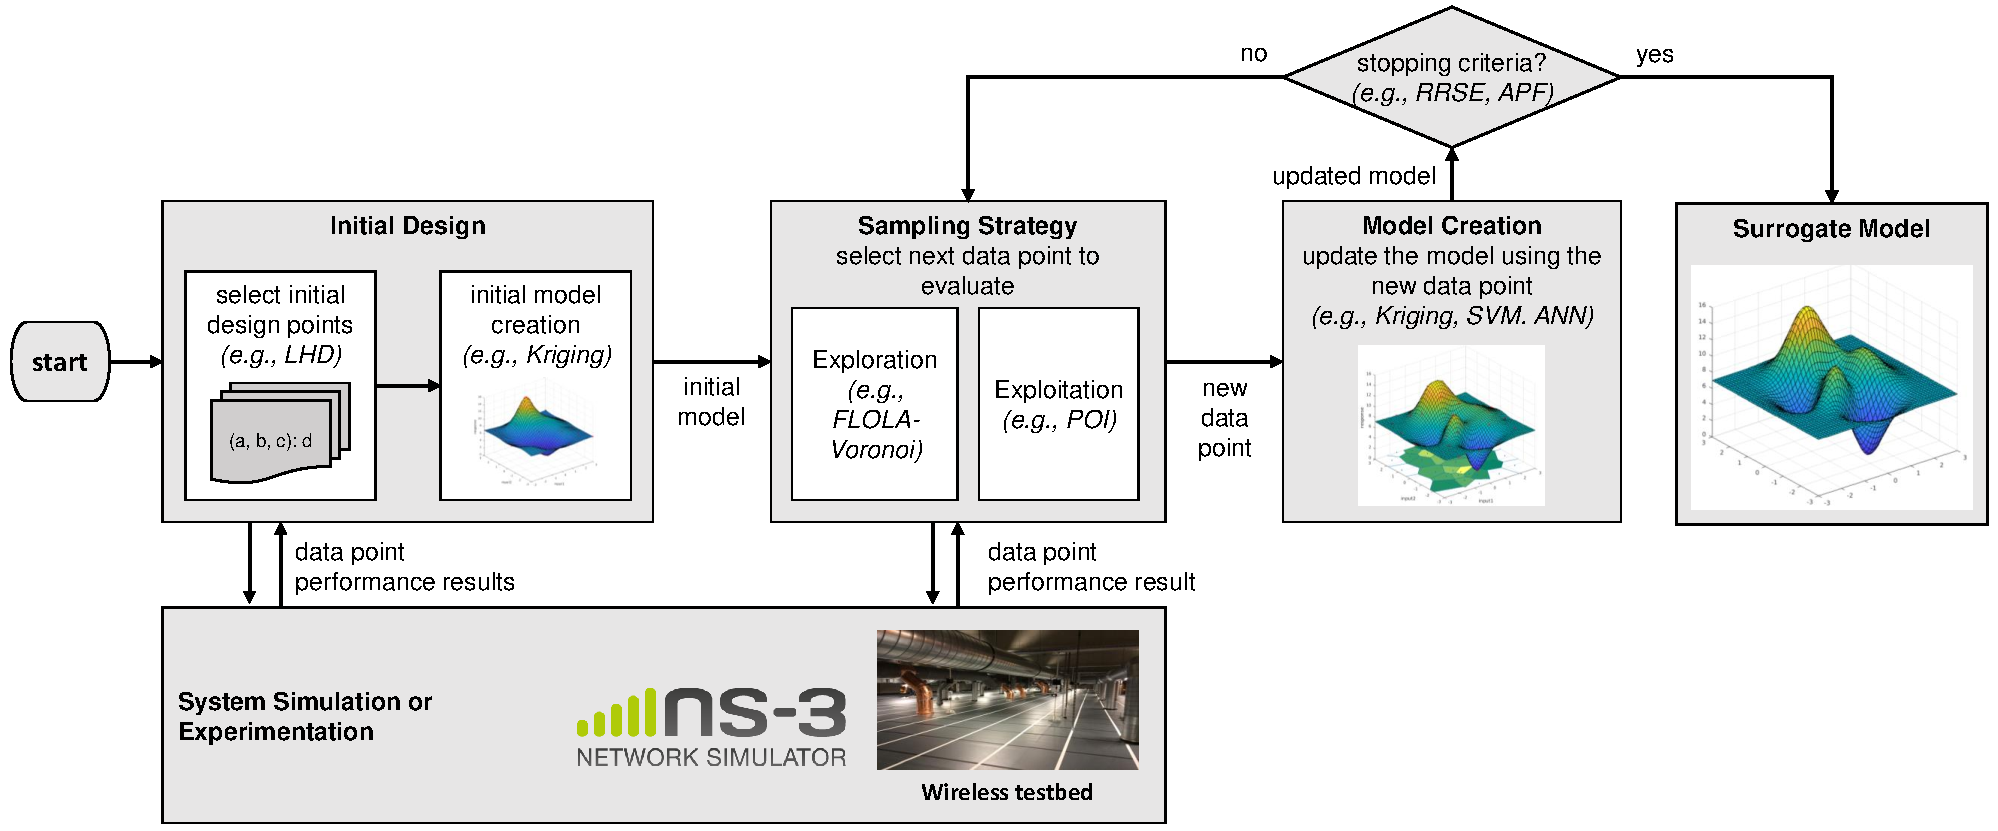
\includegraphics[width=0.9\textwidth]{figures/surrogate_modeling_approach}  \caption{surrogate modeling approach. \label{fig:surrogate_modeling}}
\end{figure*}

%  A simple example of a surrogate model is shown in Figure \ref{fig:sumo}, where the red dots correspond different input configuration settings, and the curve represents the predicted performance over the full design space. The output related to an input data point is generated using either real-life experiments, or via simulation software. 


% Traditionally, the one-shot approach is commonly used to train the model, in which the data points used for training are defined by generating an experimental design based on a space-filling criterion  at once. Because no prior information is available on the behaviour of the response surface it is hard to determine the size of a one-shot design, which is their major downside. 

% Sequential design turns this one-shot approach into an iterative process [3,24]. The acquired data and the constructed models from previous iterations are analyzed in order to intelligently select locations for new data points (sequential sampling). Next, the labels for these additional data points are obtained and new models can be trained or existing models can be updated.


% First of all this means there is no risk of over- or undersampling as the process can be halted when the desired ac- curacy is reached (or if the computational budget is exceeded). A second major advantage is that information provided by the con- secutive labels and intermediate models can guide the selection to obtain optimal locations for new data points. This allows the data distribution to be adapted and refined to the problem at hand as

 
%  Regression models describe the relationship between a response (output) variable, and one or more predictor (input) variables. The responses for new data can be predicted by using the trained model.

 
As illustrated in figure \ref{fig:surrogate_modeling},  surrogate modeling involves the following steps: (i) selecting initial data points to create a first simple model representation (initial design points), (ii) building an initial model with  the the selected initial design points, (iii) selecting the next sample data points to improve the  model if the model accuracy is not satisfactory, otherwise, terminating the modeling process. (iv) building an intermediary model with the previously collected design points, and going back to step (iii). The remainder of this section describes the method used in each steps in details.

 \subsection{Initial Design Points selection}
%However, the initial model requires a set of initial sample points from the design space and performance outputs.

% Before starting the sequential design approach, a coarse initial surrogate model is created based on a small set of data points. 
% To efficiently characterize the system using few design points, ideally space filling designs are used. %Ideally, space filling designs are used to optimally characterize the system behavior. 
% For example, Mehari \textit{et al.} compared several design point selection approaches \cite{SUMOWirelessConferencing}, with the \textit{Latin hypercube design} (LHD) \cite{viana2013} to be generally found the best performing. LHD is a stratified sampling method that selects sample points evenly along the configuration space while ensuring proportional representation of design variables. %Figure \ref{IllustrationSampling}b illustrates a surrogate model based on 20 initial samples using an LHD strategy.

The initial sample points have to be selected carefully to efficiently characterize the system. The existing sampling methods include \gls{lhd} \cite{viana2013}, Orthogonal sampling, Random sampling and  \textit{Hammersley Sequence Sampling} (HSS) \cite{wong1997sampling}. Among them, LHD has the best performance in general is the most commonly used approach, it selects sample points evenly along the configuration space while ensuring proportional representation of design variables. To obtain a better initial model, the number of initial sample points should be large, however, this increase the training time, therefore, a trade-off in terms of the initial design points is normally made. 

\subsection{(Initial) Surrogate Model Creation}

Based on the previously obtained data points, a surrogate model is created to predict how the performance metrics (i.e., output parameters such as throughput, latency or energy consumption) are influenced by the input parameters (i.e. the configuration settings). 

The surrogate model can be created using a variety of supervised machine learning and regression methods, such as Kriging \cite{forrester2008engineering}, polynomial response surfaces, radial basis functions, support vector machines (SVMs), space mapping, or artificial neural networks (ANNs). 


\begin{itemize}
    \item Support vector machines \textcolor{red}{todo}.
    \item  Linear regression, the relationships are modeled using linear predictor functions whose unknown model parameters are estimated from the data. \\
\begin{equation}
y_i = \beta_0 + \sum_{k=1}^{K} \beta_k f_k (X_{i1}, ..., X_{ip}) + \epsilon_i, i = 1, ..., n
\end{equation}
Where $f_k (.)$ is a scalar-valued function of the independent variables, $x_{ij}$,  might be in any form including nonlinear functions or polynomials. The response variable, $y_i$, is a linear function of the coefficients, $\beta_k$. The  noise terms, $\epsilon_i$ ((in contrast with the "signal" provided by the rest of the model)), are uncorrelated, and have independent and identical normal distributions with mean zero and constant variance, $\sigma^2$.
    \item  Gaussian process regression  models, also known as Kriging, are nonparametric kernel-based probabilistic models. A Gaussian prior is assumed for the regression curve, and the errors are assumed to have a multivariate normal distribution and the regression curve is estimated by its posterior mode. The Gaussian prior may depend on unknown hyperparameters, which are usually estimated via empirical Bayes. 
Kriging model are very popular in the modeling of  complex systems, including the complex wireless network \cite{SUMOWirelessConferencing,wowmom2018, LTEoptimization}.The kriging model is formed as:
\begin{equation}
\hat{f} (X) = \sum_{i=1}^{V} {a_i}{k(x, x_i)}
\end{equation}
Where $V$ is the amount of basis vectors, $x$ represent the input data vector and $k(x, x_i)$ is the kernel function. There are several kernel (covariance) functions used by kriging mode, such as, Squared Exponential Kernel, Exponential Kernel, Matern 3/2, Matern 5/2, Rational Quadratic Kernel. Among them, the Matern types of kernel functions are  widely used, and we use the Matern kernenl function with $v=3/2$ and $5/2$ is this paper. 
\end{itemize}

% Regression method: Kriging model, Gaussian Processes model, ... (explain all the ones we evaluate) \\


% ''constant": Model contains only a constant (intercept) term.\\
% ''linear": 	Model contains an intercept and linear terms for each predictor.\\
% "interactions'':	Model contains an intercept, linear terms, and all products of pairs of distinct predictors (no squared terms), considering the relationship among three or more variables, and describes a situation in which the simultaneous influence of two variables on a third is not additive.\\
% ''purequadratic":	 contains an intercept, linear terms, and squared terms.\\
% ''quadratic"	: contains an intercept, linear terms, interactions, and squared terms.\\

% nonparametric regression methods: accommodate more complex regression curves without specifying the relationship between the response and the predictors with a predetermined regression function. Nonparametric regression requires larger sample sizes than regression based on parametric models because the data must supply the model structure as well as the model estimates.



% Based on the **, the regression models can be categorized into several types, including linear regression,
% Gaussian process regression (kriging), regression trees, and support vector machines. 

Each of these methods has its advantages and disadvantages, providing different trade-offs between accuracy and computational complexity. Additionally, in case a priori knowledge is available regarding the most likely behavior, domain specific models can also be applied. However, for many wireless systems, the nature of the true behavior is not known a priori and as such there is no consensus
regarding the best suited or most accurate model. In these cases, often a Kriging surrogate model is used. 

% \cite{forrester2008engineering}. Kriging, also referred to as Gaussian Process Regression,.
% is an interpolation method similar to Inverse Distance
% Weighting (IDW). However, despite its computational
% simplicity, the method also provides confidence intervals
% of each prediction due to the inclusion of the spatial autocorrelation
% of data points [6]. One limitation of Kriging
% models is the inability to model non-continuous behavior.
% In such cases, different models (e.g. neural networks)
% can be used to model the system behavior. However, in
% exchange Kriging models are computationally efficient
% and they provide uncertainty information that can be
% exploited to decide which points should be sampled next.


 \subsection{Sampling strategies}
 
The initial design points explores the configuration space of the system by applying the appropriate design points selection approaches. However, further exploration is needed since the number initial design points is limited, moreover, the initial model may not exploit interesting regions of the system(i.e., non-linear regions).  Therefore, during the sequential design process, at each iteration, the (Root Relative Squared Error (RRSE)  of the currently created surrogate is checked and new sample points is selected if the model accuracy is not satisfactory. 
 
A novel sampling strategy called FLOLA-Voronoi \cite{vanderherten2015} is commonly used to select the next design points to improve the model accuracy.  The FLOLA approach is used for exploiting the non-linear regions, while the Voronoi approach explores the sparsely sampled regions. As the non-linear regions are difficult to model compared to linear regions, more sample points are required in the modeling process. Therefore, the FLOLA approach uses the local linear approximations to estimate the linearity of the region, with the aim of further exploring these regions. For the Voronoi part, a Voronoi tessellation diagram is drawn from tested points and  the area of each Voronoi cell is calculated. A smaller area indicates the presence of nearby explored data points, representing a tightly explored region. A wider area indicates the absence of nearby points, or a sparsely explored region.  Finally, the scores from the the FLOLA and Voronoi are combined to decide the next sample point.



\subsection{Stopping Criteria}

As the goal of the surrogate modeling is to build a model representing the behavior of the complex system using a limited number of experiments, a stop criteria is needed to terminate the modeling process when the intermediary model is accurate enough. Prediction accuracy is calculated by using error measurement metrics (e.g., Root Mean Square Error (RMSE), Root Relative Square Error, Bayesian Estimation Error Quotient, $R^2$) whereby a low error value indicates a good prediction accuracy. 

During the modeling process, the accuracy of model is verified by using cross validation method. At each iteration, the previously obtained samples are divided into training and testing sets, and the predicted response of the model built from the training set is compared against the testing set. The modeling process stops once the cross validation score is below a certain level for a certain number of consecutive iterations. Moreover, the stopping criteria are upper limited to a maximum number of iterations and it will stop execution once the iteration number reaches a specified limit.
%\textcolor{red}{TODO Michael: What is the exact stopping criterion in this case? The metric should stay below a defined threshold for a specific number of subsequent iterations? Please clarify.}





%\item \textit{Surrogate modeling}, or \textit{meta-modeling}, is the methodology that is used to create, analyze and interpret the above models, including selecting and fitting the right meta-models and studying the output and input relationships. %. This includes (i) studying the output and input relationships, (ii) selecting and fitting the right meta-models and (iii) training or creating the models.



% 

\subsection{Matlab Surrogate Modeling (SUMO) Toolbox}

The Matlab Surrogate Modeling (SUMO) Toolbox is a flexible framework for accurate global surrogate modeling \cite{SUMOtoolbox2010}, and can be applied in an autonomous, black-box fashion, or under full manual control. It adopts a microkernel design philosophy with many different plugins available for each step of the surrogate modeling. The behavior of each software component is configurable, and the components can easily be added, removed or replaced by custom implementations. The SUMO Toolbox has already been applied successfully to a very wide range of applications, such as electronic packaging , aerodynamic modeling, process engineering, automotive data modeling, and wireless networks.


% Surrogate modeling provides the answer \cite{SUMOtoolbox2010}. 
% A surrogate model is trained at design
% time, using a limited number of input-output sample data
% points obtained through simulation or real-life experiments.
% Surrogate modeling is especially suited for tasks with a large
% input space, as an accurate model can be trained based on
% relatively little input data points. Moreover, evaluating the
% model at runtime is computationally efficient, equivalent to
% a constant-time table lookup. This makes surrogate modeling
% highly suitable for RAW performance modeling, as the input
% space is very large, and efficient runtime model evaluation is
% needed for real-time RAW parameter selection. Additionally,
% by using realistic simulation results, a surrogate model does not suffer from the same restrictive assumptions as existing
% analytical models.

%Gaussian process regression models also enable you to compute prediction intervals. \\



%The linearity, in the linear regression models, refers to the linearity of the coefficients βk.

%In this paper, several regression models are applied for training the \gls{raw} model.


% \begin{enumerate}
% \item linear regression models
% \item regression trees
% \item Gaussian process regression models
% \item support vector machines
% \end{enumerate}

% \begin{enumerate}
% \item linear regression models
% \item Generalized Linear Models
% \item Nonlinear Regression
% \item Support Vector Machine Regression
% \item Gaussian process regression models (kriging)
% \item Regression Trees
% \end{enumerate}


%The kernel function greatly affect the model accuracy.



%Once you fit a model, you can use it to predict or simulate responses, assess the model fit using hypothesis tests, or use plots to visualize diagnostics, residuals, and interaction effects. stepwise models and mixed-effects models. nonparametric regression methods

\section{Surrogate Model of 802.11ah RAW \label{sec:modeling}}
% \subsection{802.11ah and \gls{raw} \label{subsec:802.11ah} }
% %\begin{itemize}
% %\item Explanation of 802.11ah: RAW, min and max MCS, adaptive rate control

% \begin{figure}[t]
%   \centering
%   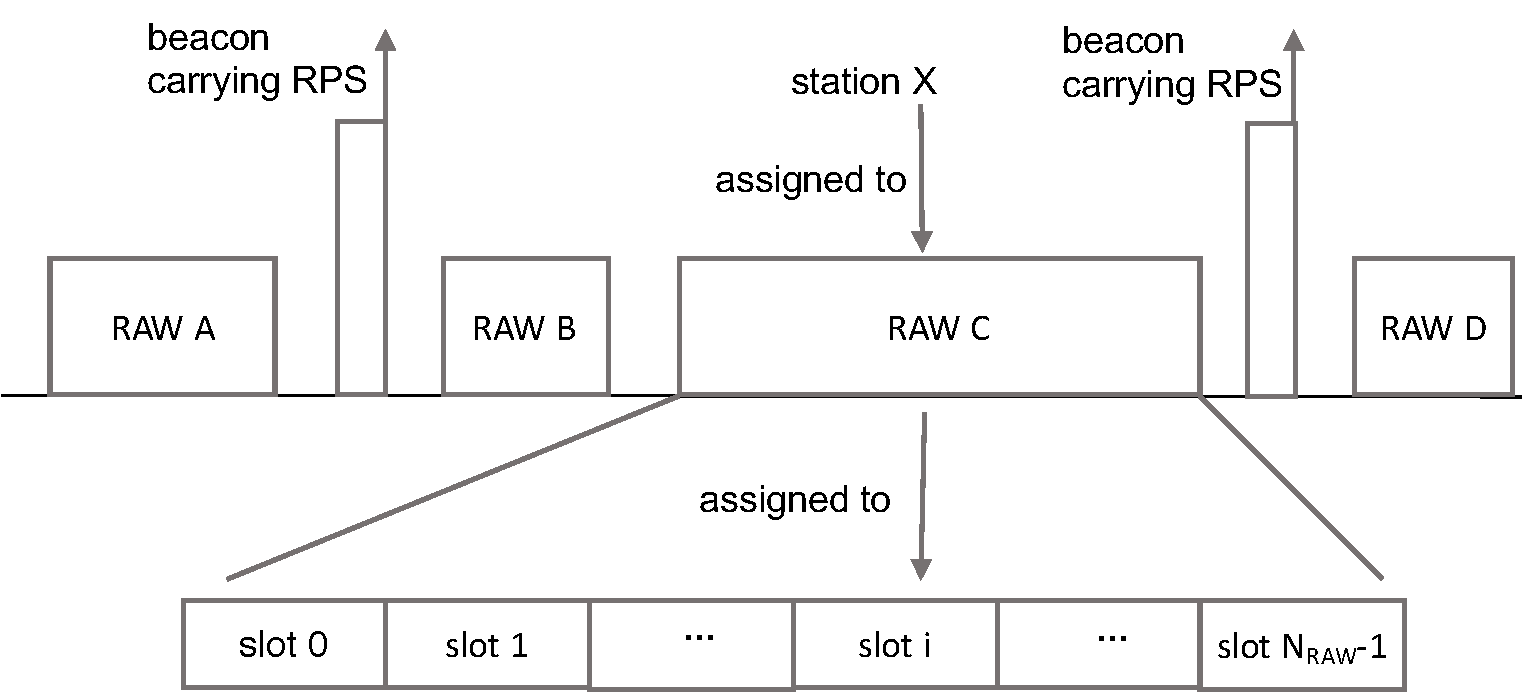
\includegraphics[width=0.8\columnwidth]{figures/raw}
%   \caption{Schematic representation of the \gls{raw} mechanism.\label{fig:RAW}}
% \end{figure}

% The proposed \gls{raw} feature in 802.11ah aims to reduce collisions and improve performance in dense \gls{iot} network
% where hundreds or even thousands of stations are simultaneously contending for channel access.
% It restricts the number of stations that can simultaneously access the channel by splitting them into
% groups and only allowing stations that belong to a certain group to access the channel at specific times.
% Figure \ref{fig:RAW} schematically depicts how RAW works. Specifically, the airtime is split into intervals, some of
% which are assigned to RAW groups, while the others are considered as shared channel airtime and can
% be accessed by all stations. Each interval assigned to a RAW group is preceded by a beacon that carries
% a RAW parameter set (RPS) information element that specifies the stations that belong to the group, as
% well as the interval start time. Moreover, each RAW interval(group) consists of one or more slots, over which
% the stations in the RAW group are split evenly (using round robin assignment). Therefore, the \gls{raw} related parameters include
%  \textit{ number of station assigned to the \gls{raw} groups, number of \gls{raw} groups, duration of each \gls{raw} group}, and  \textit{slot number in each \gls{raw} groups}.
 
% Like the legacy 802.11ah technologies, in physical layer, 802.11ah supports multiple transmission rate represented by \gls{mcs}. As listed in table \ref{tab:wifi-modes},  the number of supported MCS depends on the channel width, for channel width 1 MHz,  MCS 0 $\sim$ MCS 10 are supported with transmission data rate ranging from 150 Kbps to 4 Mbps, and for 2 Mhz, MCS 0 $\sim$ MCS 9 are supported with transmission data rate ranging from 650 Kbps to 7.8 Mbps, more details can be found in \cite{802.11ahStandard}. The stations are allowed to dynamically choose the MCS  for packet transmission to adapt to the conditions of the wireless channel.

% % Table I lists data rates and their MCSs
% % when GI and NSS are 8 us and 1, respectively for 1 and 2 MHz
% % bandwidth.



% As the 802.11 standards do not specify the way of adapting transmission rate, some rate control algorithms have been proposed and used on the real devices to select the appropriate MCS for packet transmission to adapt to the network condition during the past years, for example, Arf \cite{arf1997},  Aarf \cite{aarf2004}, Onoe \cite{Onoe} and Minstrel \cite{minstrel}. The main ideal of these algorithms is to adjust the transmission rate based on the frequency of successful and failed transmission accumulated in the past. 


% \begin{figure}[t]
%   \centering
%   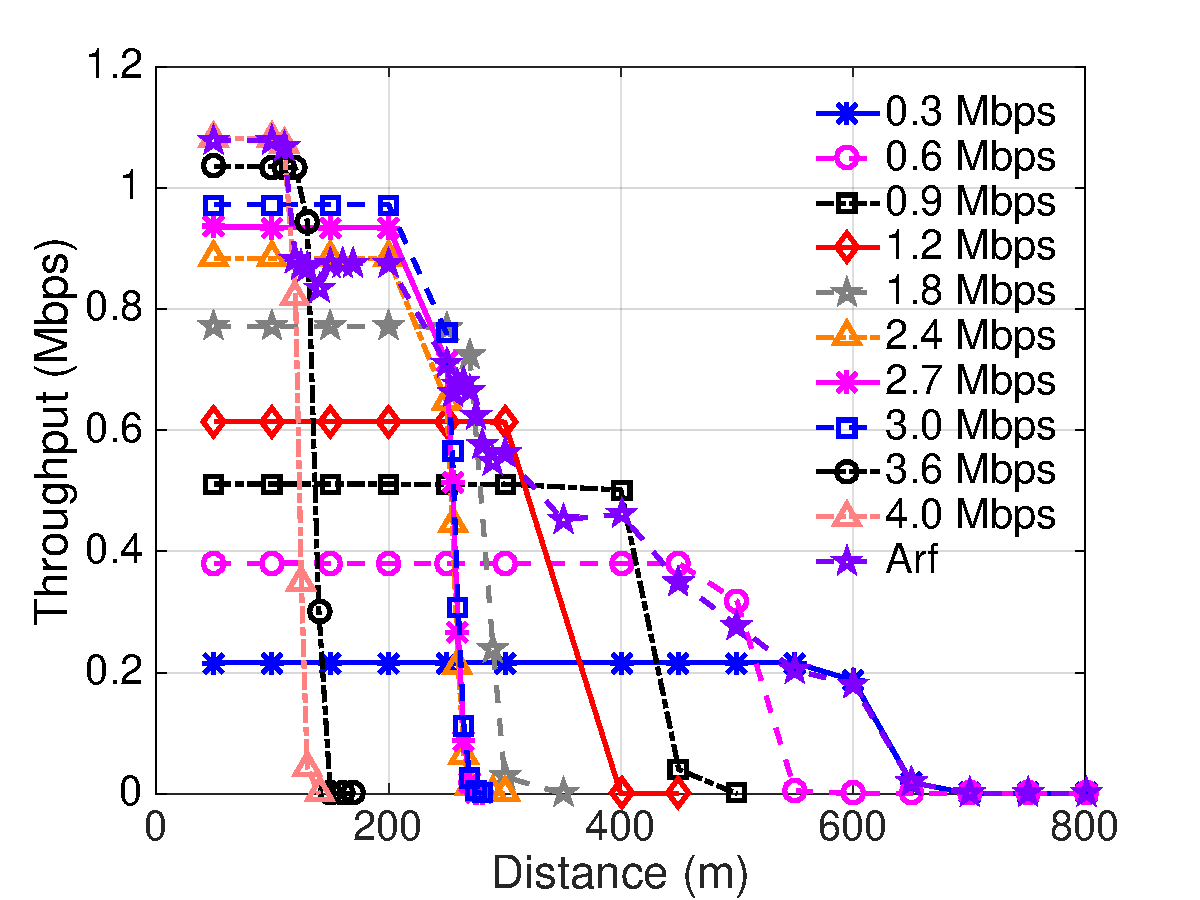
\includegraphics[width=0.45\textwidth]{figures/distance-throughput-512bytes}  \caption{The achievable throughput of each transmission data rate as a function of distance. \label{fig:dist-throughput}}
% \end{figure}

% \begin{figure}[t]
%   \centering
%   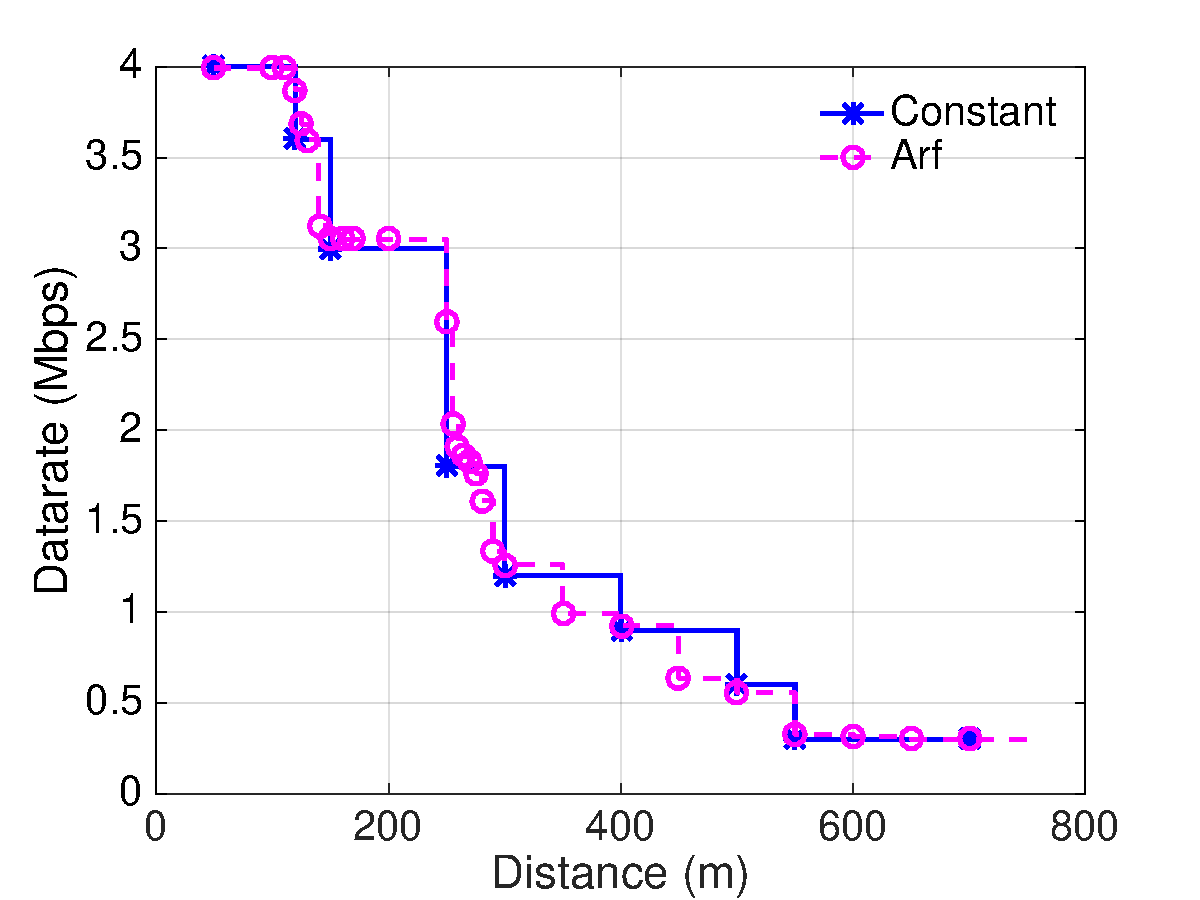
\includegraphics[width=0.45\textwidth]{figures/distance-datarate-512bytes}  \caption{The used transmission data rate for different distance distance. \label{fig:dist-datarate}}
% \end{figure}

% \textcolor{red}{Explain why not use current rca algorithm for modeling}. For the modeling, we use a simpler rate control method, allowing the stations to select the MCS solely based on its distance to the \gls{ap}, i.e., choosing the MCS which can stably achieve the maximal throughput at a certain distance. Figure \ref{fig:dist-throughput} shows the throughput when a station keeps sending packets (512 bytes) to the \gls{ap} at different distance using a certain transmission data rate, and with Arf algorithm as well. Based on the results, figure \ref{fig:dist-datarate} illustrates the rate control method used in the modeling, showing the selected transmission date rate for a certain distance.
% % and the average data rate for a certain distance using arf.
% Although the throughput is achieved with packet size 512 bytes, the same results can be achieved by other packet size as well (not depicted).


% %Rbar \cite{rbar2001},

% % frequency of successful failed transmission accumulated during
% % a fixed invocation period of 1000 ms.

% % In ARF, each sender attempts to use a higher transmission rate after a fixed number of successful transmissions at a given rate and switches back to a lower rate after 1 or 2 consecutive failures. Aarf is an improved version of Arf, we have chosen to adapt this threshold by using a binary exponential backoff When the transmission of the probing packet fails. Onoe is a credit based ragte control algorithm where the value of the credit is determined by the frequency of successful, erroneous and retransmissions accumulated during
% % a fixed invocation period of 1000 ms.

% % Minstrel is based solely on acknowledgement feedback. Consequently, estimates of future success probabilities6 at a given rate
% % are based only on past success ratios at that rate. With a moderate frequency, frames are selected
% % to probe presently unused rates, and feedback from
% % those probe frames maintains the probability estimates
% % for unused rates so that, should the current best rate
% % deteriorate, there is some basis for immediately selecting
% % a more successful rate (Section 5.2)8.

% % In ns-3, multiple rate control algorithms are available, such as for example \textit{ArfWifiManager}, \textit{ConstantRateWifiManager} and \textit{MinstrelWifiManager}. In the original simulator, the IEEE~802.11ah device could only use these algorithms to adapt the \gls{mcs} within the same channel bandwidth. As IEEE~802.11ah supports multiple channel bandwidths (i.e., 1,2,4,8, and 16~MHz), we modified the \textit{WifiRemoteStationManager} class (the parent class of all the rate control algorithms) to allow automatic switching among different channel bandwidths.

% %\item Training methodology (the evaluation scenario used for training)


This section first introduces the surrogate modeling methodology in general, as well as its integration with the ns-3 network simulator. Subsequently, we describe IEEE~802.11ah heterogeneous networks used for training. Furthermore, the input and output parameters of the surrogate \gls{raw} model are designed, and steps of training for  the IEEE~802.11ah heterogeneous networks is described. 


\subsection{Surrogate modeling methodology}


\begin{figure*}[t]
  \centering
  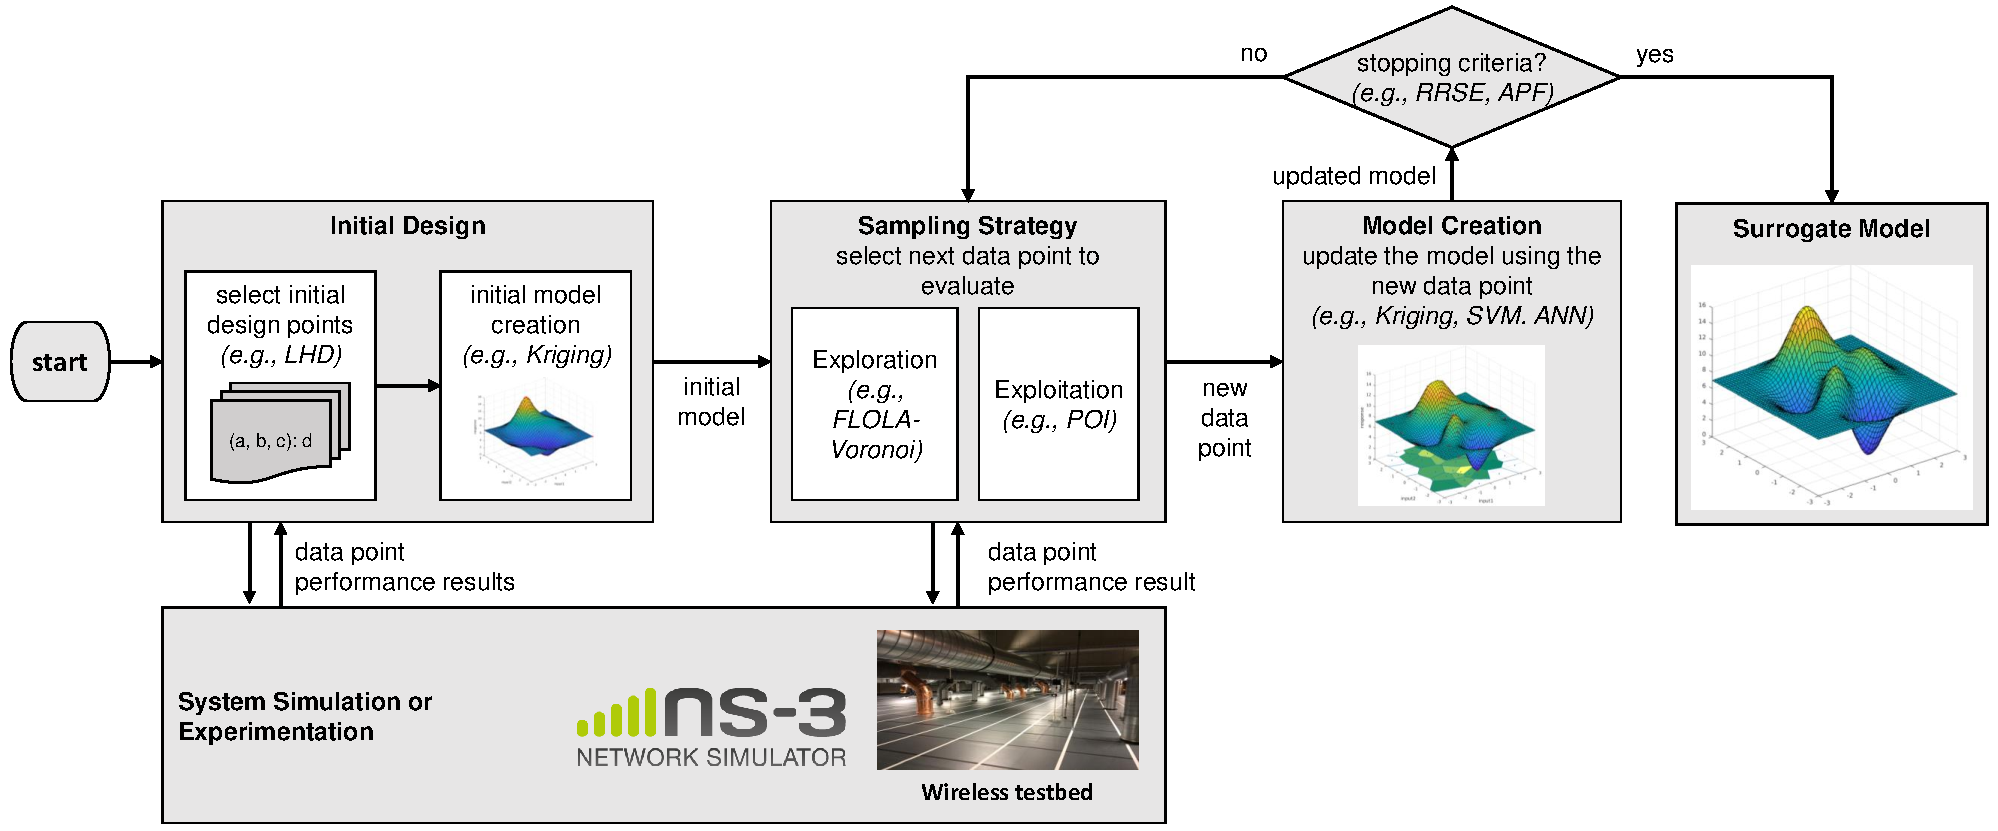
\includegraphics[width=0.75\textwidth]{figures/surrogate_modeling_approach}
  \caption{Surrogate (\gls{raw}) modeling using the ns-3 simulator. \label{fig:sumo-ns3}}
\end{figure*}

 A surrogate model, is an efficient mathematical model that represents the behavior of a complex system such as a circuit, software or wireless network. A surrogate model is trained at design time, using a limited number of input-output sample data points obtained through simulation (e.g., ns-3) or real-life experiments. It is especially suited for tasks with a large input space, as an accurate model can be trained based on relatively few input data points. As illustrated in Figure \ref{fig:sumo-ns3},  surrogate modeling mainly involves four parts.
 \begin{itemize}
 \item  Initial design. Select initial data points as a first simple design space representation, then build an initial model with the selected initial design points by applying supervised machine learning and regression methods. 
 \item  Sampling strategy. Select a few new sample data points to improve the model if the model's accuracy is not satisfactory.  \item  Model creation. Building an intermediary model together with the existing and newly selected design points. 
 \item  Stopping criteria. Define the stopping criteria, stop the training process once the stopping criteria is satisfied, otherwise, select the new sample data points and update the model. 
 \end{itemize}
 
 In this paper, we use the \gls{raw} configurations and network conditions as input, and the obtained performance metric (e.g., throughput) associated with the input values as output. More details are  shown in Section \ref{subs:raw_training}
  
 %the training process section (i.e., section \ref{subs:raw_training})
 


% \subsection{IEEE~802.11 ah networks and \gls{raw} \label{subsec:80211ah_raw}}



% In this section, we provide an overview of the \gls{raw}, the IEEE~802.11ah network environment and its typical settings on the physical and MAC layers. 
% %A surrogate \gls{raw} model for such network scenarios is subsequently built to accurately predict the performance.


% %simulation environment parameters used during training. 
% %Since \gls{raw} is scalable under uplink traffic, 

% IEEE~802.11ah mainly targets \gls{iot} network scenarios, where sensors (stations) are randomly placed around the AP within a maximum radius, periodically monitor the environment and send the resulting data to a server (via the \gls{ap}). Like the legacy IEEE~802.11 technologies, at the physical layer, IEEE~802.11ah supports multiple transmission data rates represented by the MCSs. The stations are allowed to dynamically choose the MCS for packet transmission to adapt to the conditions of the wireless channel. As listed in Table \ref{tab:wifi-modes}, the number of supported MCSs depends on the channel width. For channel bandwidth 1 MHz,  MCS 0$-$10 are supported with transmission data rates ranging from 150 Kbps to 4 Mbps, and for 2 Mhz, MCS 0$-$9 are supported with transmission data rates ranging from 650 Kbps to 7.8 Mbps, more details can be found in \cite{80211ahStd}. At every beacon interval, the \gls{ap} broadcasts beacon frame carrying a \gls{rps} information element that specifies the \gls{raw} parameter configurations. Stations retrieve such \gls{raw} information from the beacon frame and access the channel only during their assigned \gls{raw} slot. 
% %In order to obtain high performance, there is a need to build a \gls{raw} model that can accurately predict the performance under a variety \gls{raw} parameter values and network conditions.


% The \gls{raw} information is carried in the \gls{rps} element, it specifies the stations belonging to the group, the number of slots, slot format and slot duration count sub-fields, which jointly determine the \gls{raw} slot duration as follows \cite{80211ahStd}: 
% %\textcolor{red}{\cite{80211ahStd}}: 
% \begin{equation} \label{eq:Duration}
% D = 500~\mu{}s + C \times 120~\mu{}s  
% \end{equation}
% where $C$ represents \textit{slot duration count} sub-field, which is either $y = 11$ or $y = 8$ bits long if the slot format sub-field is set to respectively $1$ or $0$. The \textit{number of slots} field is $14-y$ bits long. When $y = 11$, each RAW consists of at most 8 slots and the maximum value of $C$ is $2^{11}-1=2047$, in this case the slot duration is up to $246.14$~ms. Otherwise, each RAW consists of at most 64 slots and the maximum value of $C$ is $2^{8}-1=255$, the slot duration is thus limited to $31.1$~ms. The \gls{raw} group duration is the sum of its slot durations.


\subsection{Training scenarios \label{subsec:training scenarios}}


\begin{figure}[t]
  \centering
  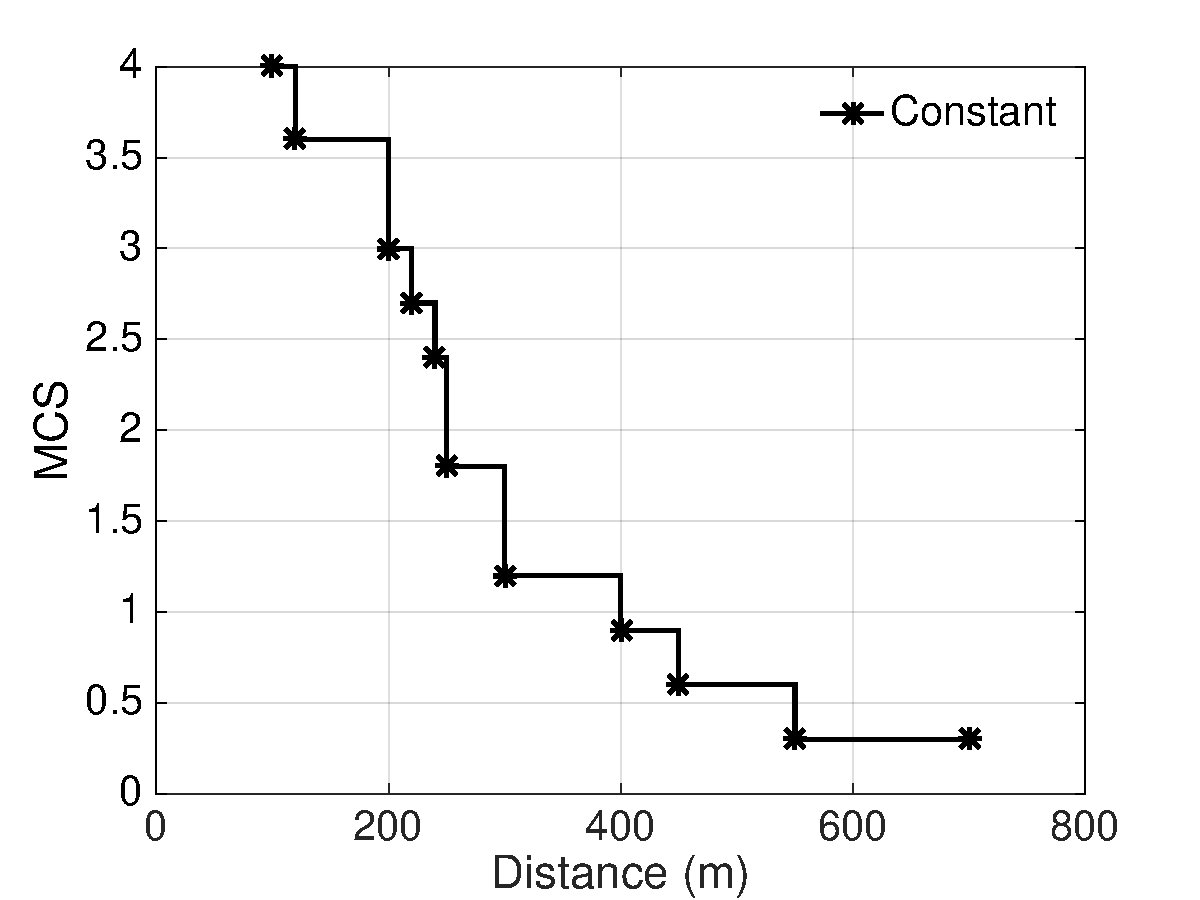
\includegraphics[width=0.45\textwidth]{figures/distance-datarate}  \caption{\gls{mcs} as a function of the distance between a station and \gls{ap}. \label{fig:dist-datarate}}
\end{figure}

% Besides \gls{raw}, there are numerous parameters involved in the physical and MAC layer of IEEE~802.11ah networks.

%while we mainly focus on the most commonly used scenarios where
For the training, we use the typical parameter settings, 
as shown in Table~\ref{tab:ns3 parameters}. Given the low-power nature of battery powered sensors, the physical layer parameters are configured based on the low-power 802.11ah radio hardware prototype developed by Ba et al.~\cite{Ba2016}, with a transmission power of 0~dBm, a gain of 0~dBi (for both sensor and \gls{ap}), and noise figure of 6.8~dB. With such physical layer setting, the coverage of the networks is up to 500 meters based on the physical layer performance evaluation in \cite{bellekens2017outdoor}. As the \gls{iot} applications have relatively small payload size, packet size is assumed to be between 32 and 512 bytes. For each experimented network, we assume a coverage range to be $[d^-, d^+]  \subseteq [0, 500] $  meters and a packet size range to be $[ps^-, ps^+] \subseteq [32, 512] $ bytes. Each station $s$ randomly and uniformly chooses a value $d_s \in [d^-, d^+]$ as its distance to the \gls{ap}, and an integer value $ps_s \in [ps^-, ps^+]$ as its packet size. Based on its distance to the \gls{ap} $d_s$, the station $s$ uses the corresponding MCS for packet transmission according to the rate control method. Several rate control methods have been proposed and used on real devices for legacy IEEE~802.11 to select the appropriate MCS for packet transmission, for example, Arf \cite{arf1997},  Aarf \cite{aarf2004}, Onoe \cite{Onoe} and Minstrel \cite{minstrel2013}. In this paper, We aim to model instantaneous throughput with a single \gls{raw} group (i.e., one beacon interval at most),  \gls{mcs} changes at such a short time slot is are not expected. As such, we allow the stations to select the \gls{mcs} solely based on its distance to the \gls{ap}, i.e., choosing the MCS which can stably achieve the maximal throughput at a certain distance, as shown in Figure \ref{fig:dist-datarate}. The size of the stations' transmit queues is configured to be 10 packets. 
%For training simplicity, we assume each station sends one packet per second, the built model can be further used by the \gls{raw} optimization algorithms, such as \gls{taora} \cite{Sensor2017,Sensys2017},  to calculate \gls{raw} performance under arbitrary data transmission intervals.





% As the \gls{iot} applications have relatively small payload size, we limit the packet size range $[\underline{ps}, \bar{ps}] $ to $[32, 512]$,  choose 500 meters as the maximum distance between stations and the \gls{ap} based on the physical layer performance evaluation in \cite{bellekens2017outdoor}.

%Each experiment runs for 60 seconds of simulated time. As \gls{raw} is configured in each beacon interval of 204.8~ms, the results of every simulated configuration are averaged over 290 beacon intervals, ensuring the generality of the trained model.



%As the RAW optimization algorithm proposed in Section~\ref{sec:algorithm} groups together stations that use the same \gls{mcs}, the model assumes a fixed \gls{mcs}. However, as \gls{raw} performance depends on the \gls{mcs} used, a different model is to be trained for each \gls{mcs} that stations are expected to use. We illustrate this by developing a separate a high-throughput (HT) and low-throughput (LT) model for two different \gls{mcs} parameter sets. This can be trivially extended to other \gls{mcs} values. 


\begin{table}[t]
\centering
\renewcommand{\arraystretch}{1.2}
%\tiny
\caption{\textsc{Simulation parameters used during training}\label{tab:ns3 parameters}}
\begin{tabular}{ll}
\hline
\textbf{PHY parameters}             & \textbf{Value}  \\
\hline
%Frequency (Mhz)                      & 868 \\
TX power (dBm)             & 0    \\
TX/RX gain (dB)                        & 0     \\
Noise Figure (dB)               & 6.8      \\  
%Coding method                  & BCC \\
Propagation model         & Outdoor \\ %, macro~\cite{Hazmi2012} \\
Error rate model               & YansErrorRate \\
\hline
\textbf{MAC parameters}               & \textbf{Value}  \\
\hline
% CWmin                          & 15 \\
% CWmax                          & 1023      \\
%Duration of AIFS (us)\textcolor{red}{change to DIFS}            & 316      \\
Traffic access categories             & \textcolor{black}{ AC\_{BE} } \\
Duration of AIFS ($\mu$s)             & 264      \\
Duration of SIFS ($\mu$s)            & 160      \\
%RTS/CTS                        & not enabled  \\
Beacon interval (ms)           & 204.8 \\
%Cross slot boundary            & Enabled \\
%Rate control algorithm         & constant  \\
Size of transmission queue (packets)  & 10  \\
Packet transmission interval (s)        & 1  \\
Station distribution           & random  \\
%Rate control algorithm                     & XXX \\
%Average payload size (bytes)           & 64   \\
%Topology radius (m)     & 200  \\
\hline
\end{tabular}
\end{table}
 
 
 
\subsection{Parameter design for surrogate \gls{raw} modelling \label{subsec:para_design}}

%\item Input parameters (and motivation and experiments that led to this choice): minimum, maximum, step size, list of parameters, ...
% \begin{itemize}
% \item Add figure(s) to illustrate decisions (cf. Figure Le made in the beginning of the internship)
% \item Average transmission time
% \item RAW parameters.
% \end{itemize}

\begin{figure}[t]
  \centering
  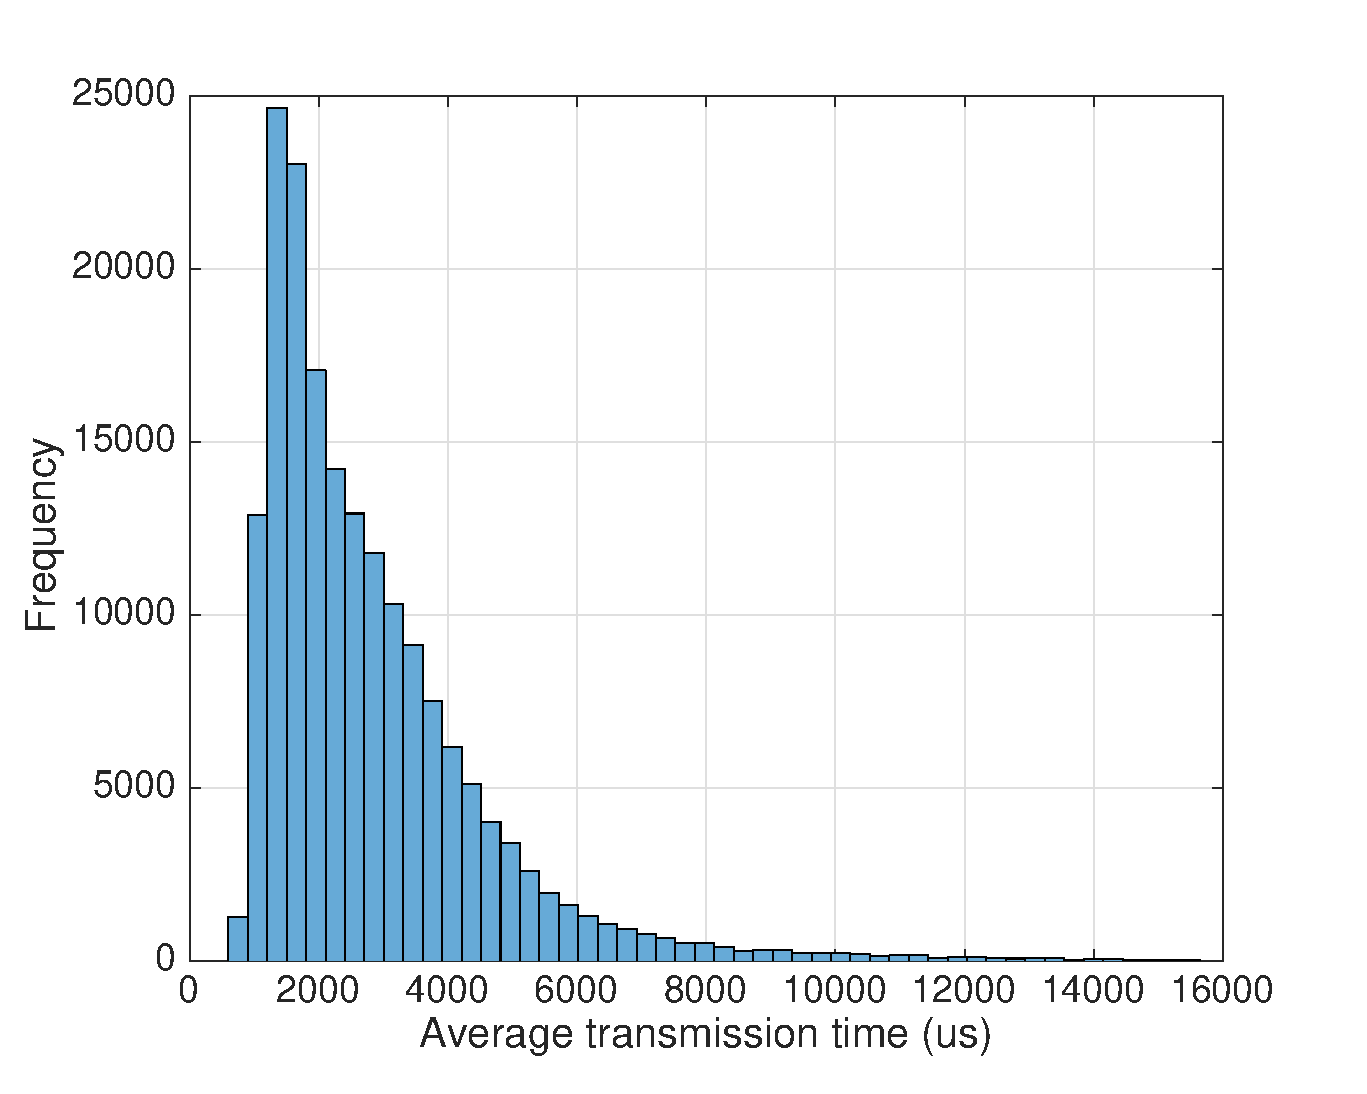
\includegraphics[width=0.75\columnwidth]{figures/histTx}
  \caption{Distribution of average transmission time of 802.11ah networks supporting different coverage and packet size ranges. \label{fig:tx-hist}}
\end{figure}

The goal is to build a surrogate model with a limited number of sample input-output data points, which can accurately predict the performance of a heterogeneous 802.11ah network for a given \gls{raw} configuration and network condition. The input of a data point consists of a set of parameters of a heterogeneous 802.11ah network, and the performance (e.g., throughput) of the associated network is considered as output of the data point. Therefore, a set of parameters should be defined to represent the network conditions and its \gls{raw} configuration. Moreover, the input parameter space needs to be defined, which consists of the minimum and maximum value of each parameter, as well as a step size. The size of input parameters space represents the number of data points of the surrogate model. Among these points, a few of them are sequentially selected as sample data points to train the surrogate model, in order to accurately predict the output of the other data points. Therefore, the parameters and their step sizes should be well chosen, leveraging the trade-off between accuracy and training speed. On the one hand, a small number of parameters and large step sizes lead to a small design space, which needs less training time but poorly characterizes the system. On the other hand, a large number of parameters and small step sizes result in a big design space, which can more accurately characterize the system but needs more training time. As for the output parameter of the model, it should be able to represent the performance metrics (e.g., throughput, energy consumption and latency) with the given input parameters. To simplify the explanation, we focus on throughput as an output metric.


\begin{table}[t]
\centering
\renewcommand{\arraystretch}{1.2}
%\tiny
\caption{\textsc{Definition of the input parameter space}\label{tab:sumo parameters}}
\begin{tabular}{llll}
\hline
\textbf{Parameter}       & \textbf{Min}  & \textbf{Step}   & \textbf{Max}  \\
\hline
$n_r$        & 60 & 5 & 400  \\
$d_r$ ($\mu$s)          & 40960 & 5120 & 204800    \\
$s_r$           & 1 & 5 & 50    \\
$\hat{t}_p$ ($\mu$s)           & 1000 & 250 & 5000    \\
\hline
\end{tabular}
\end{table}



\subsubsection{\gls{raw} parameter design \label{subsec:raw_para_design}}

As mentioned in Section \ref{subsec:80211ah_raw}, the related parameters of a \gls{raw} group $r$ are, number of station assigned to the \gls{raw} groups $n_r$, duration of the \gls{raw} group $d_r$, and slot number in the \gls{raw} group $s_r$. In our previous work \cite{wowmom2018}, we selected the appropriate range and step size for each \gls{raw} parameter, which leads to high model accuracy and only a limited number of training data points. Therefore, in this paper, we use the same \gls{raw} parameter values. A minimum value of $60$ and maximum value of $400$ stations per group $n_r$ were deemed to cover all possible traffic conditions, $d_r$ is varied between $40960$~$\mu$s and $204800$~$\mu$s, and  $s_r$ is between 1 and 50. This results in $2.3 \times 10^7$ possible combinations, which is too high to train the model in a feasible amount of time. Thus, a good step
size for each of the three \gls{raw} parameters is chosen, leveraging the trade-off between accuracy and training speed.
For $n_r$ and $s_r$ a step size of 5 was selected, and $s_r$ takes on values from the set $\left\{1, 5, 10, ..., 50\right\}$. As such, $25047$ combinations are generated with \gls{raw} parameters, and the total number of data points of the input space is $25047 \times m$, where $m$ represents the number of combinations from the network condition parameters.

\subsubsection{Network condition parameter design \label{subsec:network_para_design}}

As in the IEEE~802.11ah network environment, the typical settings are used for  some parameters (cf. Table \ref{tab:ns3 parameters}), the remaining variables are the  packet size  range $[ps^-, ps^+]$ and coverage range $[d^-, d^+]$, which leads to a variety of heterogeneous networks. It seems straightforward to use these four parameters as the input parameters of model, representing the networks conditions. However, this would result in a huge input design space, significantly increasing the required training data points and therefore slowing the training speed. According to the training scenarios, the $d^-$ and $d^+$ is between 0 and 500 meters with $d^- \leq d^+$, the $ps^-$ and $ps^+$ is between 0 and 512 bytes with $ps^- \leq ps^+$. With step size 1, the coverage range and packet size range  results in 125751 and 115921 combinations respectively, and $m = 1.4 \times 10^{10} $ combinations in total. Therefore, the total number of data points of the input space is $25047 \times m = 3.5 \times  10^{14}$. With a large step size, for instance, 100 for  the coverage and 120 for the packet size, the input space still has $7.89 \times  10^{6}$ data points. Both cases results in design space that is too big to achieve feasible convergence. Therefore, as MCS (equivalent to data rate and derived from distance) and packet size can jointly determine the transmission time of a packet, we decide to use average packet transmission time $T_x$ of all stations as the input parameter representing network conditions, leveraging the trade-off between accuracy and training speed (equivalent to input design space). The remaining of this section elaborates the highly reduced input design space, including the distribution of average transmission time $T_x$ among different IEEE~80.211ah network scenarios, and its minimum,  maximum and step values. The accuracy is detailed in Section \ref{subsubsec:txselection}.

%and packet receiving rate as the output parameter of the mode. 
%The reason is detailed in the reminder of this section.

%Hereby we present the distribution of average transmission time $\hat{t}_p$ among the IEEE~80.211ah network scenarios, and define its minimum and maximum value as an input parameter of the surrogate model. 
Figure \ref{fig:tx-hist} depicts the distribution of average transmission time $T_x$ of the training scenarios. The figure is derived from the simulation results of a broad range of networks which have different coverage and packet size ranges. The $d^-$ and $d^+$ parameters are selected from [\textit{min}:\textit{step}:\textit{max}]=[0:10:500] meters, and the $ps^-$ and $ps^+$ belong to  [\textit{min}:\textit{step}:\textit{max}]=[32:32:512] bytes. Therefore, the combination of coverage and packet size range leads to 180336 different 802.11ah networks. We calculate the average packet transmission time across all stations in each network, and count how many times a certain average transmission time occurs among the 180336 802.11ah networks. The results in Figure \ref{fig:tx-hist} shows the average transmission time in the range of [1200 1500] $\mu$s occurs the most (24660 times),  and the average transmission time is mainly between 1000 and 5000 $\mu$ (around 90\% of all experiments). Therefore,  when average transmission time is considered as an input parameter of the model, 1000 and 5000 $\mu$s can be used as its minimum and maximum value for the training. A step size of 250 is selected, leading to $m = 17$ different values for average transmission time.
Therefore, using average transmission time results in a design space with only $25047 \times m = 425799$ data points, from which samples are drawn during the training.
It is only $1.2 \times 10^{-7} \%$ of all data points (i.e., $3.5 \times 10^{14}$) in the design space in which $d^-$, $d^+$, $ps^-$ and $ps^+$ are used as input parameters to represent the network.

% much less than $3.5 \times 10^{14}$ data points caused by using $d^-$, $d^+$, $ps^-$ and $ps^+$ as input parameters to represent the network.
%\textcolor{red}{The surrogate model can interpolate the results for data points outside the input parameter space}.


%Results for data points outside the input parameter space are obtained via linear interpolation of the two nearest data points included in the model.
 
 %\textcolor{red}{todo, explain the huge space caused by the four parameters.}

%%[0, 500], [32, 512]
%%step size 1
%% for [0, 500], num = 501 + 500 + ... + 1 = 125751
%% for [32, 512], num = 481 + 480 + ... + 1 = 115921
%% total, 125751 * 115921 = 14577181671
%% with raw, total, 14577181671 * 25047 = 365114669313537

%% step size 100/120
%% for [0, 500], 21
%% for [32, 512], 15
%% total, 315
%% with raw, total, 315 * 25047 = 7889805
 \subsubsection{Output parameter design \label{subsec:output_para_design}}

 As an average transmission time can consist of a variety of packet size ranges that can affect the throughput, the successfully packet receiving rate (i.e., number of received packets per seconds) is used as the metric of performance. The throughput can be subsequently calculated
together with the packet size range for a specific network scenario.
 

 
 
% As small average transmission time, for example transmission time $1000$ \textit{us}, has relative short distance  and packet size, leading to small variance on the packet rate. While for large transmission time, stations have longer distance to the \gls{ap} and larger packet size, therefore, the packet rate has larger variance.

% with average transmission time no more than 3000 us have the similar performance regardless of the coverage and packet size range. However, with larger average transmission time, the results are quite different,  in this case, the average transmission time can not be used to represent the network, and therefore, can not be used as an input parameter to train the model. As such, we limit the average transmission time to between 1000 us and 3000 us. We choose 250 as the step size of  $\hat{t}_p$.



% In probability theory and statistics, the coefficient of variation (CV), also known as relative standard deviation (RSD), is a standardized measure of dispersion of a probability distribution or frequency distribution.



Therefore, the surrogate model can be represented as a function  $\mathcal{F}$ :
\begin{equation} \label{eq:raw_model}
p_r = \mathcal{F}(n_r, d_r, s_r, T_x) 
\end{equation}
Where $p_r$ represents the packet receiving rate. It aims to predict the performance of a heterogeneous 802.11ah network with average packet transmission time $T_x$, for a given RAW group $r$ with duration $d_r$, consisting of $s_r$ slots, and with $n_r$ stations assigned to it. The definition of the input parameters are listed in Table \ref{tab:sumo parameters}.







%\subsection{The selection of parameter average packet transmission time \label{subsubsec:txselection}}



\subsection{Network condition parameter analysis \label{subsubsec:txselection}}

In this section, we demonstrate that the average transmission time 
%and packet receiving rate 
is a proper input parameter for the model, as it can accurately represent the network conditions with highly reduced design space size. As the size of design space has been discussed in section \ref{subsec:network_para_design}, this section focus on the accurate representativeness. The accurate representativeness lies on that, networks with the same average transmission time have small variance in the behaviour, i.e., similar packet receiving rate, in order to accurately predict one for the other. Since the model is mainly used for optimization, we are more interested in the large values and high \gls{pdr}.
\gls{pdr} is defined as the ratio between the number sent packets, and number of received packets predicated by the model. The large values signify higher throughput and better performance, and high \gls{pdr} indicates lower packet loss. The \gls{cov}, also known as relative standard deviation, is a measure of variation or dispersion of a set of data values. It is calculated by dividing the standard deviation of a series of values by the average of the values. In this section, the \gls{cov} is used as the criterion to evaluate the variance of the output (i.e., packet receiving rate)  of networks with the same average transmission time $T_x$ but different coverage and packet size ranges. As Figure \ref{fig:tx-hist} shows, there are a large number of coverage and packet size ranges that can lead to the same average transmission time. 


\begin{figure*}[t]
    \centering
    \subfloat[All data points  \label{fig:tx-diff-Prate-all}]{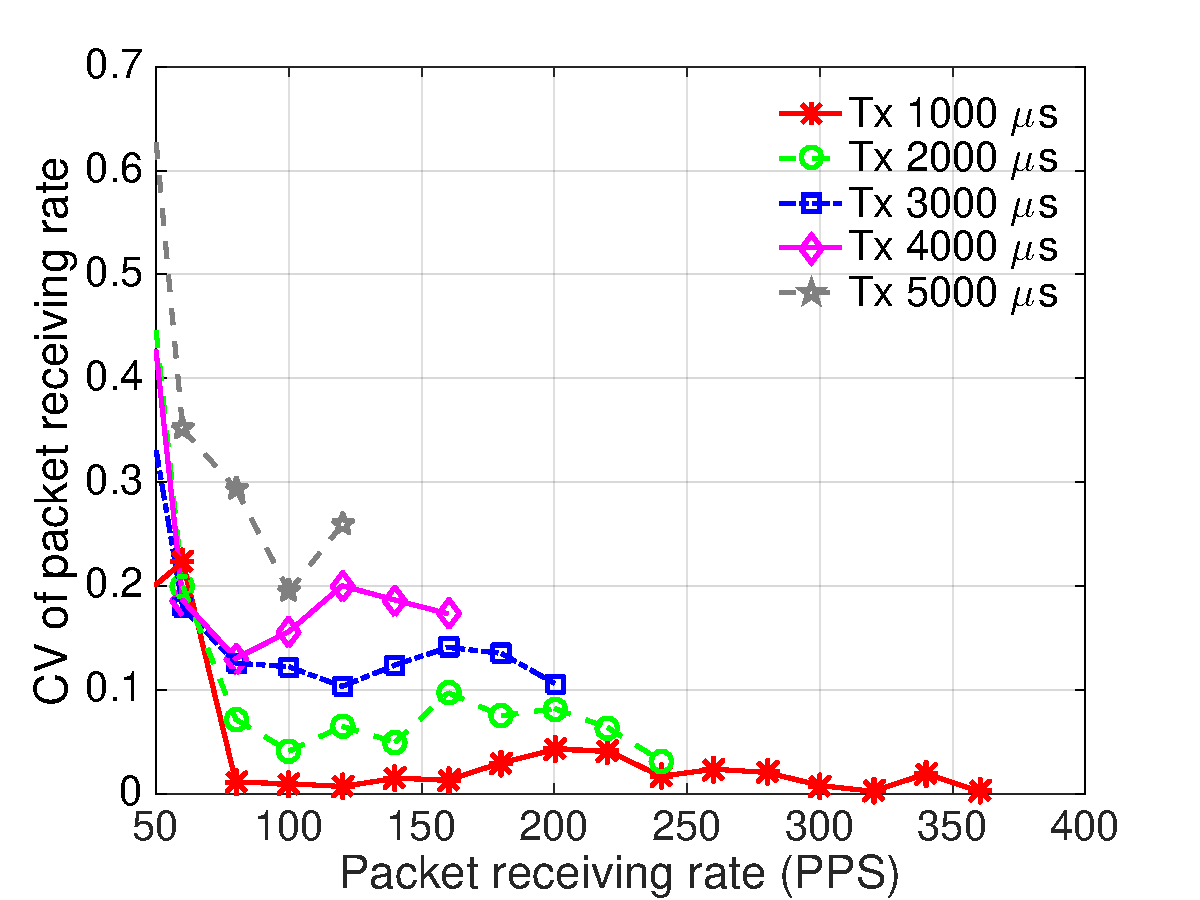
\includegraphics[width=0.45\textwidth]{figures/new_load_avg_result_Prate_tx_all}} 
    \subfloat[Data points with packet receiving rate larger than 60 and \gls{pdr} larger than 0.8 \label{fig:tx-diff-Prate-08}]{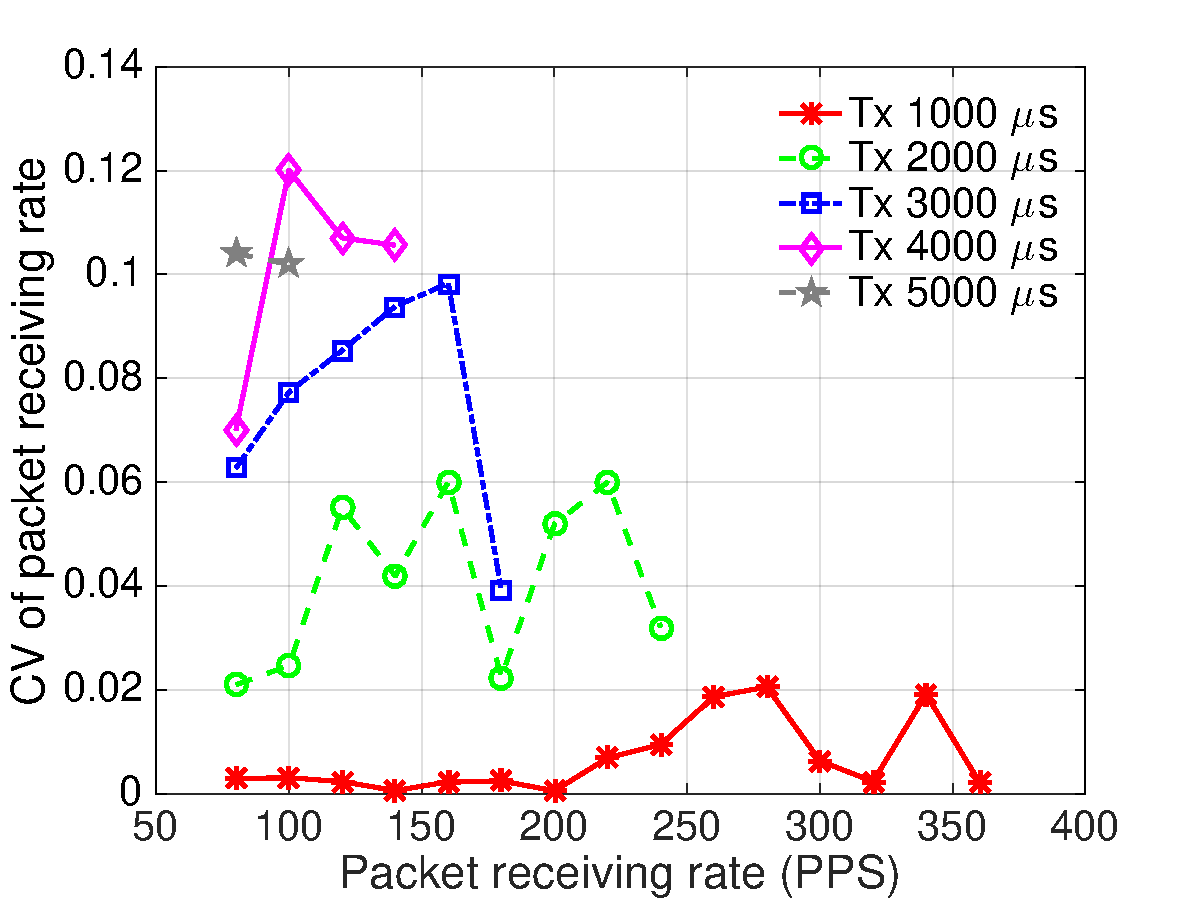
\includegraphics[width=0.45\textwidth]{figures/new_load_avg_result_Prate_tx_all_08_L60}}
  \caption{\gls{cov} of packet receiving rate as a function of packet receiving rate for different average transmission time. 
  %consisting of different coverage and packet size ranges..
  \label{fig:tx-diff-Prate}}
\end{figure*}


\begin{figure*}[t]
    \centering
    \subfloat[All data points  \label{fig:tx-diff-load-all}]{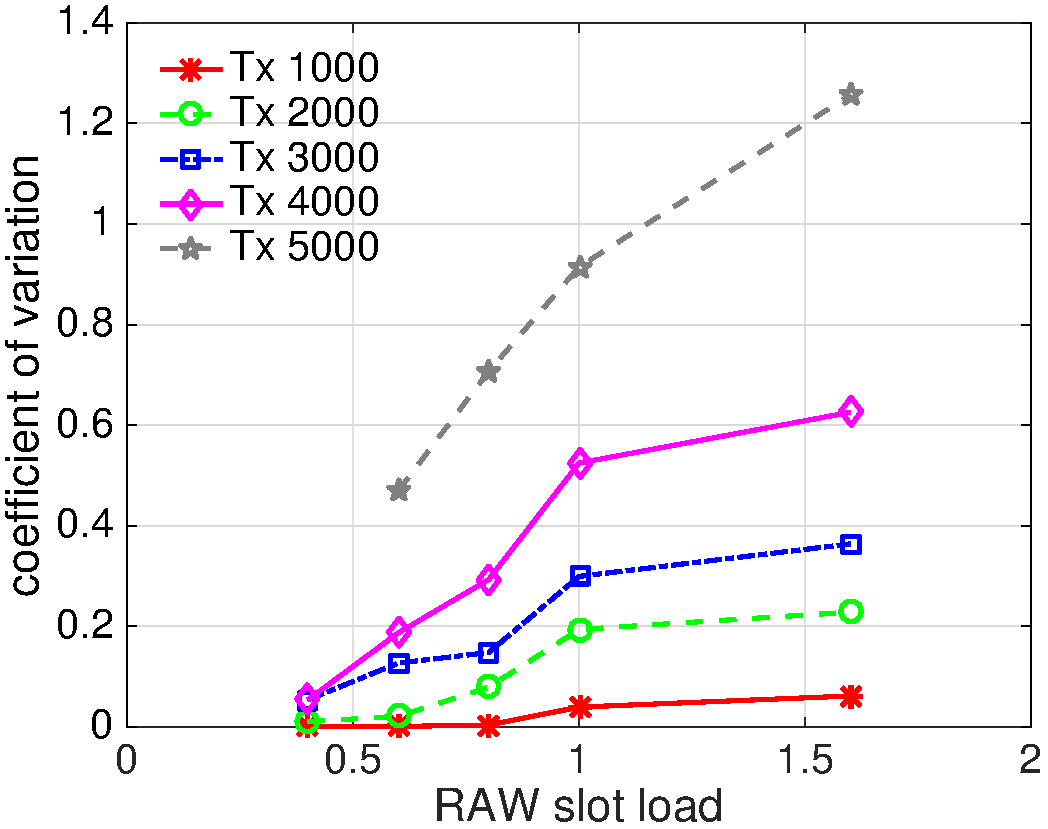
\includegraphics[width=0.45\textwidth]{figures/result_new_load_cov}} 
    \subfloat[Data points with packet receiving rate larger than 60 and \gls{pdr} larger than 0.8 \label{fig:tx-diff-load-08}]{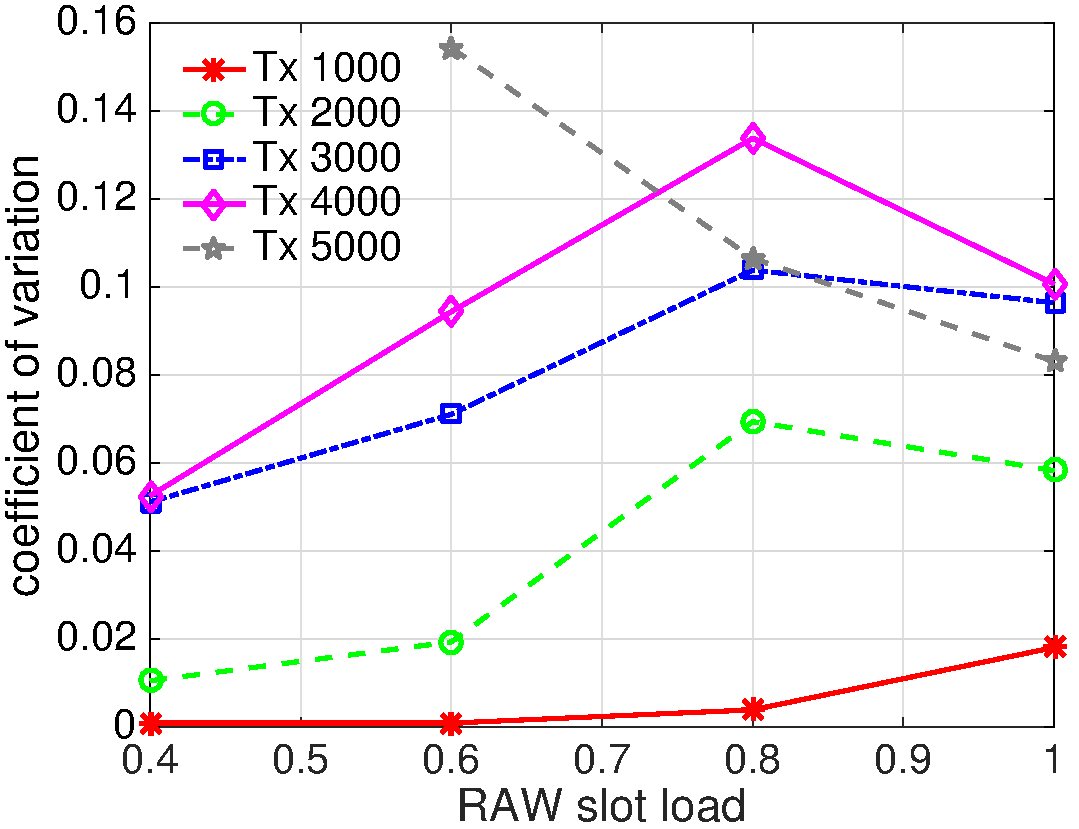
\includegraphics[width=0.45\textwidth]{figures/result_new_load_cov_08}}
  \caption{\gls{cov} as a function of \gls{raw} slot load rate for different average transmission time.
  %consisting of different coverage and packet size ranges..
  \label{fig:tx-diff-load}}
\end{figure*}



%\gls{cov} is a measure of variation or dispersion of a set of data values, it is calculated by dividing the standard deviation of a series of values by the average of the values.


%it is vital that the networks with the same average transmission time have the similar behaviour, i.e., similar packet receiving rate, in order to accurately predict one for the other.



%The CV or RSD is widely used in analytical chemistry to express the precision and repeatability of an assay. 

%As an average transmission time can consist of a variety of packet size range that can affect the throughput, the successfully packet receiving rate  (i.e., number of packet per seconds) is used as the metric of the performance. The throughput can be subsequently calculated together with the packet size range for a specific network scenario.

%In order to proof the viability of using average transmission time as the input parameter representing the network conditions, we compare the performance ( i.e., packet receiving rate) of different coverage and packet size ranges, which all results in the same average transmission time $T_x$. 




The variance is evaluated under different packet receiving rate and \gls{raw} slot load ratios. The \gls{raw} slot load ratio is defined as the ratio between the required transmission time of the 
packets that are allowed to transit in a \gls{raw} group, and duration of the \gls{raw} group. Its definition is as follows:
 \\
\begin{equation}
\mathcal{L}_{r} = \frac {n_r \times TXOP} {d_r \times \mathcal{T}_s}. 
\end{equation}
\begin{equation}
TXOP = T_x + T_{SIFS} +  T_{ACK}
\end{equation}
Where $TXOP$ indicate the time including data packet transmission time $T_x$, a SIFS time (160 $\mu$s) and the ACK transmission time (1000 $\mu$s). $\mathcal{T}_s$ represents the packet sending interval of a station. A large value means a high input traffic load, and vice versa. The network is under overloaded traffic condition when slot load ratio is larger than 1.
%The minimal slot traffic load which can cause performance discrepancy is denoted as $\mathcal{L}_r^max$, in order to apply the model to the extended design space, the slot traffic load needs to be no larger than the $\mathcal{L}_r^max$. For transmission time $1000$ and $5000$ \textit{us}, the  $\mathcal{L}_r^max$ are \textcolor{red}{xx} and \textcolor{red}{xx}, respectively.
In the evaluation, 500 design points for each average transmission times (i.e., 1000, 2000, 3000, 4000 and 5000 $\mu$s) are randomly selected, 
consisting of 5 different \gls{raw} slot load ratio (i.e., 0.4, 0.6, 0.8, 1.0, 1.6). Each data point has four input parameters, i.e., number of station, number of slot, \gls{raw} duration, and average transmission time. The simulation runs 10 times for each data point. During each simulation, the simulator randomly selects a different coverage and packet size range satisfying the required average transmission time. After simulation, the \gls{cov} of each data point's output (i.e., packet receiving rate) is calculated. Subsequently, for each average transmission time, the \gls{cov} is averaged, among the data points with the same packet receiving rate and \gls{raw} slot load ratio respectively. The final results are shown in Figure \ref{fig:tx-diff-Prate} and \ref{fig:tx-diff-load}, each includes the results of both all data points and only the data points with \gls{pdr} larger than 0.8.
%It turns out, the performance variability of the network \textcolor{red}{ (data point) is relevant} to  average transmission time, packet receiving rate, and \gls{raw} slot load ratio.



Figure \ref{fig:tx-diff-Prate-all} shows that, small packet receiving rate (i.e., less than 60) can result in quite high performance discrepancy, with \gls{cov} 1.009 and 2.08 for average transmission time 1000 $\mu$s and 5000 $\mu$s respectively. For the larger packet receiving rate, the \gls{cov} is around 0.25 for average transmission time 4000 $\mu$s and 5000 $\mu$s, the variance is still high. However, when focus on the data points with packet receiving rate larger than 60 and \gls{pdr} larger than 0.8, the \gls{cov} is significantly reduced, as depicted in Figure \ref{fig:tx-diff-Prate-08}. Moreover, the smaller average transmission time results in less variability, while the larger average transmission time leads to more variability. For example, the \gls{cov} is at most 0.02, between 0.02 and 0.07, for average transmission time 1000 and 2000 $\mu$s respectively. While for average transmission time 5000 $\mu$s, the \gls{cov} ranges from 0.10 to 0.16. It should be noted that, the maximum achievable packet receiving rate decreases as the average transmission time increases, since more time is needed for one packet transmission.
%The high performance discrepancy for small packet receiving rate make sense, as a small value more easily leads to a large discrepancy. 
% the smaller average transmission time results in less variability, while the larger average transmission time leads to more variability. Moreover, a small packet receiving rate (i.e., less than 60) results in quite high performance discrepancy, with \gls{cov} 1.009 and 2.08 for average transmission time 1000 $\mu$s and 5000 $\mu$s respectively. For larger packet receiving rates, the performance remains stable, the \gls{cov} is less than 0.03 and around 0.06 for average transmission time 1000 and 2000 us, around 0.12 and 0.15 for average transmission 3000 and 4000 us, and 0.25 for average transmission time 5000 us. The high performance discrepancy for small packet receiving rate make sense, as a small value more easily leads to a large discrepancy. It should be noted that, the maximum achievable packet receiving rate decreases as the average transmission time increases, since more time is needed for one packet transmission.
Figure \ref{fig:tx-diff-load-all} again demonstrates that, average transmission time has a significant impact on the performance discrepancy. Furthermore, it reveals that the performance variation increases with larger \gls{raw} slot load. However, except for average transmission time 1000 $\mu$s, the \gls{cov} is quit high (above 0.2) in most cases. By only focusing on the data points with \gls{pdr} larger than 0.8, the \gls{cov} can be significantly reduced, as depicted in Figure \ref{fig:tx-diff-load-08}.
For example, the \gls{cov} is 0.001 and 0.02 for \gls{raw} slot load ratio 0.4 and 1.0 when average transmission time is 1000 $\mu$s. For average transmission time 3000 $\mu$s, The \gls{cov} ranges from 0.05 to 0.1,  from 0.1 to 0.16, for  average transmission time 3000 and 5000  $\mu$s, respectively. 



 %The higher \gls{raw} slot load ratio means more fierce condition, 

%Figure \ref{fig:tx-diff-load}, only the data points whose packet receiving rate is more than 60 are depicted. The result again demonstrates that, average transmission time has a significant impact on the performance discrepancy. Furthermore, it reveals that the performance variation increases with larger \gls{raw} slot load. 
% For example, for average transmission time 1000 $\mu$s, the \gls{cov} is 0.009 and 0.05 for \gls{raw} slot load ratio 0.4 and 1.6 when average transmission time is 1000 $\mu$s. 
% %For average transmission time 3000 us, the \gls{cov} is 0.05 and 0.15 for \gls{raw} slot ratio 0.4 and 0.8, increase to 0.18 for overloaded traffic (i.e, \gls{raw} slot ratio 1.6).  
% While for average transmission time 5000 $\mu$s, the \gls{cov} is relative large, ranging from 0.18 to 0.41 when \gls{raw} slot ratio increases from 0.6 to 1.6. \todo{reason}
% The higher \gls{raw} slot load ratio means more fierce condition, 



 
Since the trained \gls{raw} model is mainly used for performance optimization, mainly the data points with large packet receiving rate are and high \gls{pdr} are our focus, 
based on the results shown in Figure \ref{fig:tx-diff-Prate} and \ref{fig:tx-diff-load}, we can conclude that  average transmission time is able to represent the conditions of network. Therefore, in this paper, we use the average transmission time as a input parameter for the training.
 
The fact that the performance variance are affected by factors, including packet receiving rate, \gls{raw} slot load ratio, \gls{pdr} and average transmission time, can be explained as follows. 
%  The large \gls{cov} exists for small packet receiving rate is due to the fact that a small values is more easily leads to a large variance. As the networks (i.e., data points) have different input parameters, even the networks sharing the same input parameters may have different coverage and packet size ranges, there are different saturated levels for these networks. With larger \gls{raw} slot ratio, the channel contention is more fierce, therefore, the performance of different networks are more discrepancy. Data points with higher \gls{pdr} implies that, they have proper \gls{raw} configurations that mitigate the channel contention, leading to higher saturated levels. Therefore, less performance discrepancy among different networks is obtained. 
 \begin{itemize}
 \item \textbf{Packet receiving rate} \\
 The large \gls{cov} exists for small packet receiving rate is due to the fact that a small values is more easily leads to a large variance.
 \item  \textbf{\gls{raw} slot load ratio} \\
 As the networks (i.e., data points) have different input parameters, even the networks sharing exactly the same input parameters may have different coverage and packet size ranges, there are different saturated levels for these networks. With larger \gls{raw} slot load ratio, the channel contention is more fierce and more networks reach their saturated levels, therefore, the performance of different networks has more discrepancy.
 \item \textbf{\gls{pdr}} \\
 Higher \gls{pdr} implies that, these data points have proper \gls{raw} configurations that mitigate the channel contention, leading to higher saturated levels. Therefore, less performance discrepancy among different networks is obtained.
 \item \textbf{Average transmission time} \\
 For each network with average transmission time $T_x$, Figure \ref{fig:tx-std-dist} depicts its standard deviation of packet transmission time across all stations. It shows, for networks with a same and lager average transmission time, there is a higher chance that these networks have different packet transmission time distribution. Such difference can result in performance discrepancy when packet collision happens, as the airtime wasted by collision and required by re-transmission depends on the transmission time of collided packets.
  \end{itemize}


%  average transmission time can represent the conditions of network, which has small average transmission time, large packet receiving rate and non-overloaded traffic. In this paper, we use the average transmission time as a input parameter for the training, due to the following three reasons. First of all, the trained \gls{raw} model is mainly used for performance optimization, mainly the data points with large packet receiving rate are interesting. Second, overload traffic is not common in realistic scenarios, we only need to focus on the non-overloaded traffic scenarios. Last but not least, as mentioned in section \ref{subsec:network_para_design}, compare to parameters {${d^-}$, ${d^+}$, ${ps^-}$, ${ps+}$}, average transmission time $\hat{p_p}$ lead to an input design space with only xx data points. Therefore, there is a trade-off between the accuracy and training speed. \textcolor{red}{Tx 5000 us results in high performance discrepancy, should we mentioned the model is not suitable for Tx 5000?}. During the training, network scenarios with the same average transmission time use a fixed coverage range and packet size range. 

% explanation
%The performance discrepancy of an average transmission time for different coverage and packet size ranges is mainly caused by the propagation loss, capture effect. As the location and packet size distribution among stations is different. As small average transmission time, for example transmission time $1000$ us, has relative short distance  and packet size, leading to small variance on the packet rate. While for large transmission time, stations have longer distance to the \gls{ap} and larger packet size, therefore, the packet rate has larger variance. \todo{update the explanation.}


% To build the surrogate model, the input parameter space needs to be defined. It consists of the minimum and maximum value of each parameter, as well as a step size. The minimum and maximum can be determined based on expert knowledge of \gls{raw} performance, as well as legal values defined by the IEEE~802.11ah standard. The range of the number of stations $n_r$ in a \gls{raw} group should span from low to high traffic conditions, so the trained model gives accurate results independent of the density. From our previous studies on \gls{raw} performance~\cite{wowmom2018}, for MCS with bandwidth 1 MHz and packet size less than 512 bytes, a minimum value of $60$ and maximum value of $400$ stations per group were deemed to cover all possible traffic conditions. The number of slots $s_r$ is bound between $1$ and $64$, as per the IEEE standard. However, a very high number of slots leaves not enough time within a slot to successfully transmit a packet. As such, we limit $s_r$ between 1 and 50. The RAW group duration should be large enough to allow at least 1 packet is successfully sent in each \gls{raw} slot, and at most equal to the duration of the beacon intervals. As such, by taking the \gls{raw} slot number into account, $d_r$ is varied between $40960$~$\mu$s and $204800$~$\mu$s.


% 
%Several aspects are involved:
%1, the same average transmission time can results in different output.
%2, the same network (coverage and packet size range) can have quite different outputs for different randomization seeds.
%3, load ratio also play an ratio, the performance difference among networks with same average transmission time increases when load ratio increase.


% The actual step size of $n_r$, $s_r$ and $\hat{t}_p$ is $1$, as they are integer variables. The parameter $d_r$ has a step size of $120$~$\mu$s, as defined in the 802.11ah standard. This results in a total input space of \textcolor{red}{$2.3 \times 10^7$} possible data points. This is too high to properly train the model in a feasible amount of time. To alleviate this, we experimentally determined a good step size for each of the parameters, leveraging the trade-off between accuracy and training speed. For $n_r$ and $s_r$ a step size of 5 was selected, 250 is choose as the step size of  $\hat{t}_p$. It was found that the \gls{raw} duration $d_r$ has a high sensitivity. As such, a small value of $5120$~$\mu$s was chosen as its step size. This results in a significantly reduced input space of \textcolor{red}{$25047$} data points. Table~\ref{tab:sumo parameters} summarizes the selected input parameter space. Note that a slot count $s_r$ equal to $0$ is not legal, and $s_r$ therefore takes on values from the set $\left\{1, 5, 10, ..., 50\right\}$. 


%Results for data points outside the reduced input parameter space are obtained via linear interpolation of the two nearest data points included in the model.




% \begin{figure}
%   \centering
%   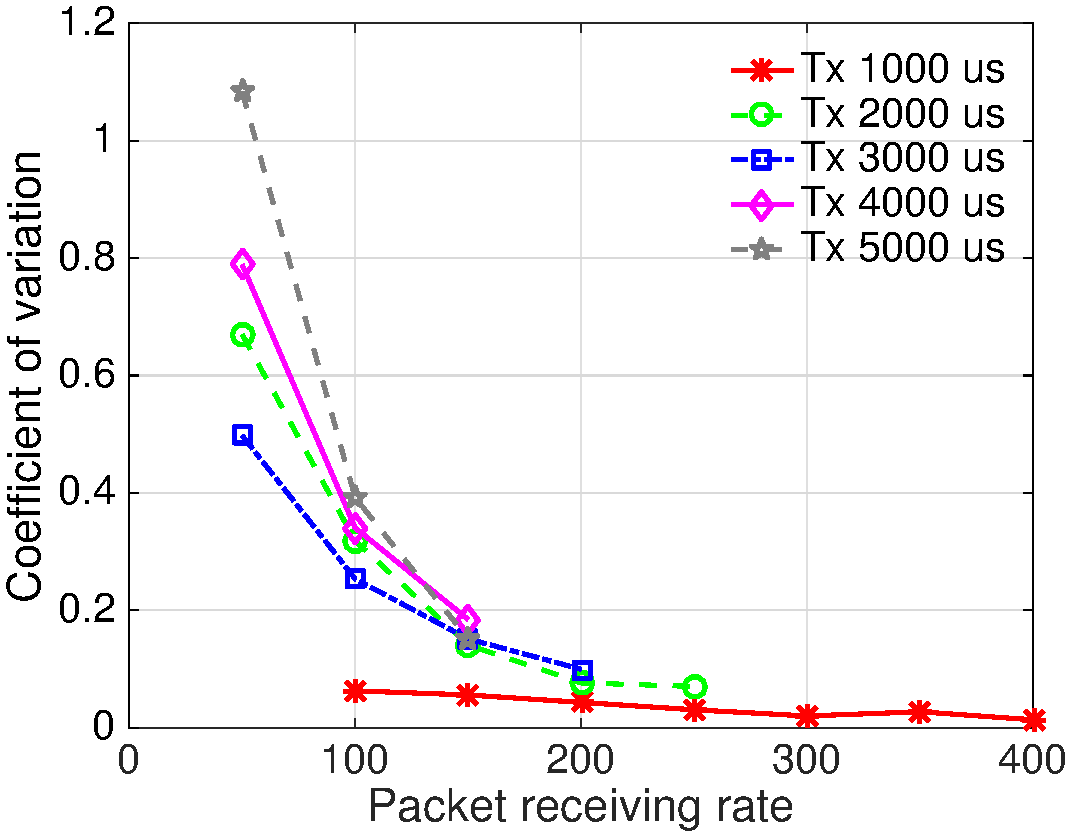
\includegraphics[width=0.75\columnwidth]{figures/avg_result_Prate_tx_ratio3_20}
%   \caption{\textcolor{red}{To be updated}. \label{fig:tx-diff}}
% \end{figure}


% \begin{figure}[t]
%   \centering
%   % 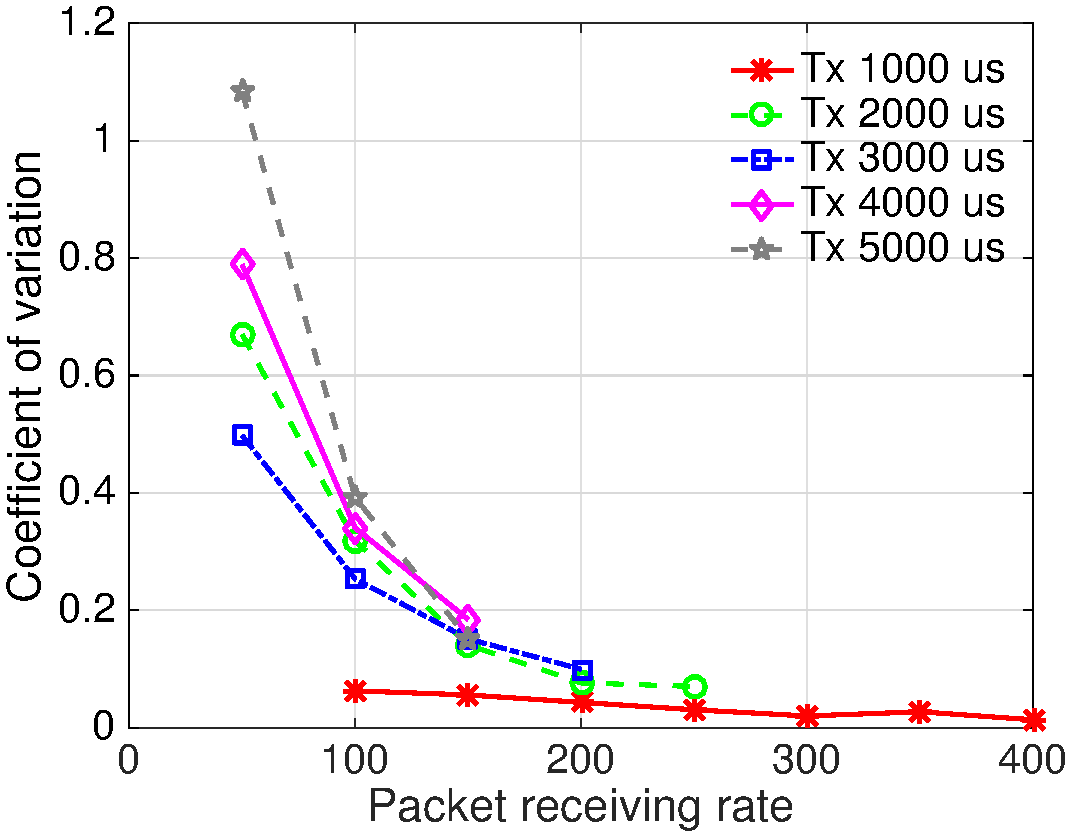
\includegraphics[width=0.75\columnwidth]{figures/avg_result_Prate_tx_ratio3_20.pdf}
% %      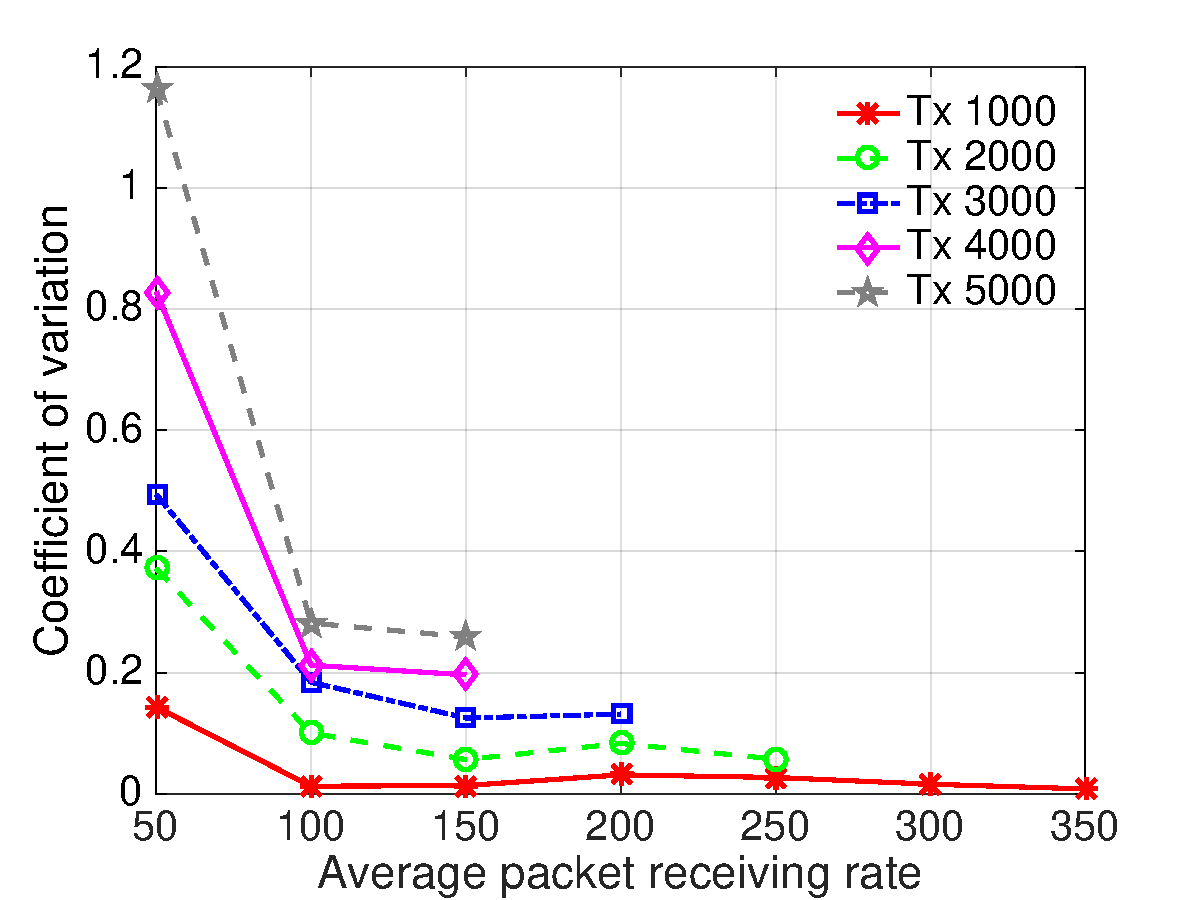
\includegraphics[width=0.75\columnwidth]{figures/avg_result_Prate_tx.pdf}
%   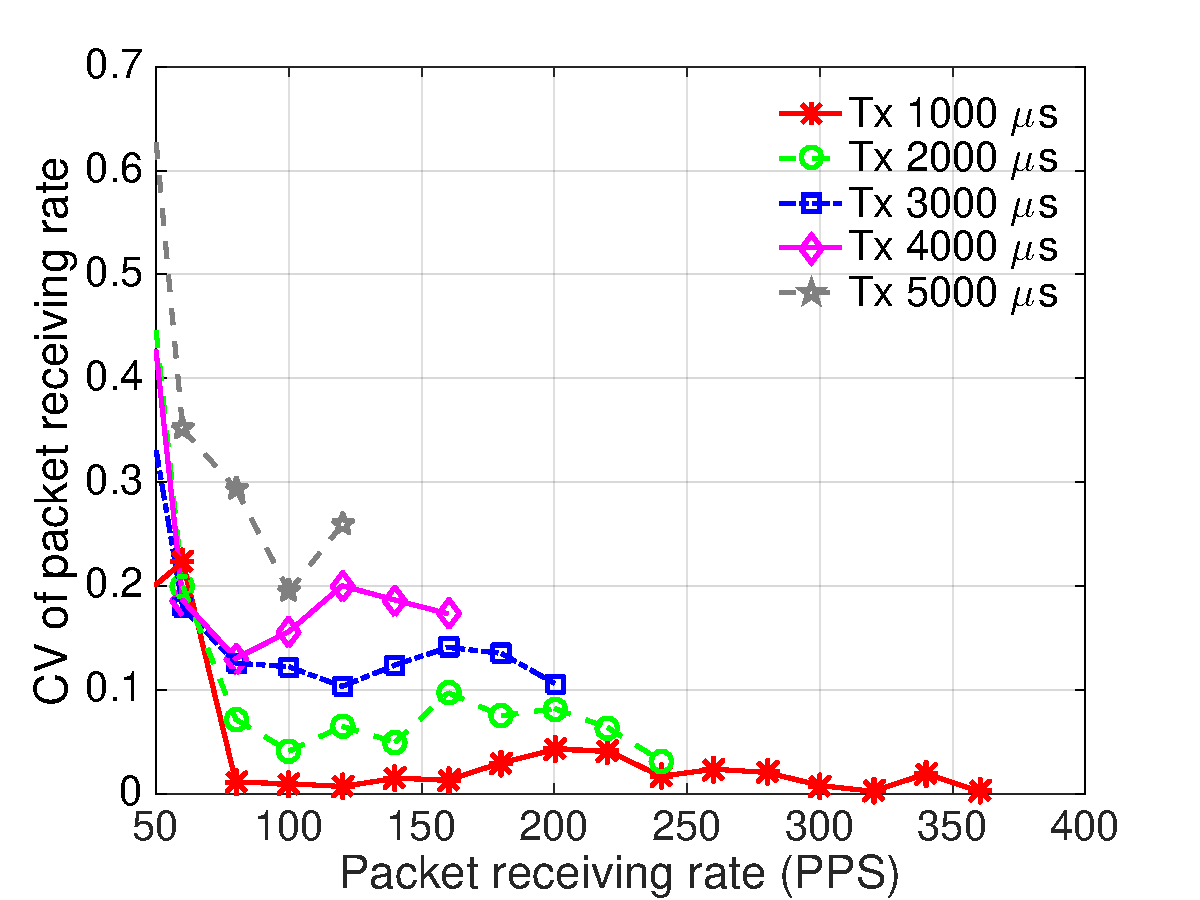
\includegraphics[width=0.75\columnwidth]{figures/new_load_avg_result_Prate_tx_all.pdf}
%     \caption{  \gls{cov} of packet receiving rate as a function of packet receiving rate for each different average transmission time %consisting of different coverage and packet size ranges.
%     \label{fig:tx-diff-Prate}}
% \end{figure}








% \begin{figure}[t]
%   \centering
%   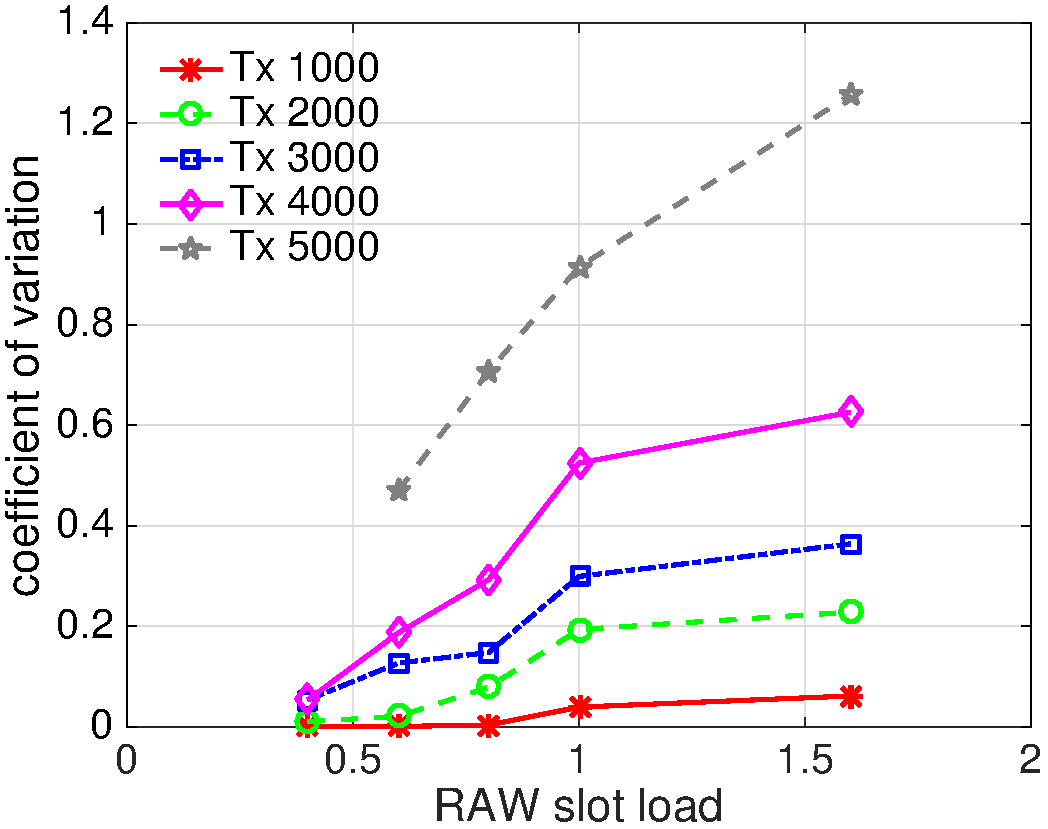
\includegraphics[width=0.75\columnwidth]{figures/result_new_load_cov.pdf}
%     \caption{Coefficient of variation as a function of \gls{raw} slot load rate for each average transmission time consisting of different coverage range and packet size range.
%     \label{fig:tx-diff-load}}
%     % new load ratio 1_8
% \end{figure}



\begin{figure}[t]
  \centering
  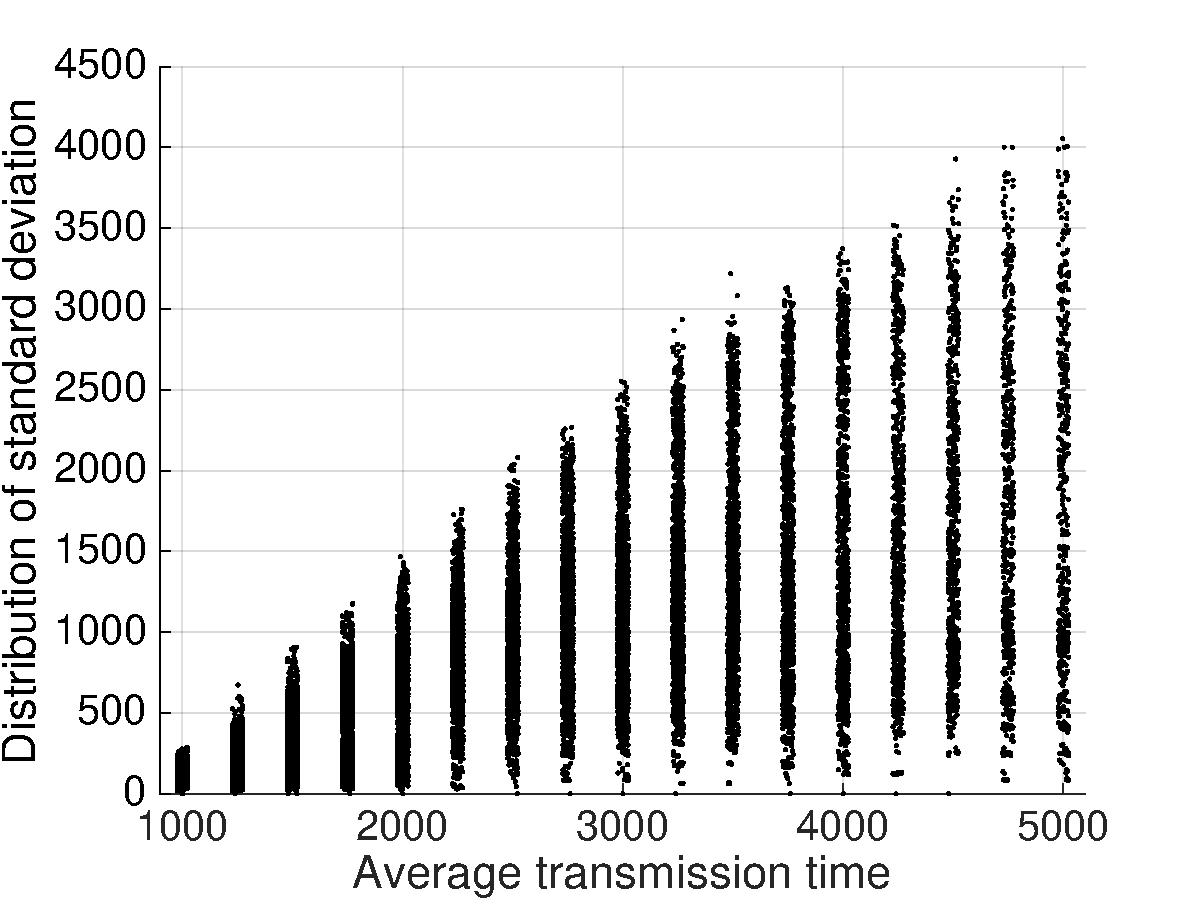
\includegraphics[width=0.85\columnwidth]{figures/std-txtime-distribution}
  \caption{Distribution of standard deviation for different average packet transmission time. \label{fig:tx-std-dist}}
\end{figure}





% \begin{figure}[t]
%     \centering
%     \subfloat[Tx 1000-4000 us  \label{fig:tx-diff-load}]{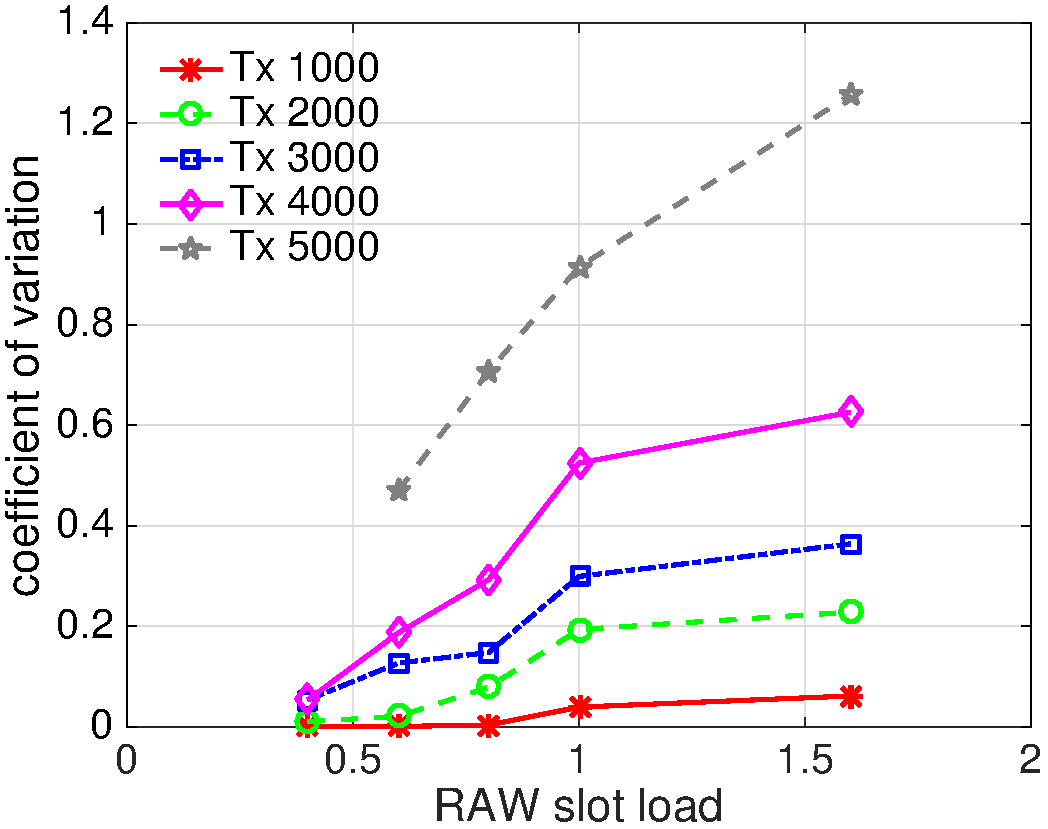
\includegraphics[width=0.8\columnwidth]{figures/result_new_load_cov.pdf}} \\
%     \subfloat[Tx 4000-5000 us  \label{fig:tx-diff-Prate}]{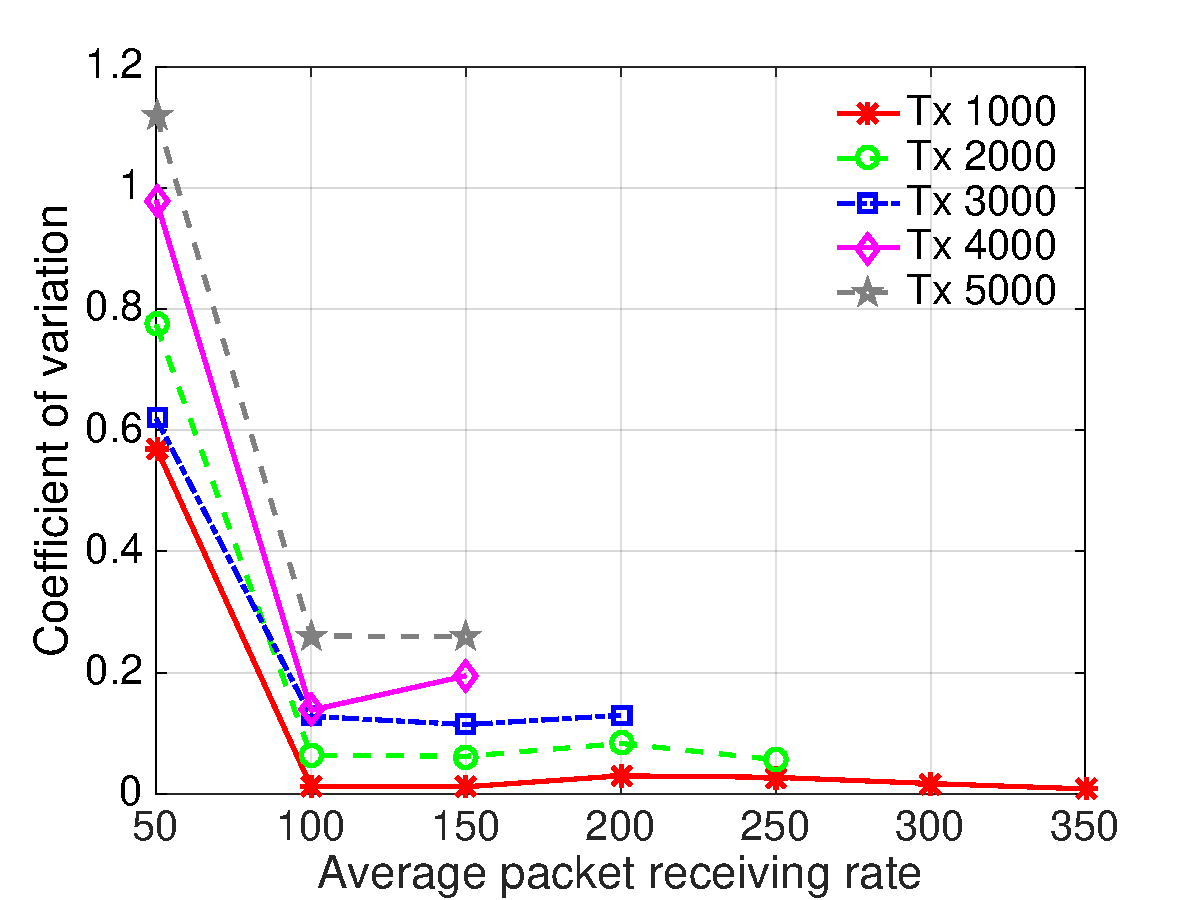
\includegraphics[width=0.8\columnwidth]{figures/new_load_avg_result_Prate_tx.pdf}}
%   \caption{Coefficient of variation as a function of packet receiving rate for each average transmission time consisting of different coverage range and packet size range  \label{fig:tx-diff}}
% \end{figure}



% \begin{figure}
%   \centering
%   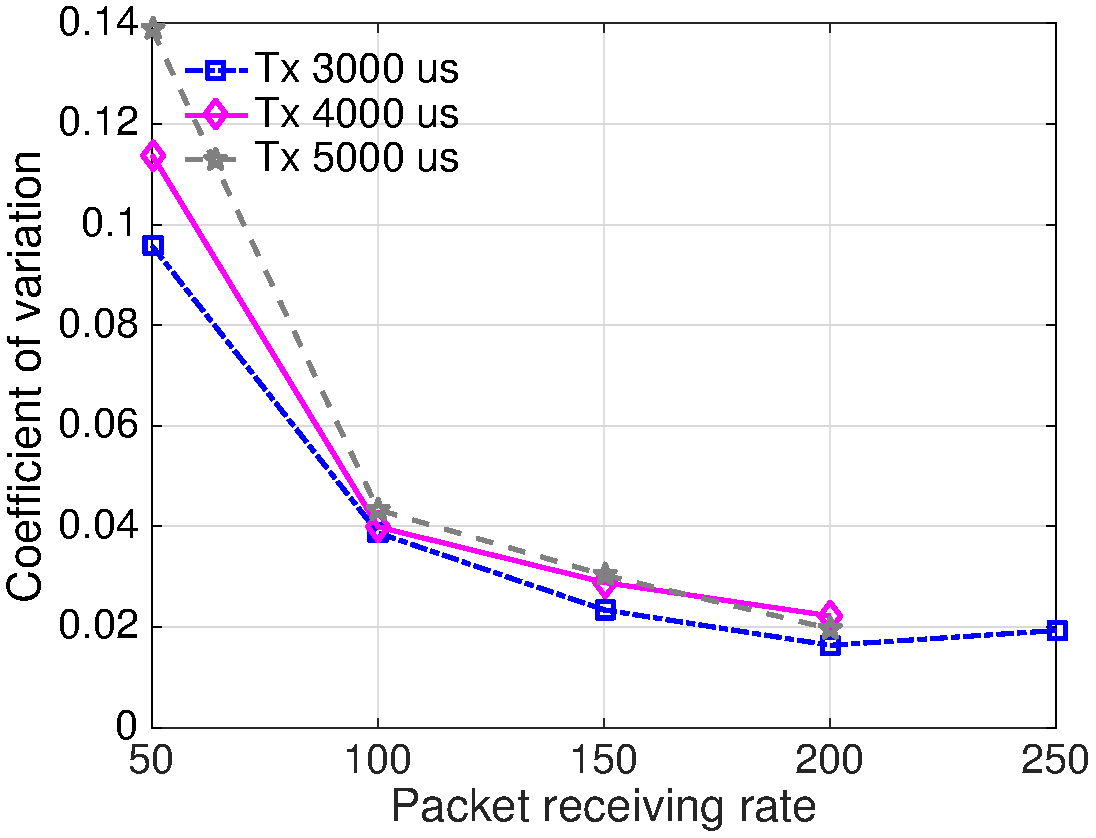
\includegraphics[width=0.75\columnwidth]{figures/avg_result_Prate_tx_ratio3_20_line}
%   \caption{result of different tx time with line. \label{fig:tx-diff-line}}
% \end{figure}




 

% The results in previous section have demonstrated that the created model has quite good accuracy on predicting the output of a given \gls{raw} configuration. In this section, we explore the performance of the model when the average transmission time are generate by  distance and packet size ranges that are not used during the modeling process.

% The variable used by the \gls{raw} modeling, \textit{average transmission time}, is actually represented by two parameters of the 802.11ah network, i.e., distance between stations and \gls{ap}, and packet size of the stations. 



 %\item Training methodology (the evaluation scenario used for training)
\subsection{Training methodology \label{subs:raw_training}}

% Surrogate modeling provides the answer \cite{SUMOtoolbox2010}. 
% A surrogate model is trained at design
% time, using a limited number of input-output sample data
% points obtained through simulation or real-life experiments.
% Surrogate modeling is especially suited for tasks with a large
% input space, as an accurate model can be trained based on
% relatively little input data points. Moreover, evaluating the
% model at runtime is computationally efficient, equivalent to
% a constant-time table lookup. This makes surrogate modeling
% highly suitable for RAW performance modeling, as the input
% space is very large, and efficient runtime model evaluation is
% needed for real-time RAW parameter selection. Additionally,
% by using realistic simulation results, a surrogate model does not suffer from the same restrictive assumptions as existing
% analytical models.

The training of RAW performance surrogate model follows the below steps, using the same numbering as the arrows in Figure \ref{fig:sumo-ns3}:
%When a new sample data point is generated for which the output is unknown, the controller will initiate an ns-3 simulation to determine the output associated with the input parameter values of the data point. 

\begin{enumerate}

\item \label{sm_tr_1} Based on the defined design space (cf. Table~\ref{tab:sumo parameters}), the initial design points are carefully selected to efficiently characterize the system. Each data point has four input parameters, i.e., number of stations, number of slots, \gls{raw} duration, and average transmission time.

%The latin hypercube design (LHD) method is used here to select the design points. It is the most commonly used approach for intial design points selection, selecting sample points evenly along the configuration space while ensuring proportional representation of design variables.

\item \label{sm_tr_2} The ns-3 simulator executes experiments with parameters from each initial data point and the general parameters of 802.11ah (cf. Table~\ref{tab:ns3 parameters}). The evaluation criterion (e.g., packet receiving rate) of the experiments are considered as the output of each data point. 

\item \label{sm_tr_3} After the experiments with all the initial data points, an initial surrogate model is created.

%and calculates the cross validation score. If the score is below the threshold, the experiment stops executing. Otherwise, it continues with the next step.

\item \label{sm_tr_4} The sampling strategy is applied to select a few number of next data points to improve the model accuracy.

\item \label{sm_tr_5} The experiments are executed for the newly selected data points, the evaluation criterion of the experiments is considered as the output of the new data points. 

\item \label{sm_tr_6} The surrogate model is updated with the newly selected data points.

\item \label{sm_tr_7}  This process stops once the stop conditions are met, otherwise it continues with step \ref{sm_tr_4}.
\end{enumerate}


Each experiment in ns-3 runs for 60 seconds of simulated time. As \gls{raw} is configured in each beacon interval of 204.8~ms, the results of every simulated configuration are averaged over 290 beacon intervals, ensuring the generality of the trained model. 
%The SUMO toolbox is configured to use 
A proper method is applied in each step in order to create an accurate surrogate model with a limited number of data points. 


\begin{itemize}
\item \textbf{Initial design points selection}  \\
 We use the latin hypercube design (LHD) ~\cite{FAViana2013} approach to select the initial data points, which has the best performance in general and is  most commonly used. It selects sample points evenly along the configuration space while ensuring proportional representation of design variables. Furthermore, the initial sample size depends on the problem type, 200 initial data points was found a good choice for our problem.
 
\item \textbf{The (initial) surrogate model creation}  \\
There are a variety of supervised machine learning and regression methods can be used for surrogate model creation, such as Kriging \cite{forrester2008engineering}, polynomial response surfaces, radial basis functions, support vector machines (SVMs),  space mapping, or artificial neural networks (ANNs). Among these methods, Kriging model is 
very popular in the modeling of  complex systems, including complex wireless network \cite{SUMOWirelessConferencing,wowmom2018, LTEoptimization}.The Kriging model is formed as:
\begin{equation}
\hat{f} (X) = \sum_{i=1}^{V} {a_i}{k(x, x_i)}
\end{equation}
Where $V$ is the amount of basis vectors, $x$ represent the input data vector and $k(x, x_i)$ is the kernel function. There are several kernel (covariance) functions used in Kriging, such as Squared Exponential Kernel, Exponential Kernel, Matern 3/2, Matern 5/2, Rational Quadratic Kernel. Among them, the Matern types of kernel functions are  widely used, and we use the Matern kernel function with %$v=3/2$ and 
$5/2$ to create the model. 

\item \textbf{Sampling strategies} \\
A novel sampling strategy called FLOLA-Voronoi \cite{vanderherten2015} is used to select the next design points to improve the model accuracy.  The FLOLA approach is used for exploiting the non-linear regions, while the Voronoi approach explores the sparsely sampled regions, the scores from  the FLOLA and Voronoi are combined to decide the next sample point. In our experiments, 10 new data points are picked in each interation.

% The initial design points explores the configuration space of the system by applying the appropriate design points selection approaches. However, further exploration is needed since the number initial design points is limited, moreover, the initial model may not exploit interesting regions of the system(i.e., non-linear regions).  Therefore, during the sequential design process, at each iteration, the (Root Relative Squared Error (RRSE)  of the currently created surrogate is checked and new sample points is selected if the model accuracy is not satisfactory. 
 


%  As the non-linear regions are difficult to model compared to linear regions, more sample points are required in the modeling process. Therefore, the FLOLA approach uses the local linear approximations to estimate the linearity of the region, with the aim of further exploring these regions. For the Voronoi part, a Voronoi tessellation diagram is drawn from tested points and  the area of each Voronoi cell is calculated. A smaller area indicates the presence of nearby explored data points, representing a tightly explored region. A wider area indicates the absence of nearby points, or a sparsely explored region.  Finally, the scores from the the FLOLA and Voronoi are combined to decide the next sample point.

\item \textbf{Stopping Criteria} \\
%A stop criteria is needed to terminate the modeling process when the intermediary model is accurate enough.
The 10-fold cross-validation with a \gls{rrse} measure is used to evaluate the model accuracy. The modeling process stops once the cross validation score remains stable (3 digits of precision) for 10 successive iterations, i.e., 100 sample data points. Moreover, the stopping criteria are upper limited to a maximum number (i.e., 10000) of iterations and it will stop execution once the iteration number reaches the limit.
% The training stops once the cross
% validation score lower than or equal to 0:10 (2 digits of
% precision) occurs 10 times in succession, or the number of
% training data points exceeds 2500.


% During the modeling process, the accuracy of model is verified by using cross validation method. At each iteration, the previously obtained samples are divided into training and testing sets, and the predicted response of the model built from the training set is compared against the testing set. The modeling process stops once the cross validation score is below a certain level for a certain number of consecutive iterations. Moreover, the stopping criteria are upper limited to a maximum number of iterations and it will stop execution once the iteration number reaches a specified limit.

\end{itemize}






% To obtain a better initial model, the number of initial sample
% points should be large, however, this increase the training time,
% therefore, a trade-off in terms of the initial design points is
% normally made.





%\end{itemize}

\section{Performance Evaluation and Discussion \label{sec:evaluation}}

This section presents the evaluation results on the \gls{raw} performance predication accuracy of our surrogate model. First, the  convergence of the training process is evaluated. Subsequently, the accuracy of the surrogate model for the reduced design space and the full design space are evaluated respectively. Finally, the optimal \gls{raw} configurations are discussed. As mentioned in Section \ref{subsec:para_design}, there are a number of coverage and packet size ranges that can lead to the same average transmission time. For the reduced design space, the average transmission time is only represented by distance and packet size range used during the training process. While in the full design space, there is no such limitation.

All evaluations are performed using our previously developed
IEEE 802.11ah ns-3 module \cite{WNS32016}, and we consider the same IEEE~802.11ah scenario as described in Section \ref{subsec:80211ah_raw}. The same default PHY and MAC layer parameters are used as shown in Table \ref{tab:ns3 parameters}.

%\subsection{Exhaustive Search Model}
%[Probably too hard to run all these experiments]

\subsection{Training convergence}
%Cross validation score evolution, stopping criterion, ...
\begin{figure}[t]
  \centering
  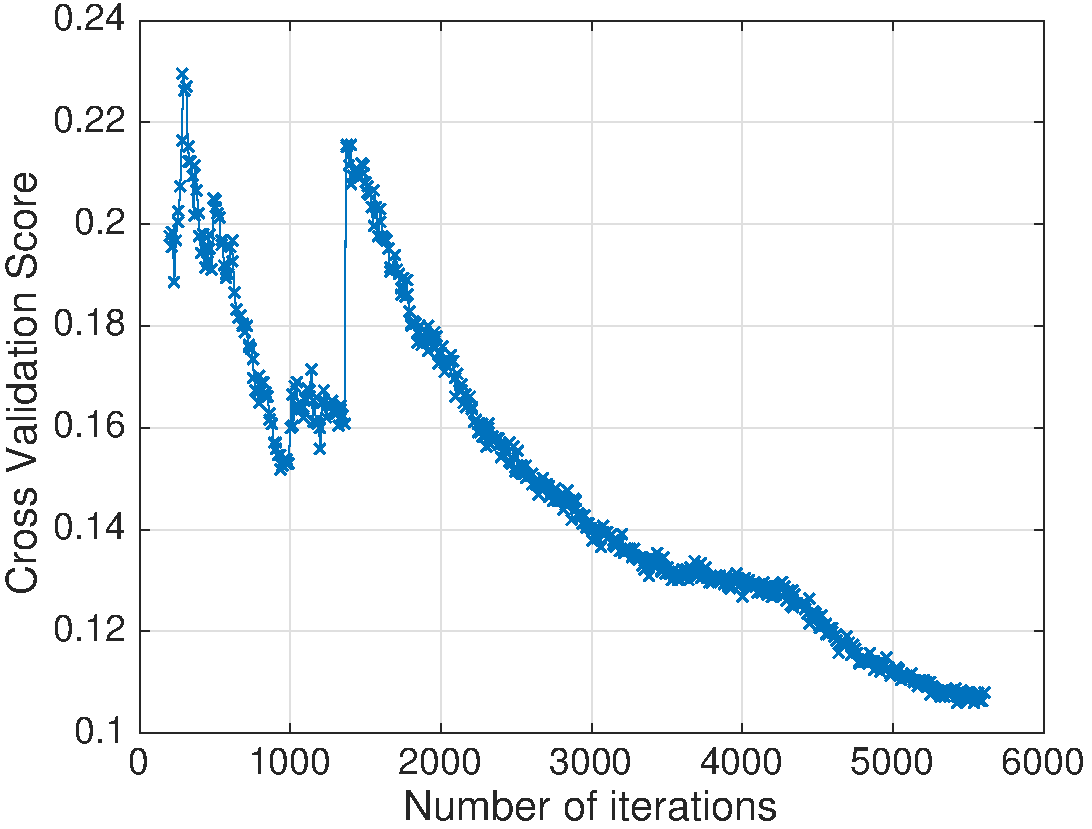
\includegraphics[width=0.75\columnwidth]{figures/throughput-cv}
  \caption{Cross validation score of the surrogate model as a function of the number of training samples. \label{fig:sumo-iteraton}}
\end{figure}

In this section we evaluate the training convergence of
the surrogate model. The cross validation score is widely used to measure the accuracy of the resulting model, a low score signifies the high accuracy of the model, and vice versa. Figure~\ref{fig:sumo-iteraton} demonstrates the 10-fold cross validation score of the model as a function of the number of training samples used, each iteration uses 10 extra samples for training.  %\textcolor{red}{explains the cross validation either in this section or modeling section}.
It clearly shows that at first, SUMO is trying to learn the behavior of the networks with cross validation score going up and down, while from 1360 samples onward, the cross validation score continually decreases until 5520 samples used for training, reaches 0.107. Then the cross validation score remains almost constant, signifying that the training process has converged.  Training of the model stopped after 5610 samples as it satisfied the stop conditions, i.e., 10 consecutive cross-validation scores lower than or equal to $0.107$ (3 digits of precision). This comes down to about 1.3\% of the parameter space (i.e., 425799) defined in table \ref{tab:sumo parameters}, from which samples were drawn during training. It is about only $1.6 \times 10^{-9}\%$ of all data points in the full design space.

% and xx(5600/??) of all data points in the design space (i.e., xx), in which the step size is \textcolor{red}{1} and the results for data points outside the reduced parameter space are obtained via interpolation by the Kriging  model.


%This comes down to about xx(5600/??) of all data points in the input space (i.e., xx), and about xx(5600/425799?) of the reduced data space (i.e., xx) from which samples were drawn during training.



\subsection{Reduced design space experiments}
% \begin{figure*}[t]
%     \centering
%     \subfloat[all \label{fig:throughput-alpha-0}]{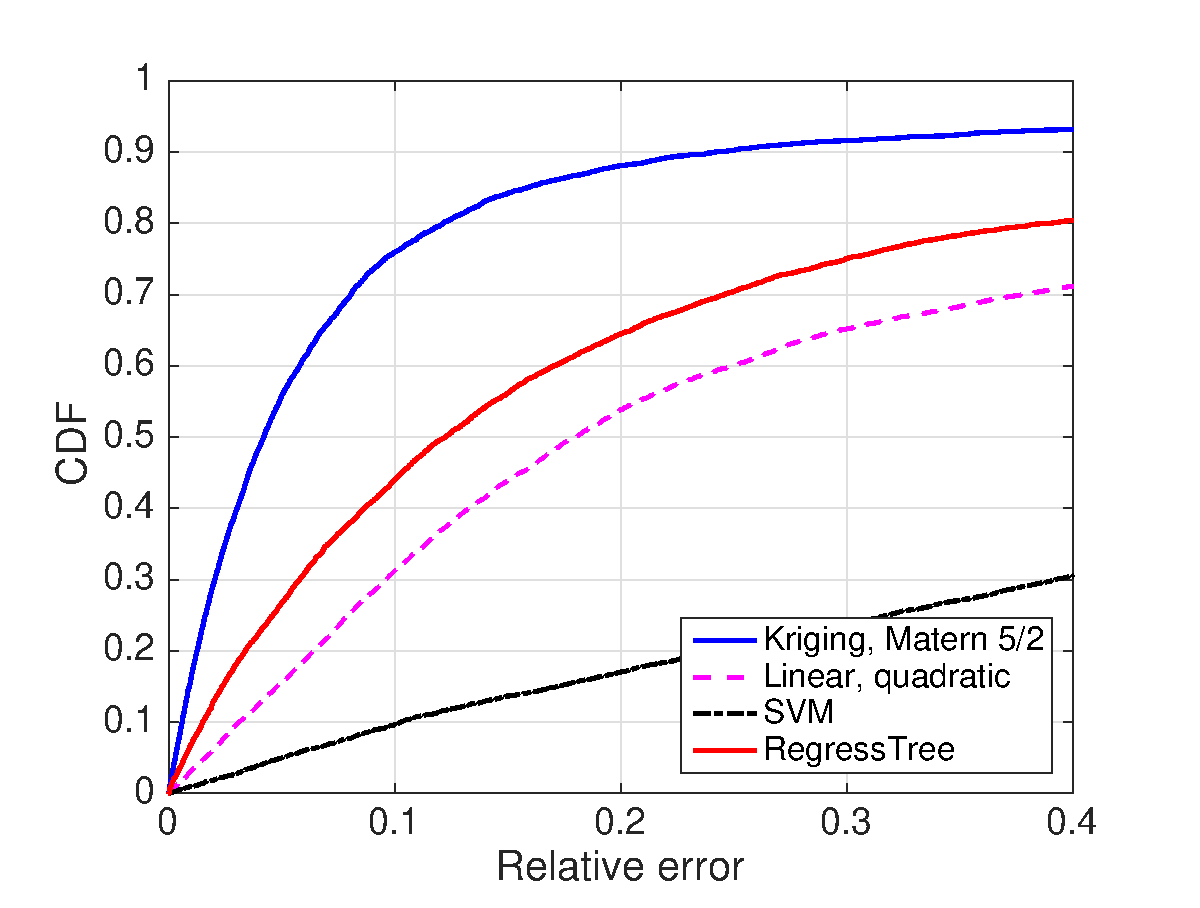
\includegraphics[width=0.30\textwidth]{figures/all}}
%     \subfloat[1\_50 \label{fig:delay-alpha-0}]{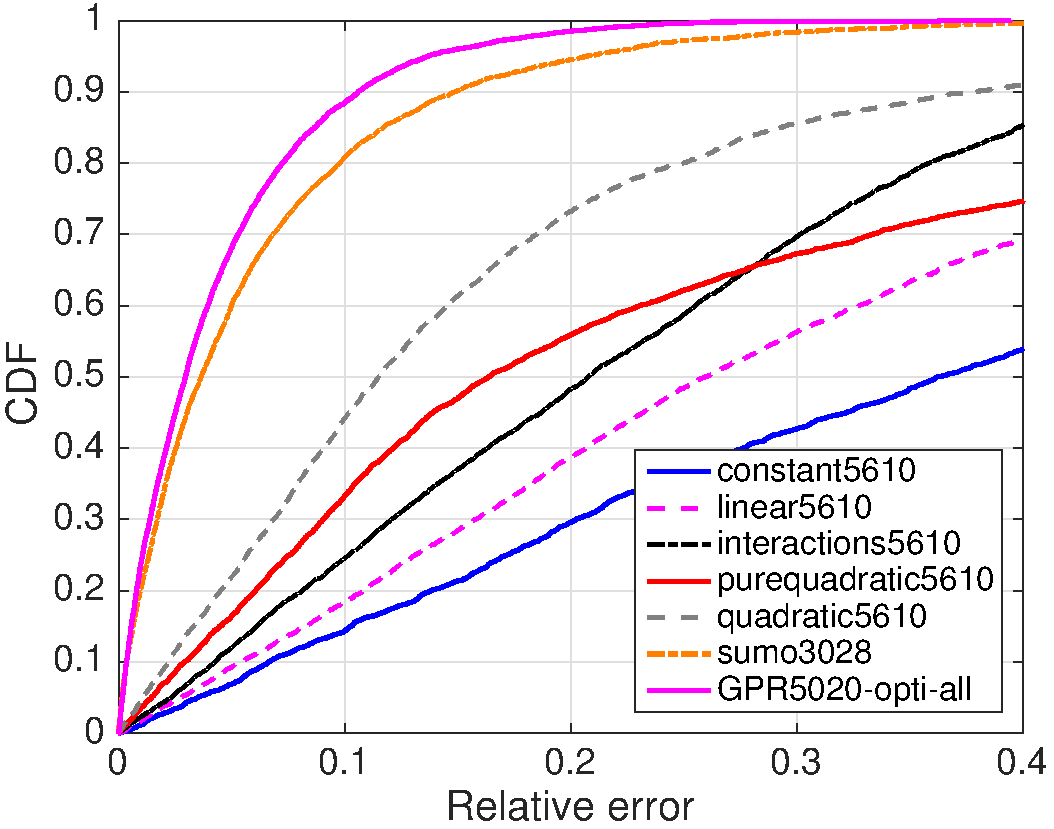
\includegraphics[width=0.30\textwidth]{figures/1_50}}
%     \subfloat[1\_10 \label{fig:delay-alpha-0}]{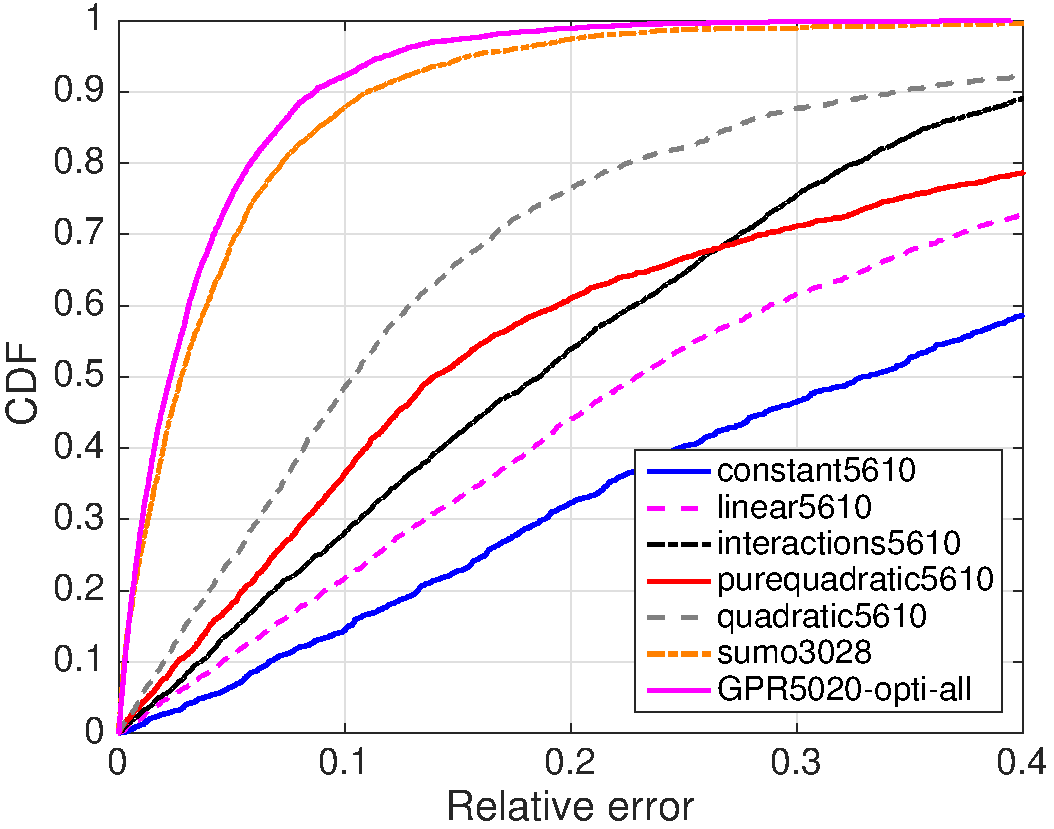
\includegraphics[width=0.30\textwidth]{figures/1_10}}
%   \caption{Comparison of different regression models. \label{fig:regress-models}}
% \end{figure*}


\begin{figure}[t]
    \centering
{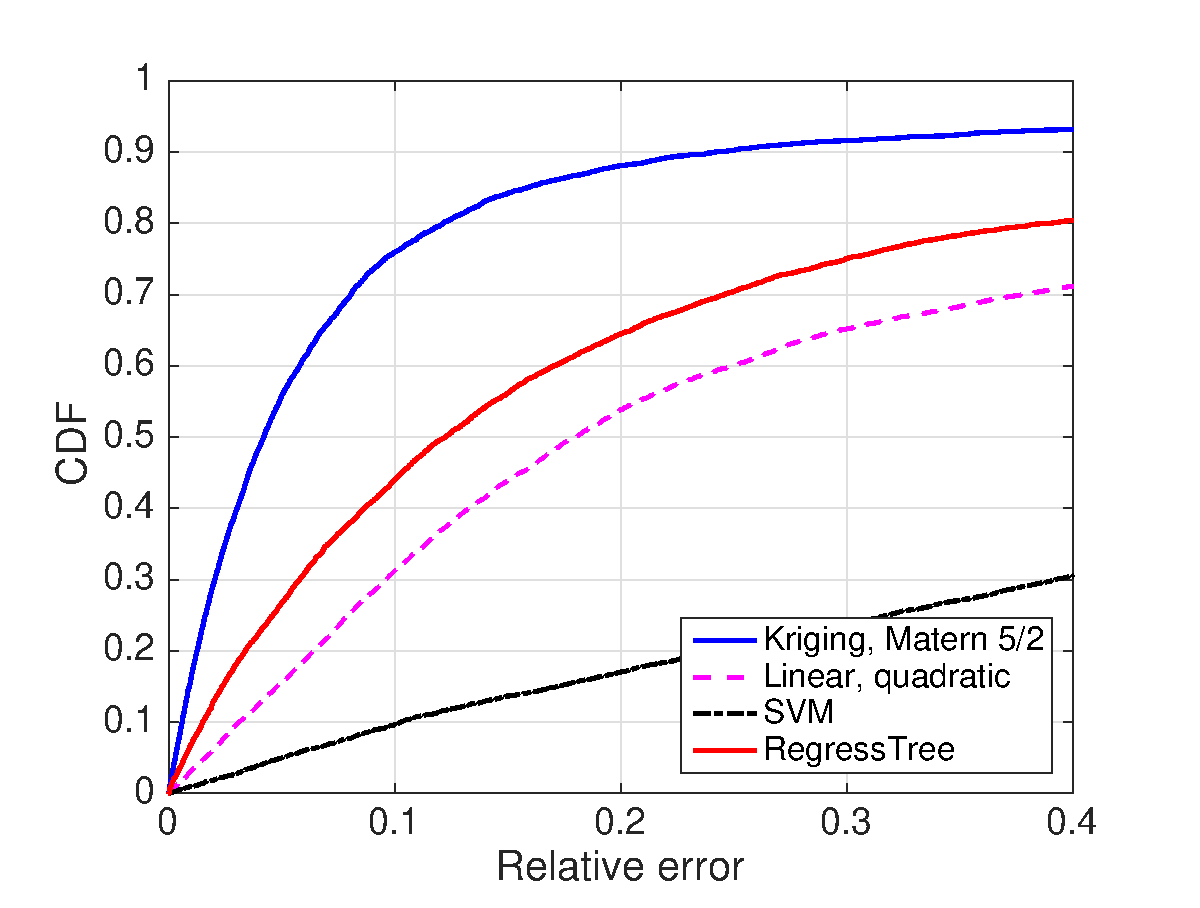
\includegraphics[width=0.8\columnwidth]{figures/all}}
  \caption{Performance comparison between different regression models and simulation results for 6000 random test data
points. \label{fig:regress-models}}
\end{figure}





% \begin{figure}[t]
%     \centering
% {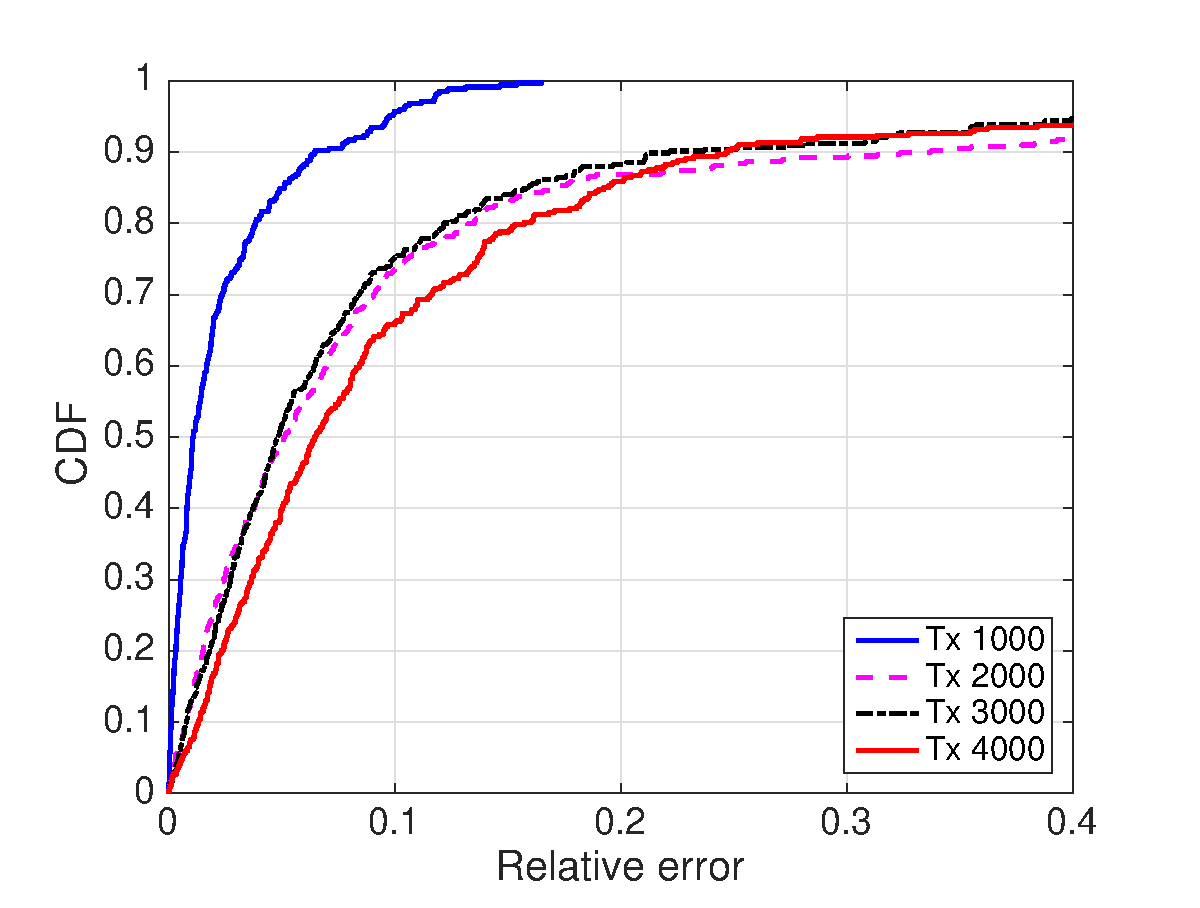
\includegraphics[width=0.8\columnwidth]{figures/cdf_f1000_t4000}}
%   \caption{Comparison of different regression models. \label{fig:regress-models-a}}
% \end{figure}



% \begin{figure*}[t]
%     \centering
%     \subfloat[Relative error $>=$ 0 \label{fig:delay-alpha-0}]{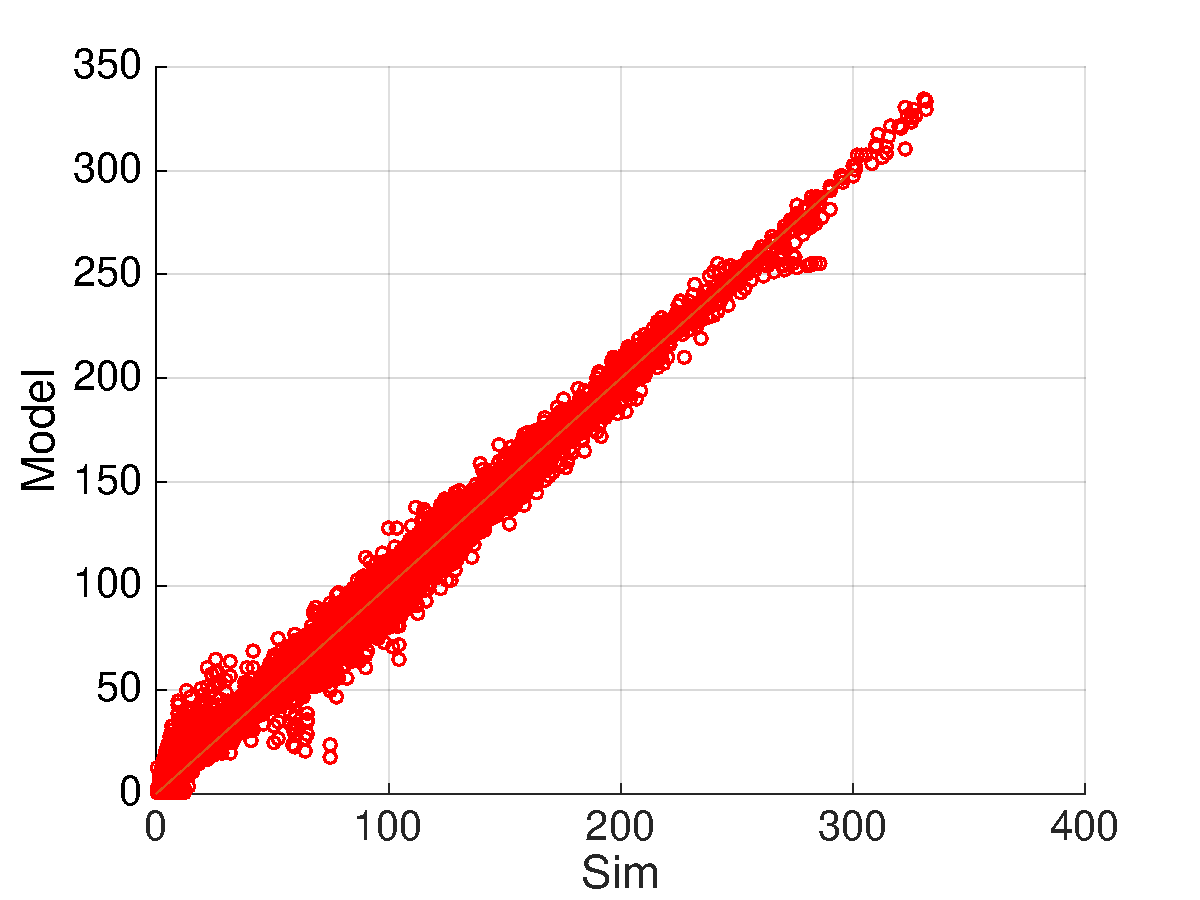
\includegraphics[width=0.33\textwidth]{figures/scatter_results-error-GPR5020-opti-all-sort_L0}}
%     \subfloat[Relative error $>=$ 0.1  \label{fig:delay-alpha-0}]{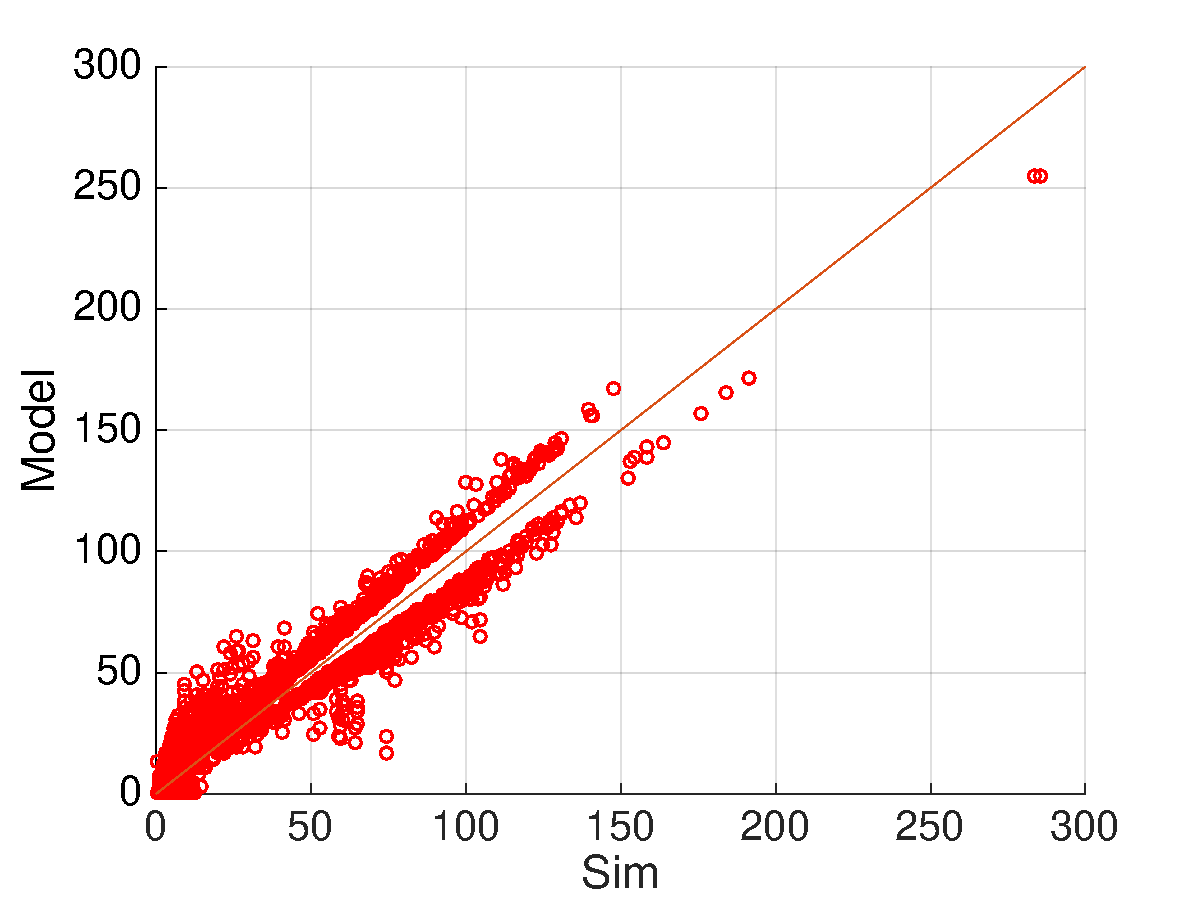
\includegraphics[width=0.33\textwidth]{figures/scatter_results-error-GPR5020-opti-all-sort_L0_1}}
%      \subfloat[Relative error $>=$ 0.2  \label{fig:delay-alpha-0}]{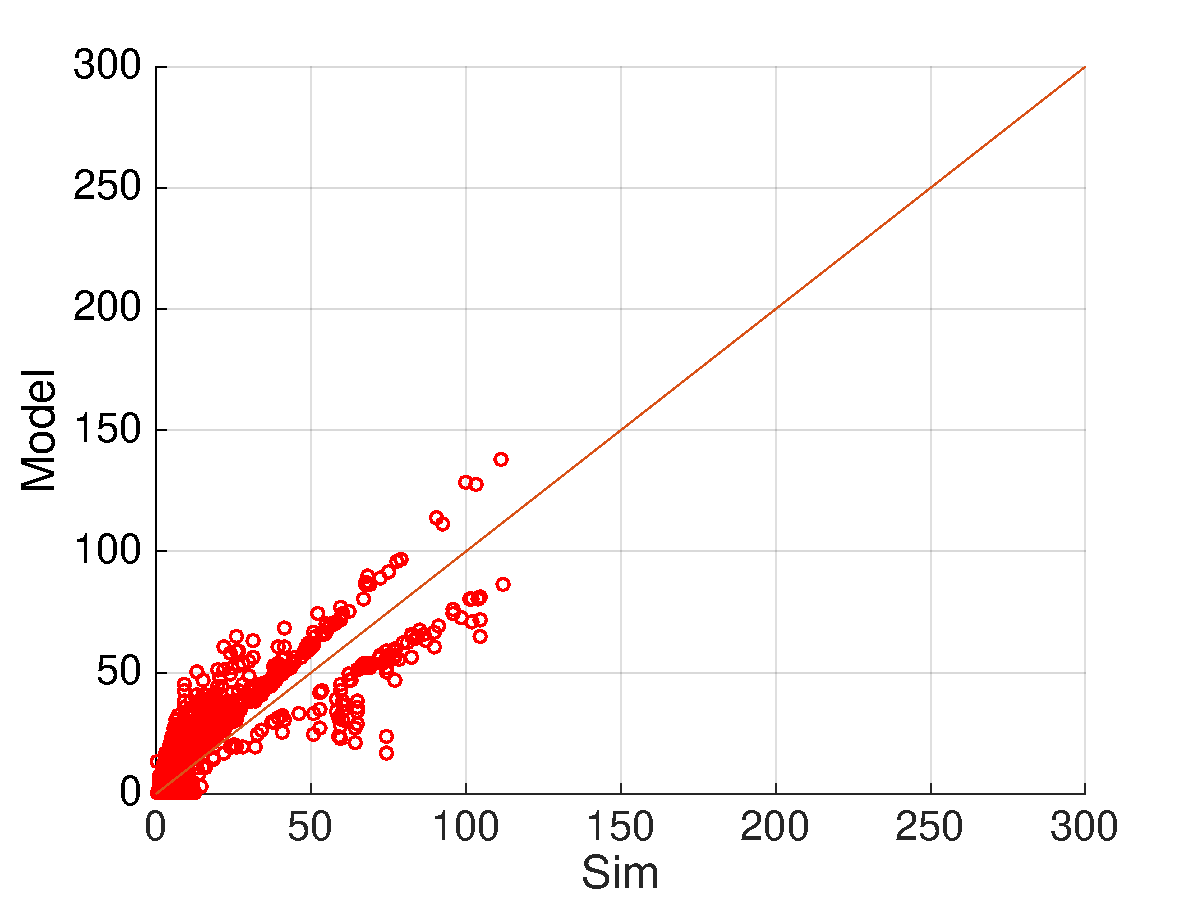
\includegraphics[width=0.33\textwidth]{figures/scatter_results-error-GPR5020-opti-all-sort_L0_2}}
%   \caption{Scatter plot. \label{fig:scatter-plot}}
% \end{figure*}

% \begin{figure*}[t]
%     \centering
%     \subfloat[Surrogate model prediction vs. simulation results \label{fig:scatter_all}]{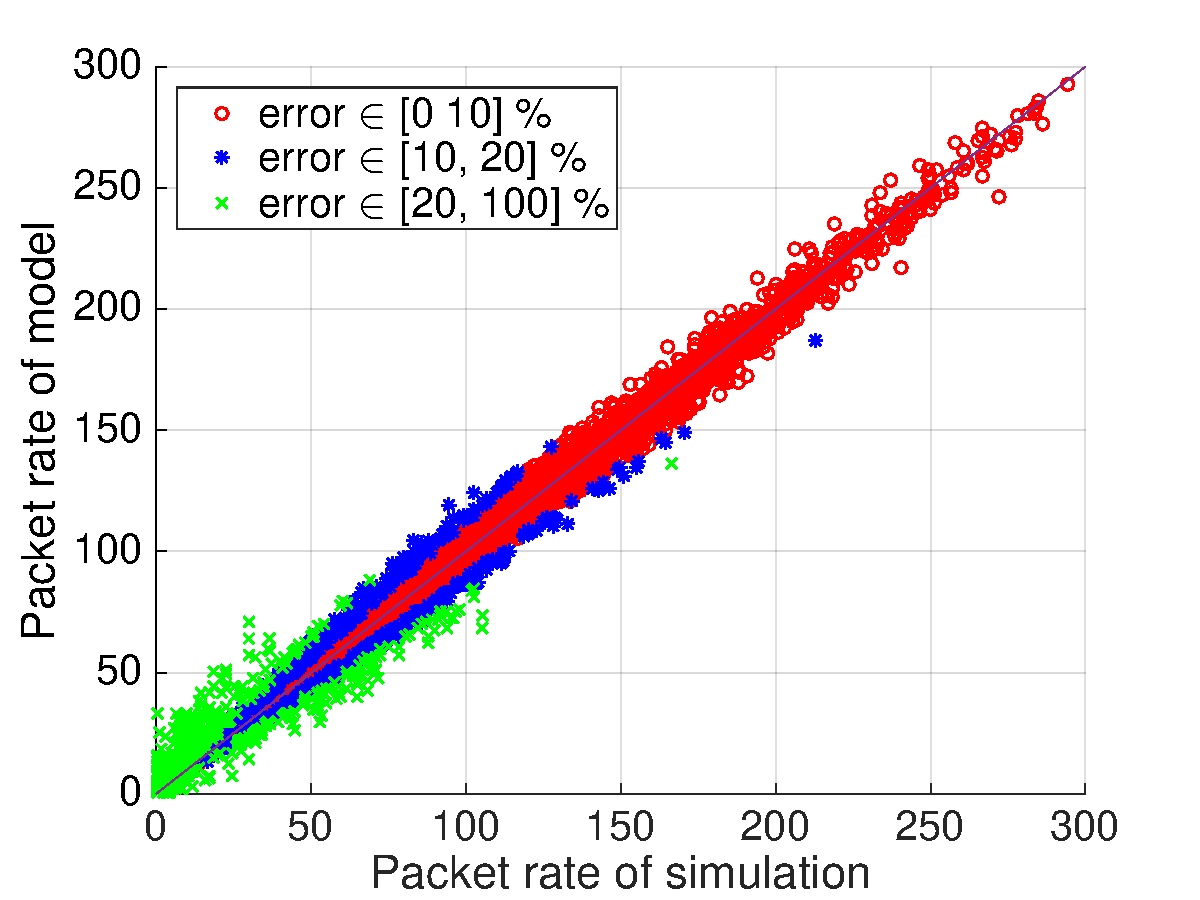
\includegraphics[width=0.45\textwidth]{figures/scatter_full}}
%     \subfloat[Relative error  \label{fig:full_design_error}]{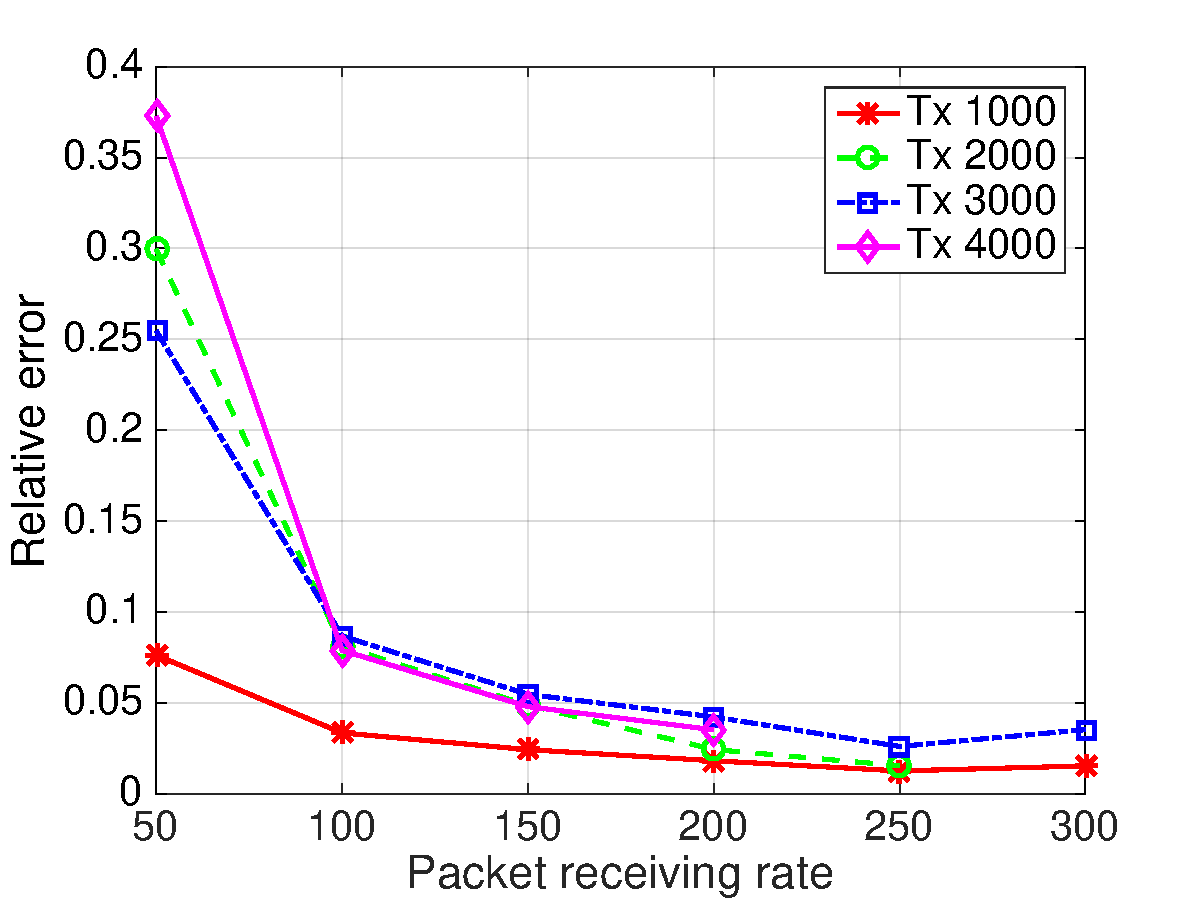
\includegraphics[width=0.45\textwidth]{figures/full_design_error}}
%   \caption{Comparison between the simulation results and surrogate model's prediction for the test data points, in terms of average packet receiving rate \label{fig:scatter-plot}}
% \end{figure*}


\begin{figure*}[t]
    \centering
    \subfloat[Surrogate model prediction vs. simulation results \label{fig:scatter_all}]{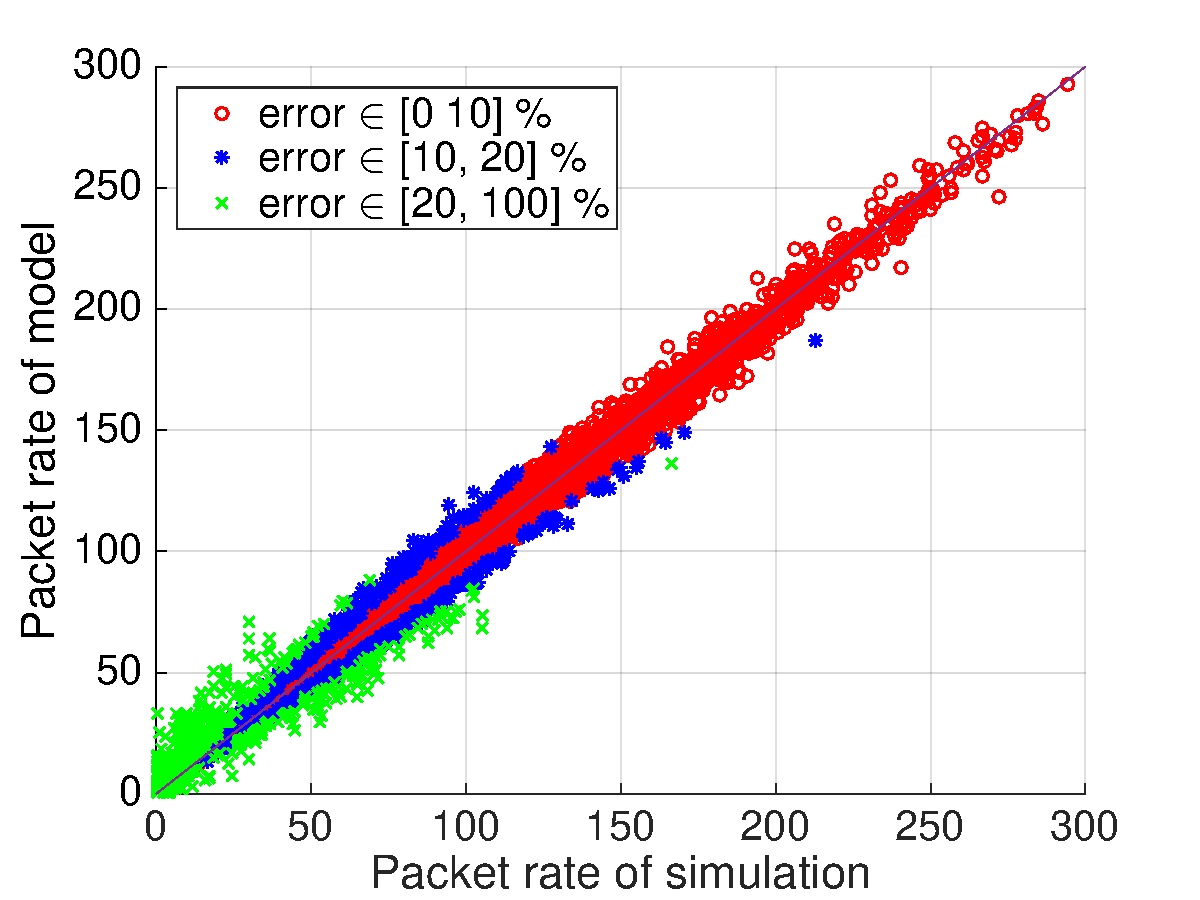
\includegraphics[width=0.33\textwidth]{figures/scatter_full}}
  %  \subfloat[Relative error for all packet receiving rate \label{fig:full_design_error}]{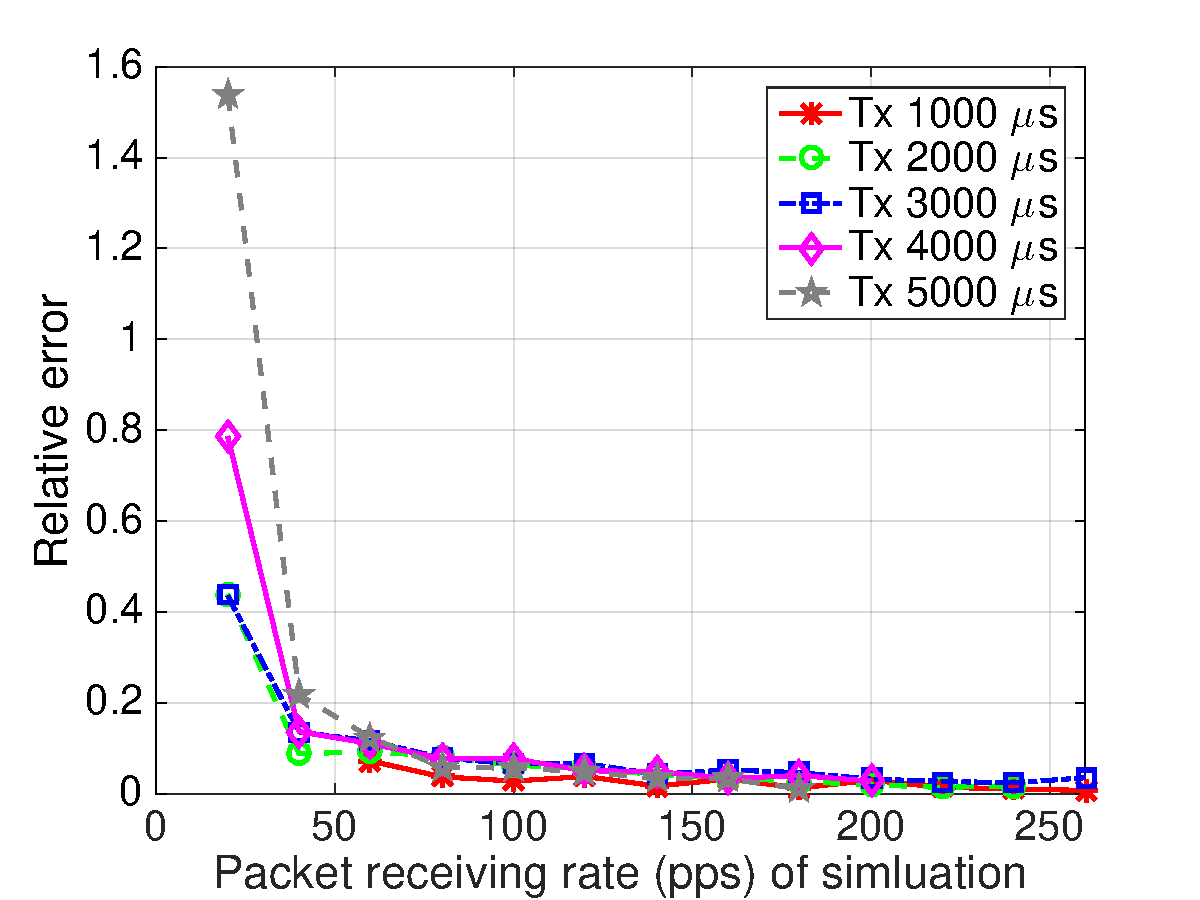
\includegraphics[width=0.33\textwidth]{figures/full_design_error_all}}
    \subfloat[Relative error for all packet receiving rate \label{fig:full_design_error}]{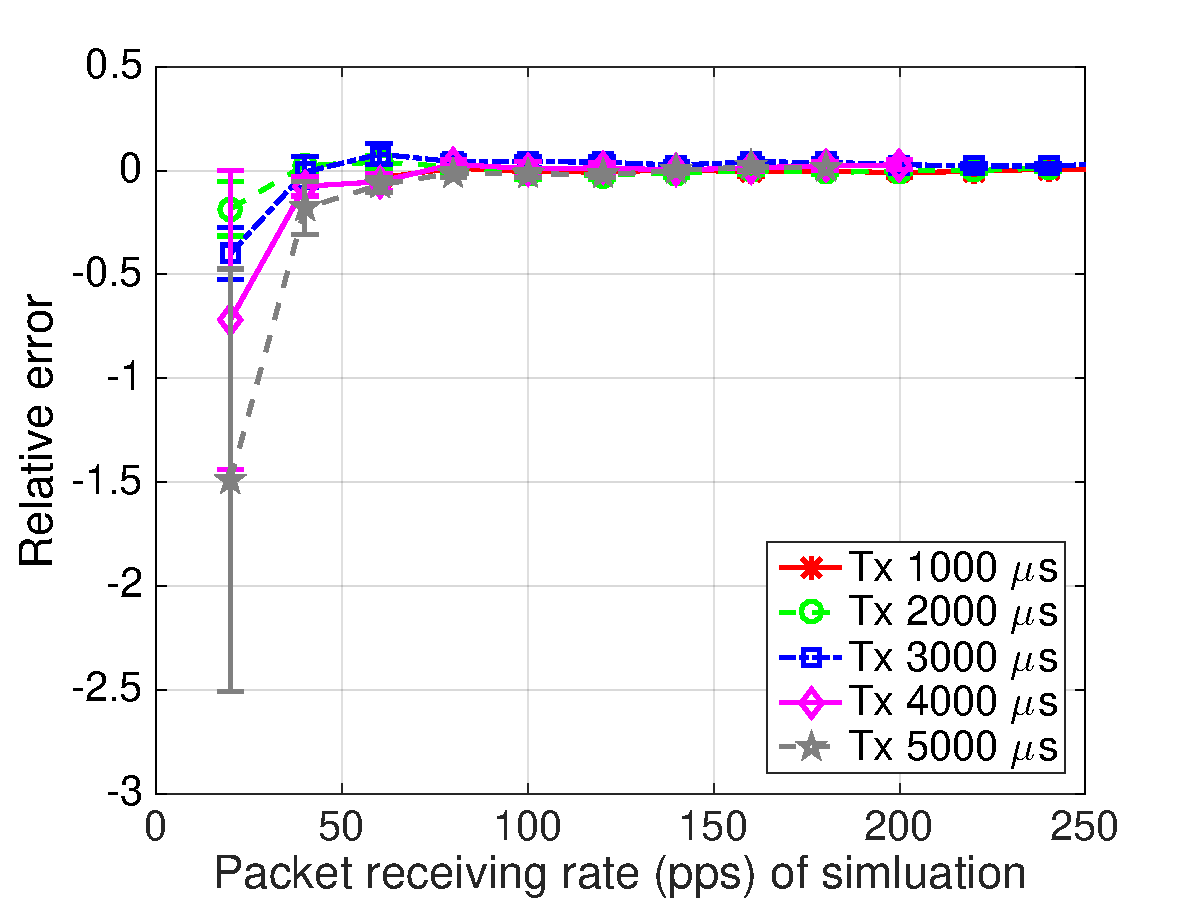
\includegraphics[width=0.33\textwidth]{figures/full_design_relative_error_all}}
    % \subfloat[Relative error for all packet receiving rate larger than 50 \gls{pps}. \label{fig:full_design_error}]{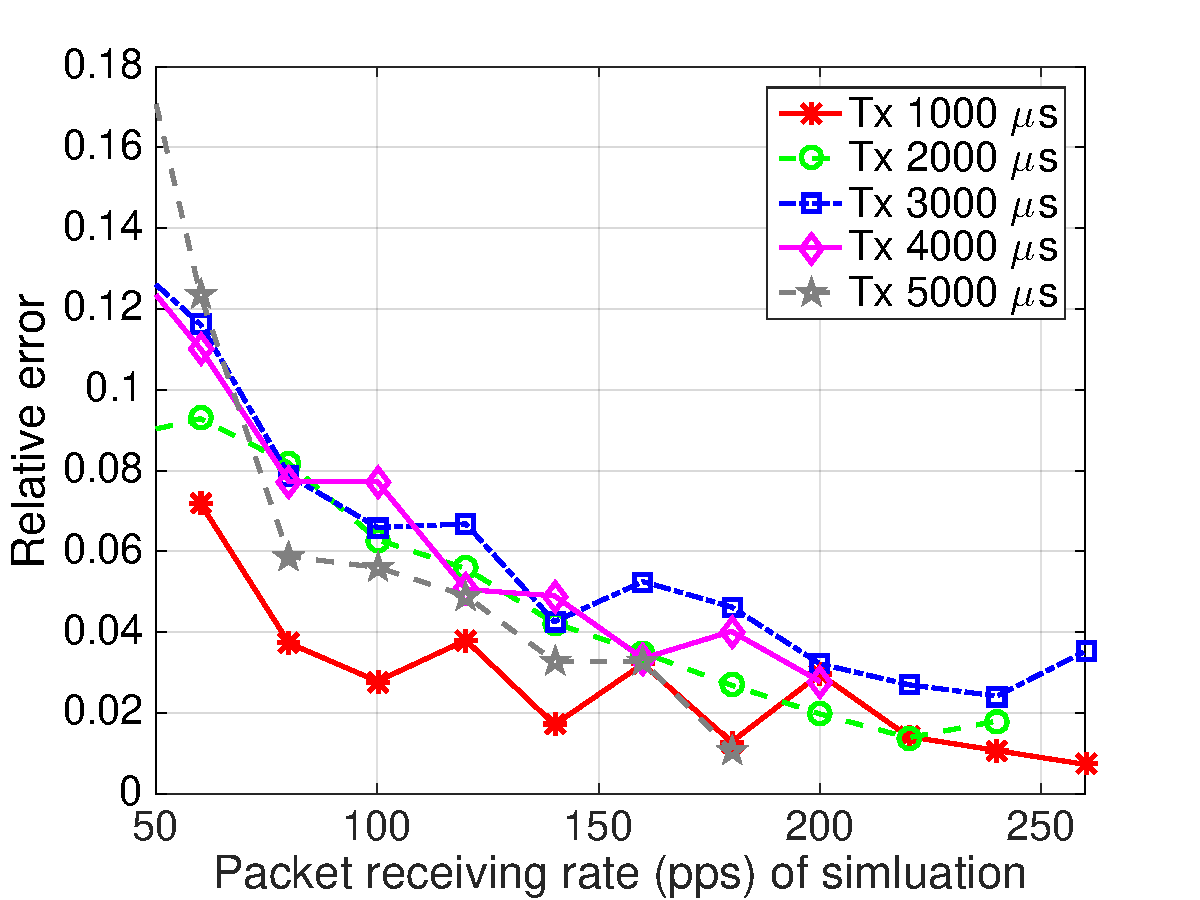
\includegraphics[width=0.33\textwidth]{figures/full_design_error_L50}}
      \subfloat[Relative error for all packet receiving rate larger than 60 \gls{pps}. \label{fig:full_design_error_L60}]{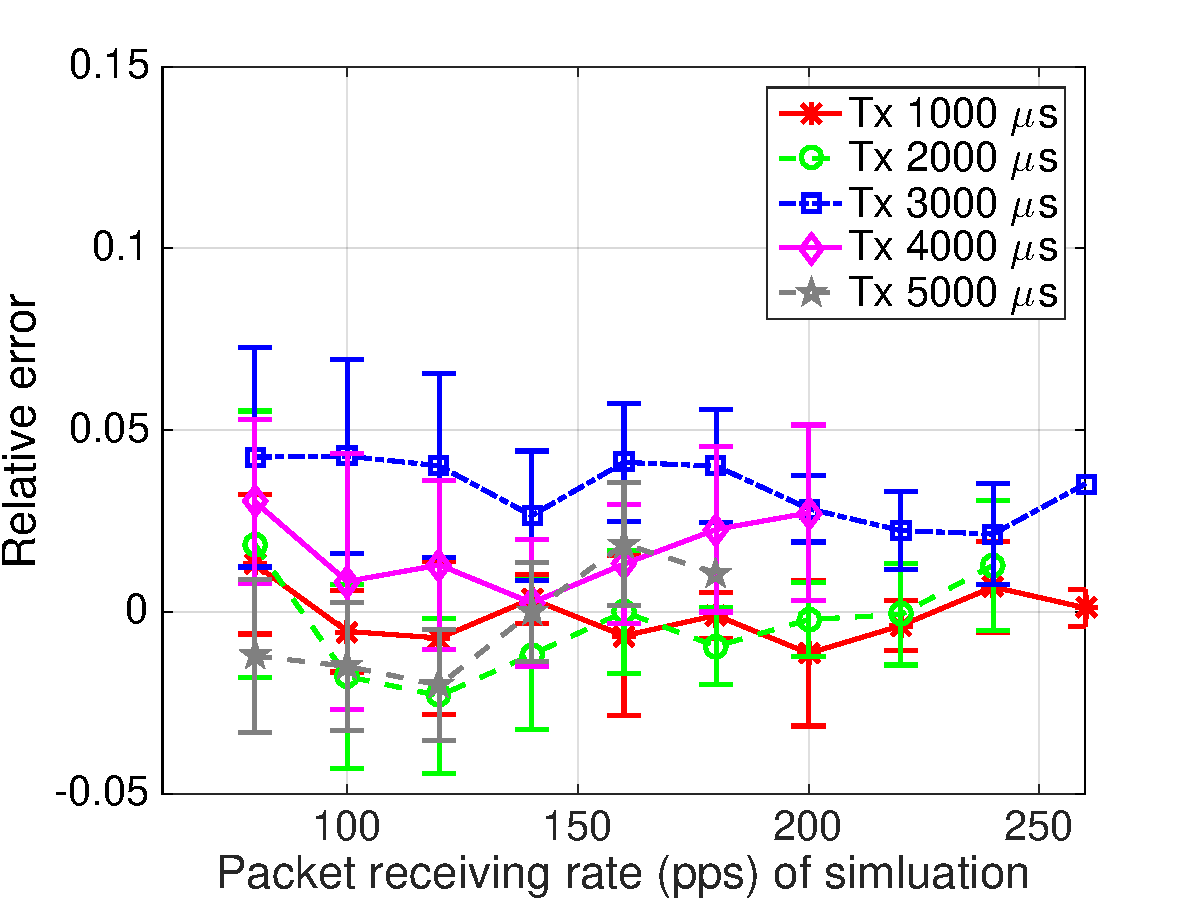
\includegraphics[width=0.33\textwidth]{figures/full_design_relative_error_all_L60}}
  \caption{Comparison between the simulation results and surrogate model's prediction for the test data points, in terms of average packet receiving rate \label{fig:scatter-plot}}
\end{figure*}

% \begin{figure*}[t]
%     \centering
%     \subfloat[Tx 1000 us  \label{fig:scatter_ana_tx1000}]{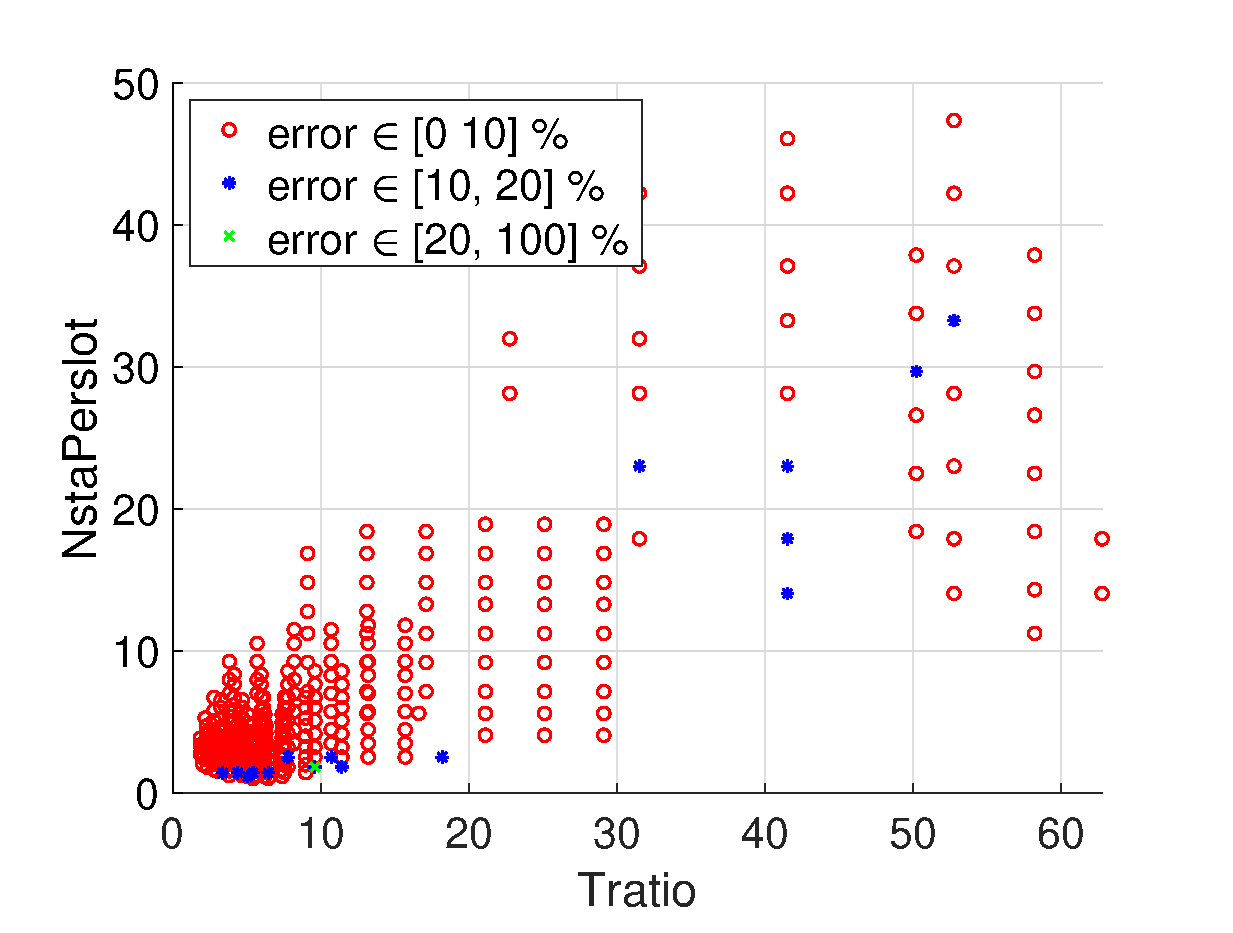
\includegraphics[width=0.33\textwidth]{figures/nstaPerSlot_Tratio_scatter_tx1000}}
%     \subfloat[Tx 3000 us \label{fig:scatter_ana_tx3000}]{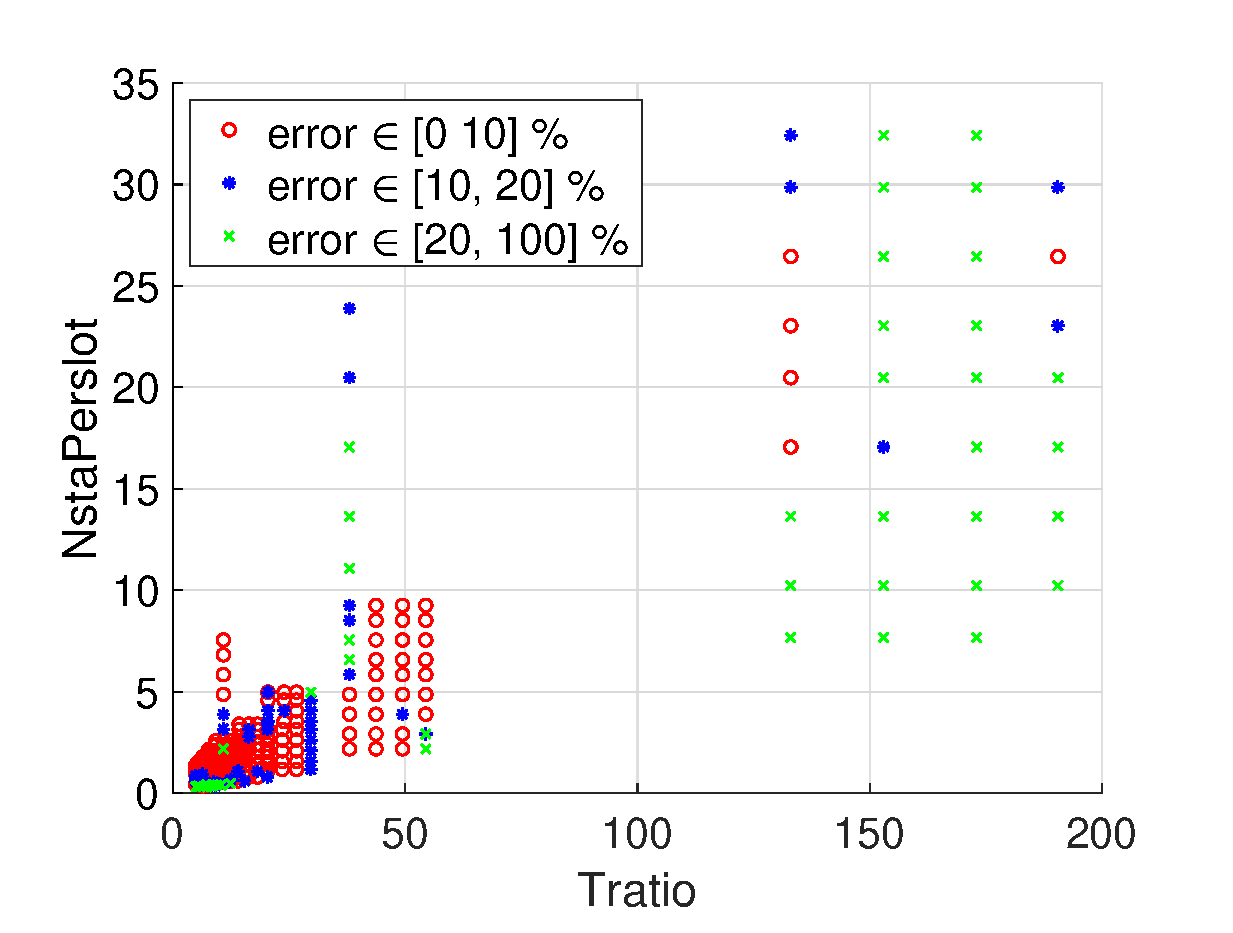
\includegraphics[width=0.33\textwidth]{figures/nstaPerSlot_Tratio_scatter_tx3000}}
%     \subfloat[Tx 4000 us \label{fig:scatter_ana_tx4000}]{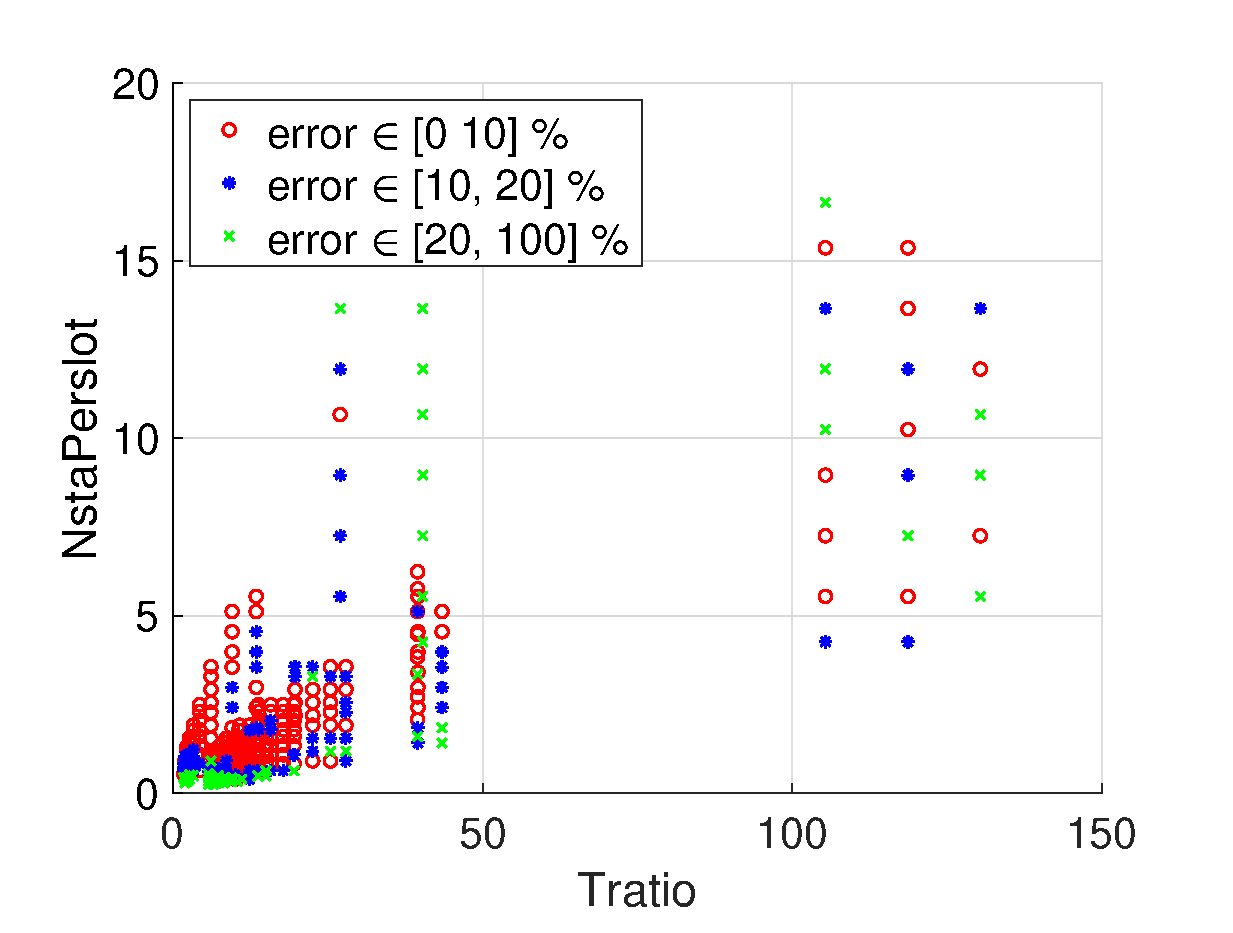
\includegraphics[width=0.33\textwidth]{figures/nstaPerSlot_Tratio_scatter_tx4000}}
%     %\subfloat[Full design space with various types of transmission time \label{fig:delay-alpha-0}]{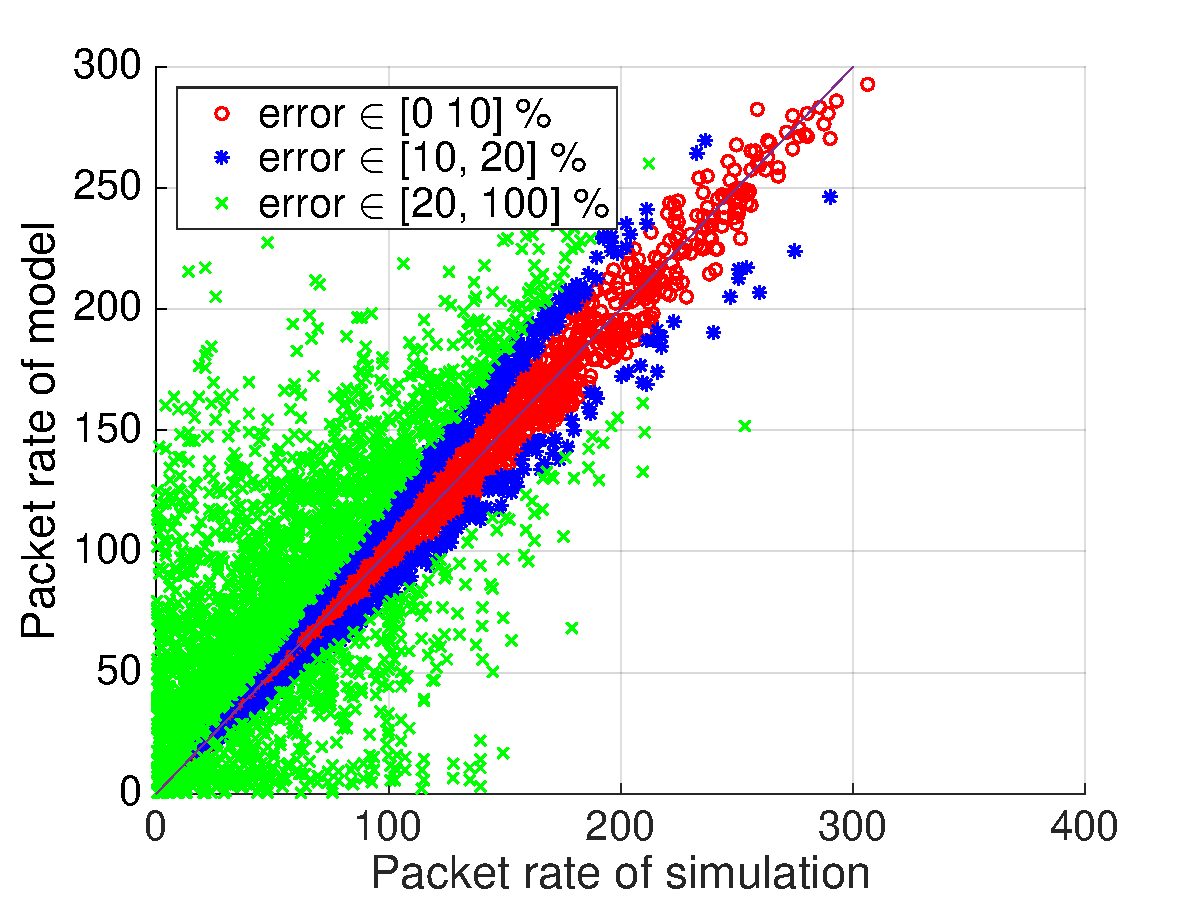
\includegraphics[width=0.33\textwidth]{figures/scatter_randomTx}}
%   \caption{Illustration of the relations among model accuracy and $n^{\alpha}_r$ and  $d^{\beta}_r$. \label{fig:scatter-plot-ana}}
% \end{figure*}




% \begin{figure}[t]
%     \centering
%     \subfloat[Color represents the transmission time (us)  \label{fig:delay-alpha-0}]{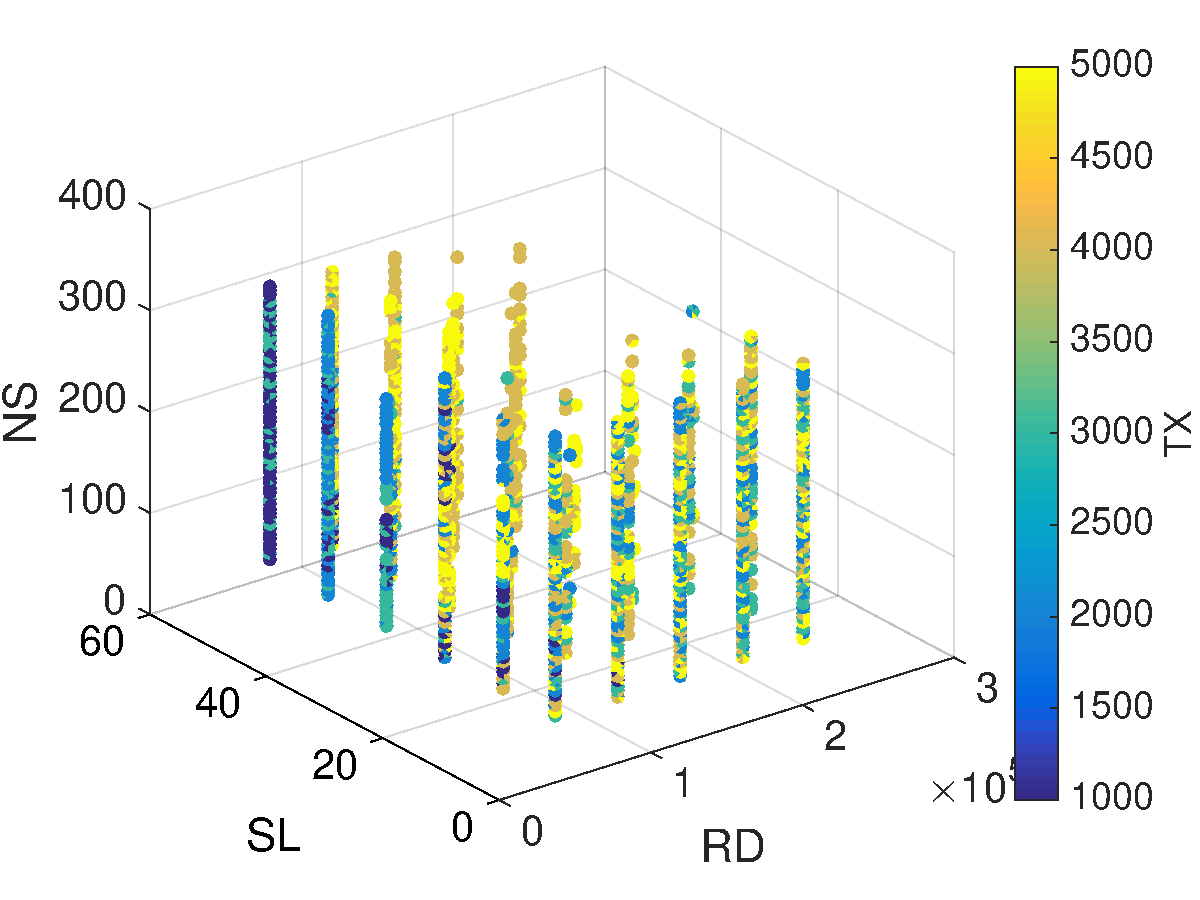
\includegraphics[width=0.8\columnwidth]{figures/scatter_results-error-GPR5020-opti-all-sort-3D-L0_1}} \\
%      \subfloat[Color represents the slot number  \label{fig:delay-alpha-0}]{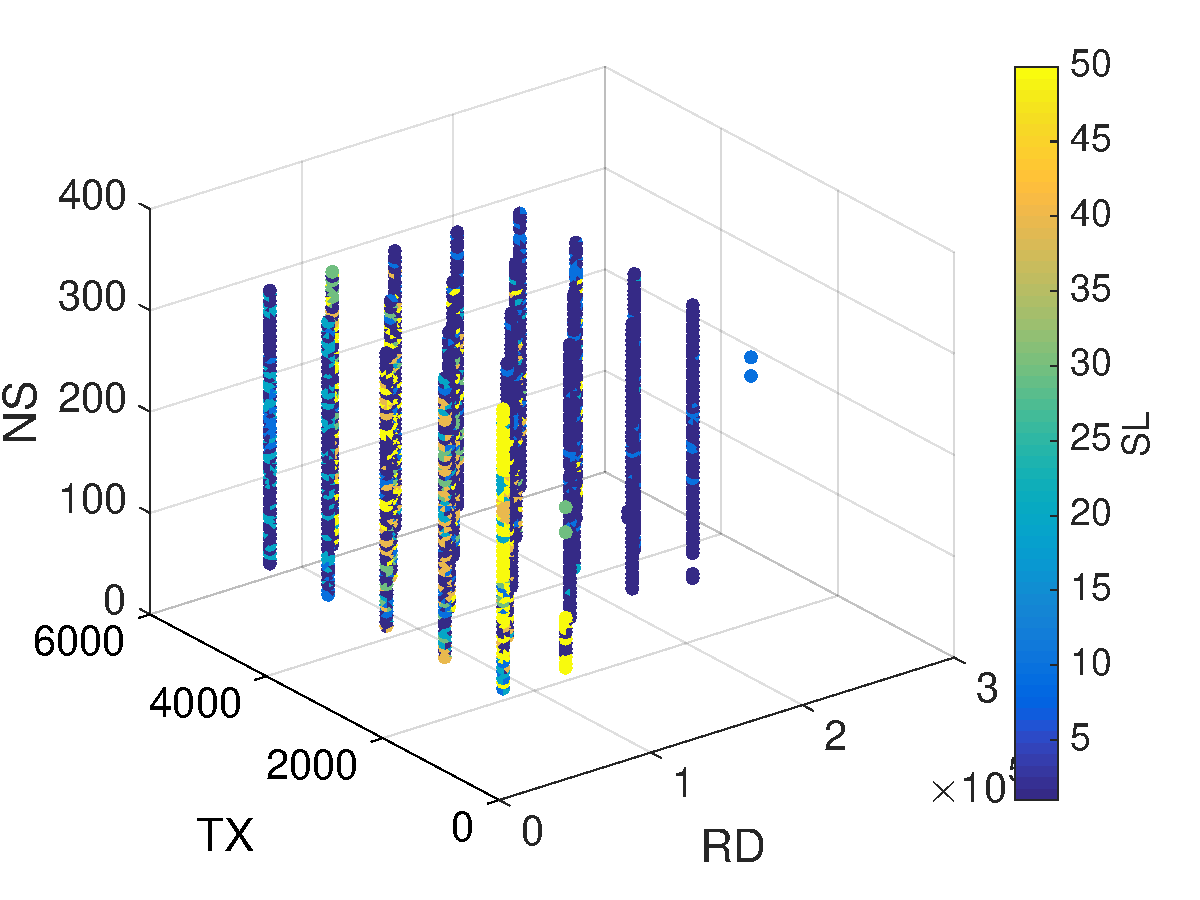
\includegraphics[width=0.8\columnwidth]{figures/scatter_results-error-GPR5020-opti-all-sort-3D-L0_1-angle}} 
%   \caption{3D Scatter plot for Relative error $>=$ 0.1. \label{fig:3d-Scatter-plot}}
% \end{figure}


% \begin{figure}[t]
%     \centering
% {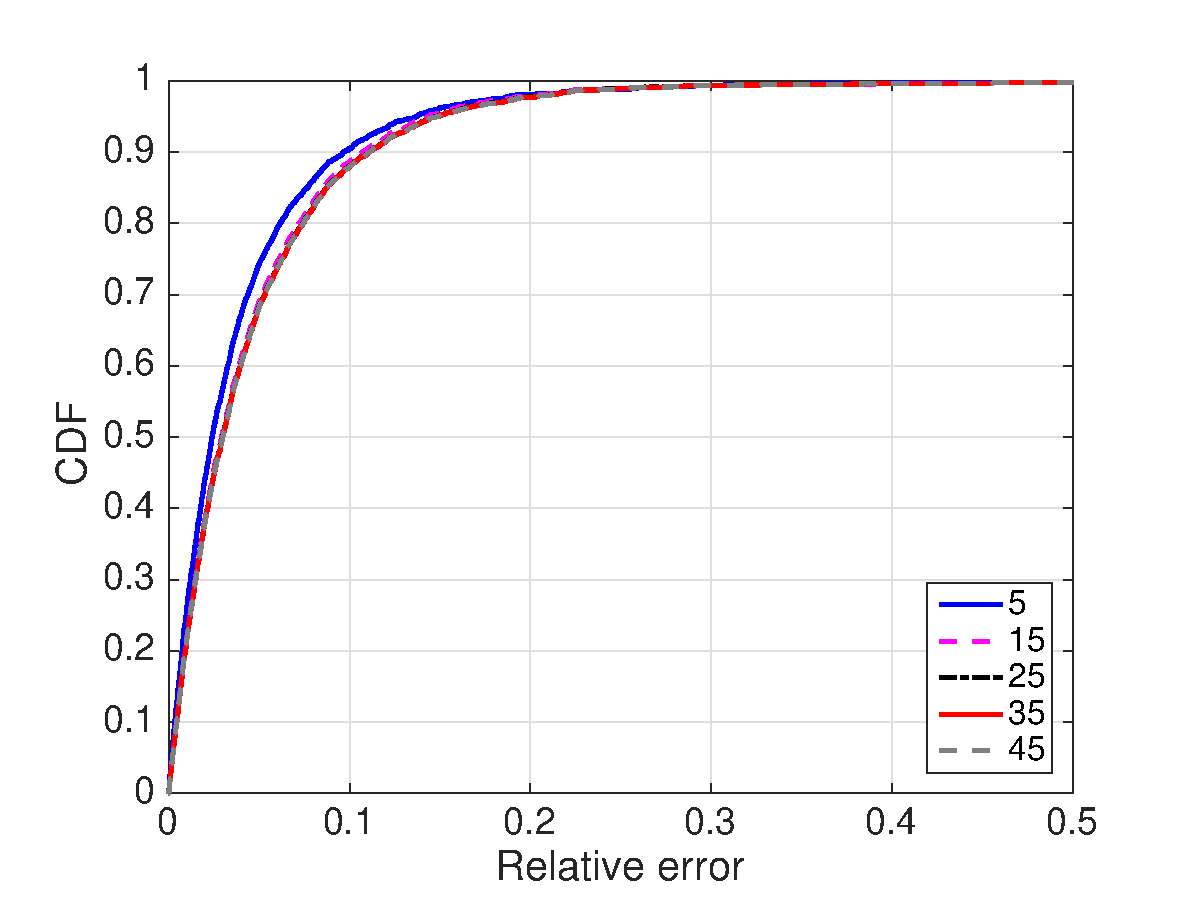
\includegraphics[width=0.8\columnwidth]{figures/cdf_all_ratio_NstaPslot_S50_Tratio_L1}}
%   \caption{Accuracy of \gls{gpr} regression model for full design space with different slot load ratio. \label{fig:cdf_constraint}}
% \end{figure}

\begin{figure}[t]
    \centering
%{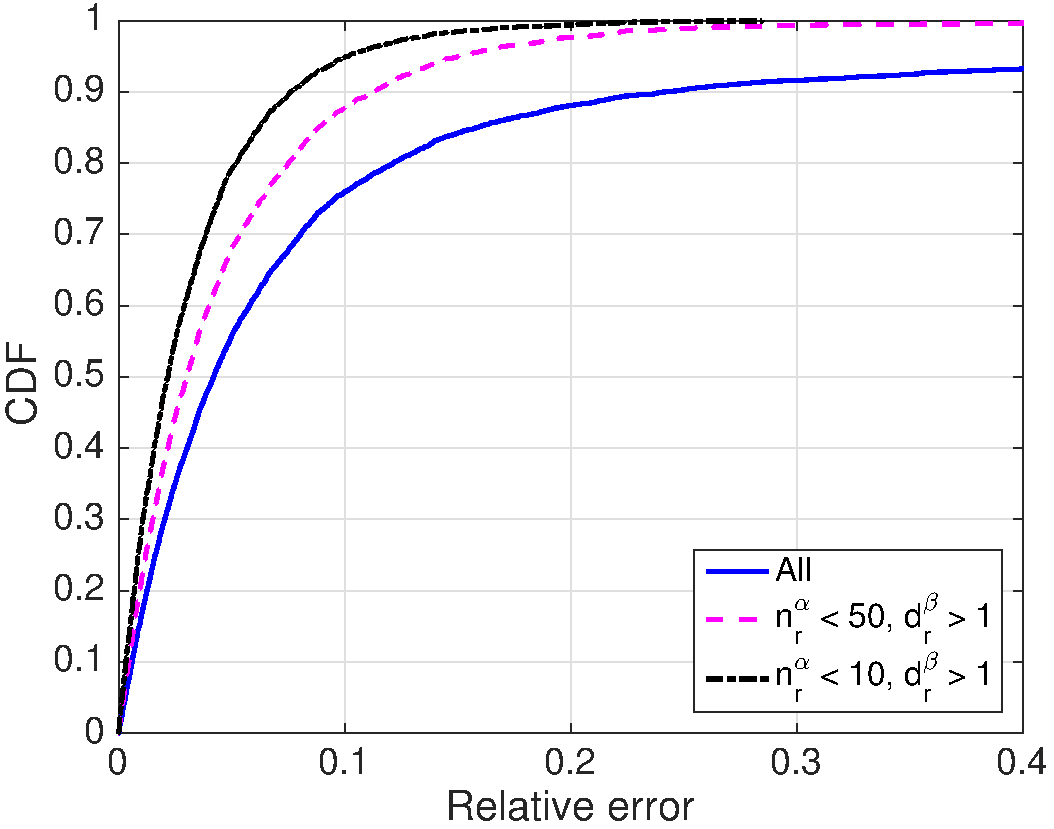
\includegraphics[width=0.8\columnwidth]{figures/full_constraint}}
%{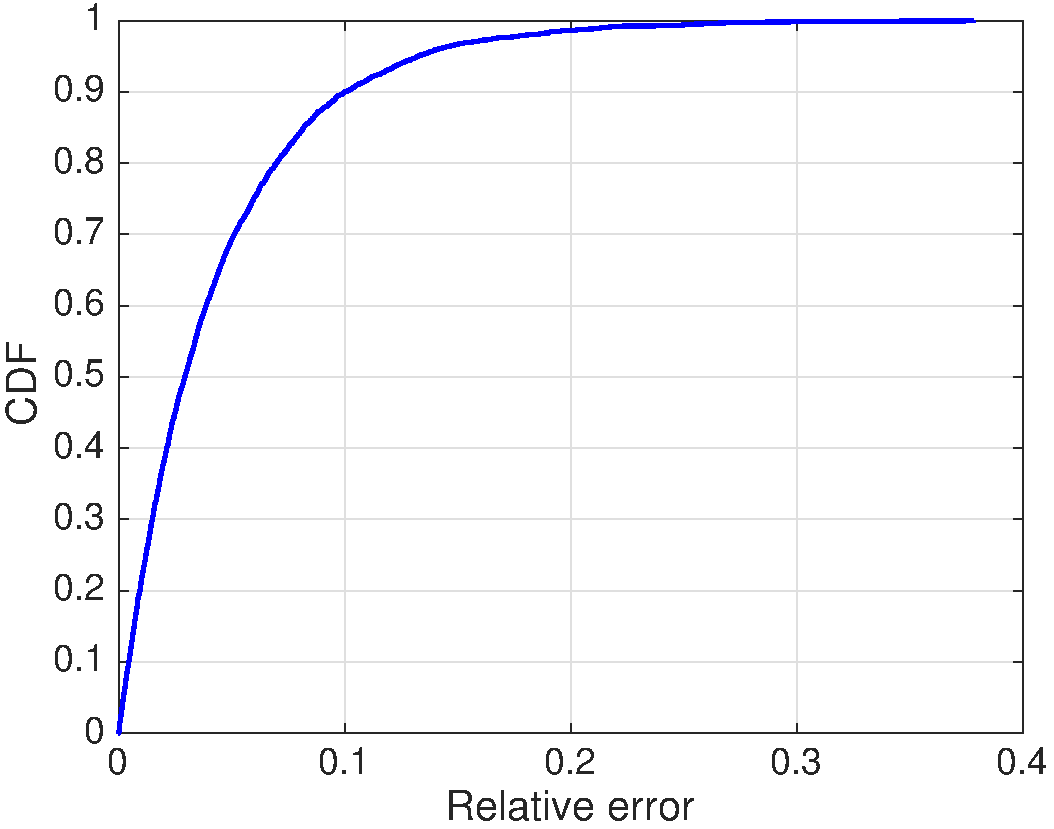
\includegraphics[width=0.8\columnwidth]{figures/full_constrain_L60}}
{\includegraphics[width=0.8\columnwidth]{figures/full_constrain_L60_PDR_08}}
  \caption{Accuracy of surrogate model using Kriging method for packet receiving rate larger than 60 and \gls{pdr} larger than 0.8 in full design space. \label{fig:cdf_constraint}}
\end{figure}




% \begin{figure}[t]
%     \centering
%     \subfloat[Relative error $<=$ 0.1  \label{fig:delay-alpha-0}]{\includegraphics[width=0.8\columnwidth]{figures/random_NstaPerSlot_Tratio_S01}} \\
%      \subfloat[Relative error $>$ 0.1 \label{fig:delay-alpha-0}]{\includegraphics[width=0.8\columnwidth]{figures/random_NstaPerSlot_Tratio_L01}} 
%   \caption{Distribution of station number per slot and xx for different Relative error \label{fig:3d-Scatter-plot}}
% \end{figure}


% \begin{figure}[t]
%     \centering
% {\includegraphics[width=0.8\columnwidth]{figures/cases_reduced}}
%   \caption{Accuracy of \gls{gpr} regression model for full and reduced design space. \label{fig:casess}}
% \end{figure}



% \begin{figure}[t]
%     \centering
% {\includegraphics[width=0.8\columnwidth]{figures/cases_randomTx}}
%   \caption{Accuracy of \gls{gpr} regression model for full design space with various types of transmission time. \label{fig:cases_randomTx}}
% \end{figure}


% \begin{figure}[t]
%     \centering
% {\includegraphics[width=0.8\columnwidth]{figures/sim-compare-rd204800-sl10}}
%   \caption{Comparison of simulation results for transmission time (2000 us) with different distance range of packet size range . \label{fig:tx_diff_compare}}
% \end{figure}



% \begin{figure}[t]
%     \centering
% {\includegraphics[width=0.8\columnwidth]{figures/same_diff}}
%   \caption{Accuracy of \gls{gpr} regression model for same and different MCS and packet size (reduced design space). \label{fig:cases_reduced}}
% \end{figure}

% \begin{figure*}[t]
%     \centering
%     \subfloat[same \label{fig:delay-alpha-0}]{\includegraphics[width=0.45\textwidth]{figures/same_sim_model_scatter}}
%     \subfloat[diff \label{fig:delay-alpha-0}]{\includegraphics[width=0.45\textwidth]{figures/diff_sim_model_scatter}}
%   \caption{Scatter plot. \label{fig:scatter-plot-tx}}
% \end{figure*}

% \begin{figure}[t]
%     \centering
% {\includegraphics[width=0.8\columnwidth]{figures/seed_sim_model_scatter}}
%   \caption{Comparison between simulation results using different seed . \label{fig:seed-comparison}}
% \end{figure}


% \begin{figure}[t]
%     \centering
% {\includegraphics[width=0.8\columnwidth]{figures/result-rd204800-pslot}}
%   \caption{comparison between model and simulation with * stations per slots. \label{fig:staPerSlot}}
% \end{figure}

In this section, we evaluate the \gls{raw} model accuracy for the reduced design space, in which the average transmission time consists of the coverage and packet size ranges used during the training process. 
%As the design space includes xx data points, it is extremely expensive to run all experiments. Therefore, 
6000 data points (called test data points) are randomly chosen for the evaluation of the model. To evaluate the accuracy of kriging model (with Matem 5/2) used in the model creation step, three additional regression models (i.e., linear regression, \gls{svm} and regression trees) are also created with the trained data points for comparison. The simulation results of the 6000 test data points are compared to the prediction of the models. 


% Figure \ref{fig:regress-models} depicts the probability that the relative error (i.e., ratio between absolute throughput error and simulation results) of the  models compared to simulation are equal to or less than a given relative error.

Figure \ref{fig:regress-models} depicts the \gls{cdf} of the absolute relative error, i.e., ratio between absolute error of the simulation results $S_r$ and model predication $P_r$ , and simulation results $S_r$, i.e., 
\begin{equation}
%\hat{f} (X) = \sum_{i=1}^{V} {a_i}{k(x, x_i)}
Abs. \thinspace relative \thinspace error = \frac{\abs{S_r - P_r} }{S_r} 
\end{equation}
It shows 76\% of the test data points has a relative error equal to or less than 0.1 for kriging model with Matem 5/2, while 30\%, 10\% and 44\% for the linear regression, \gls{svm}, regression tree models respectively. Similarly,  for kriging model, 88\% of the test data points result in  a relative error not larger than 0.2, the percentage declines to 53\%, 17\% and 65\% for the linear regression, \gls{svm} and regression tree models respectively. The results show the Kriging model has higher accuracy than the other three regression models. However, there are still some data points with high relative error and we will further investigate. 
%the model is not good enough to be directly applied to the \gls{raw} modeling problem. %\textcolor{red}{consider to remove the line of Kriging, Matem 3/2}.


To further explore the performance of the Kriging model, Figure \ref{fig:scatter-plot}  shows a scatterplot of the output of simulation and predication of the model.
%for the same test data points.
The line  $y=x$ represents the ideal case where the model can precisely predict the output of all data points without any errors. Points located near the line $y=x$ indicates that they can be accurately predicated by the model, and vice versa. The points are color-coded based on the relative errors, red means the relative error lower than 0.1, blue represent the relative error between 0.1 and 0.2, and green indicates the error larger than 0.2. Figure \ref{fig:scatter_all} reveals interesting characteristic of the created \gls{raw} model, the large error mainly exists for the small packet rates, which makes sense as a small absolute error leads to a large relative error. As the model is mainly used for \gls{raw} optimization, we are more interested in the large values, as these signify higher throughput and better performance. Most of the points with relative error between 0.1 and 0.2 have packet rate below 150, most of the relative error larger than 0.2 appear when the packet rate is below 100, large errors are especially concentrated at packet rates below 23. Figure \ref{fig:full_design_error} and \ref{fig:full_design_error_L60} respectively depicts, for all the data points and data points with packet receiving rate larger than 60, the average relative error and its 95\% confidence intervals as a function of the packet receiving rate with transmission time $1000$, $2000$, $3000$, $4000$ and $5000$ $\mu$s respectively. The relative error is defined as 
\begin{equation}
%\hat{f} (X) = \sum_{i=1}^{V} {a_i}{k(x, x_i)}
Relative \thinspace error = \frac{{S_r - P_r} }{S_r} 
\end{equation}
Similarly. it shows the large relative errors mainly exist for small packet receiving rate. When focus on the large packet receiving rate (i.e., larger than 60), the relative error only is between -0.045 and 0.075. Moreover, the relative error varies for points with different average transmission times, the smaller average transmission time results in less relative error than larger ones \todo{do more simulations, to make the results more clear}. The \gls{cdf} of the relative error for the Kriging model is updated with packet receiving rate larger than 60 and \gls{pdr} larger than 0.8, and depicted in Figure \ref{fig:cdf_constraint}. As it shows, for packet receiving rate larger than 60, about 90\% of the data points have a relative error equal to or less than 0.1, improving 18\%. If the data points is further filtered with \gls{pdr} larger than 0.8, about 98\% of the data points have a relative error less than 0.1, and 88\% for relative error less than 0.05.



% Moreover, the relative error varies for points with different average transmission times. Figure \ref{fig:full_design_error} depicts the relative error as a function of the packet receiving rate (simulation result) with transmission time $1000$, $2000$, $3000$, $4000$ and $5000$ $\mu$s respectively. Similar to figure  \ref{fig:scatter_all}, it shows the high relative error mainly exists for low packet receiving rate. Moreover, the results reveals the smaller average transmission time results in less relative error than larger average transmission. 


 
%  Compare to transmission time $4000$ \textit{us}, the transmission time $1000$ \textit{us} results in much less error, there is a few points with error between 10\% and 20\%, and errors beyond 20\% (\textcolor{red}{the figure needs to be replotted}). While transmission time $4000$ \textit{us} has the similar error distribution as figure \ref{fig:scatter_all}. In addition, for the same packet rate, transmission time $1000$ \textit{us} results in less error than $4000$ \textit{us} does. For example, it has much less points with error between 10\% and 20\% in the packet rate range [50, 150].


% Take $1000$ and $4000$ \textit{us} as an example, figure \ref{fig:scatter_tx1000} and \ref{fig:scatter_tx4000} depict the scatterplot for points with transmission time $1000$ and $4000$ \textit{us} respectively. Compare to transmission time $4000$ \textit{us}, the transmission time $1000$ \textit{us} results in much less error, there is a few points with error between 10\% and 20\%, and errors beyond 20\% (\textcolor{red}{the figure needs to be replotted}). While transmission time $4000$ \textit{us} has the similar error distribution as figure \ref{fig:scatter_all}. In addition, for the same packet rate, transmission time $1000$ \textit{us} results in less error than $4000$ \textit{us} does. For example, it has much less points with error between 10\% and 20\% in the packet rate range [50, 150].

In conclusion, based on the above results, we discover that, for the design space, the surrogate \gls{raw} model can accurately predict the output when the packet receiving rate is high, which is vital for the \gls{raw} model as it is commonly used for maximizing the packet receiving rate (equivalent to high throughput). In the next section, the model accuracy for the extrapolated design space will be evaluated.
%Therefore, the model can actually be applied to the \gls{raw} modeling problem if only the data points resulting in high packet receiving rate are considered from the model.

%Last but not least, the output (packet rate) of data point with high transmission time has higher variance.

% \textcolor{red}{Two question of figure \ref{fig:regress-models}:} \\
% \textcolor{red}{Should CDF of relative error be used or cross validation score?} \\
% \textcolor{red}{Should a random test data set or the training data set be used?} \\
%\item Measure accuracy in all cases, find weaknesses in the model. \\
 
 
%As the goal of \gls{raw} is to maximize the throughput (packet receiving rate) in dense scenarios with heavy traffic load, the \gls{raw} configurations that result in low packet rate can be excluded from the model, allowing the model to accurately predict the output of the given \gls{raw} configuration.
 
 %Let $NstaPSlot$ denote the number of stations per \gls{raw} slot, and $Tratio$ represent the ratio between \gls{raw} slot duration and transmission time.
 
% Figure \ref{fig:scatter-plot-ana} shows the scatterplot of the number of stations in one \gls{raw} slot ($N^{\alpha}_{r}$) and the ratio between \gls{raw} slot duration and transmission time ($N^{\beta}_r$), for different relative errors. As it reveals, for transmission times $3000$ and $4000$ \textit{us}, the larger errors mainly exist for \gls{raw} configuration in which either too many stations contend for the channel in one \gls{raw} slot or the \gls{raw} slot duration is too short to transmit one packet, resulting in low packet rate \textcolor{red}{(not depicted)}. Therefore, to accurately predict the output of a given \gls{raw} configuration, a constraint is added when applying the model, i.e., 
% \begin{equation} \label{eq:constraint}
% n^{\alpha}_r < \alpha \wedge d^{\beta}_r >= \beta
% \end{equation}

% Through analyzing the simulation results and model, we found out that the low packet rate are mainly caused by the inefficient \gls{raw} configurations, either too much stations contending the channel in one raw slot or the raw slot duration is too short to transmit one packet. 
%\item Go to more realistic cases at the end of this section, where the results are better. (for reduced and full design space, to compare the difference in performance) \\

% Therefore, the \gls{cdf} of the relative error for the Kriging model is updated with different $\alpha$ and $\beta$, and depicted in Figure \ref{fig:cdf_constraint}. As it shows, nearly 90\% of the data points have a relative error equal to or less than 0.1 for $\alpha = 50$ and $\beta = 1$. If $\alpha$ is further reduced to 10, the percentage goes up to 95\%. 





% Figure \ref{fig:casess} shows the accuracy of \gls{gpr} regression model under different cases. 
% The performance of model accuracy between reduced and full design space is compared. \\
% \textcolor{red}{what kind of data set should be used for comparison? \\
% \begin{enumerate}
% \item data set including points inside and outside of the reduced design space?
% \item or two different data set? one is inside, another one is outside.
% \end{enumerate}
%}

\subsection{Full design space experiments}

% \begin{figure*}[t]
%     \centering
%     \subfloat[tx1000 204800 \label{fig:tx_diff_tx1000}]{\includegraphics[width=0.45\textwidth]{figures/tx1000_204800}}
%     \subfloat[tx5000 204800 \label{fig:tx_diff_tx5000}]{\includegraphics[width=0.45\textwidth]{figures/tx5000_204800}}
%   \caption{Comparison of simulation results for transmission time (2000 us) with different distance range of packet size range. \label{fig:tx_diff_compare}}
% \end{figure*}

%  One of the input parameters used by the \gls{raw} modeling, \textit{average transmission time}, is actually represented by two parameters of the 802.11ah network, i.e., distance between stations and \gls{ap}, and packet size of the stations. In the modeling process, for each average transmission time, the network are configured with a fixed distance range and packet size. However, there are a large number of distance and packet size range that can lead to the same average transmission time. 
 
 The results in previous section have demonstrated that, for the high values, the built model has high accuracy on predicting the output for the design space. In this section, we further explore the performance of the model for the extrapolated design space. In the extrapolated design space, a data point with average transmission time Tx, consists of different coverage and packet size ranges than the one used during the training.
 
 
 \begin{figure}[t]
    \centering
%{\includegraphics[width=0.8\columnwidth]{figures/Extend_constraint}}
%{\includegraphics[width=0.8\columnwidth]{figures/Extend_constraint_08}}
{\includegraphics[width=0.8\columnwidth]{figures/Extend_constraint_09}}
  \caption{Accuracy of surrogate model using Kriging method for packet receiving rate larger than 60 and \gls{pdr} larger than 0.8 in extrapolated design space. \label{fig:cdf_constraint_extended}}
\end{figure}
 
The 6000 test data points used in previous section are again simulated. However, unlike previous simulations for the design space, for a data point with average transmission time $T_x$, the simulator randomly selects a  coverage and packet size range which can result in the average transmission time $T_x$. The simulation results are compared to the output of the built models, as shown in Figure \ref{fig:cdf_constraint_extended}. The results shows, compare to the design space, the model accuracy is much decreased,  both for all data points or for data points with packet receiving rate larger than 60. The lower model accuracy for the extrapolated design space is not surprising. In the modeling process, for each average transmission time, the network is configured with a fixed distance range and packet size. While in the extrapolated design space, for the same average transmission time, the network could could be configured with other distance  and packet size ranges. Therefore, model accuracy is sacrificed in order to speed up the training process. However, as discussed in Section \ref{subsubsec:txselection}, the model is mainly used for optimization, we are more interested in large values and high \gls{pdr}. By only take into account the data points with packet receiving rate larger than 60 and \gls{pdr} lager than 0.8, the model accuracy for the extrapolated design space is significantly improved. Around 85\% of the data points have relative error less than 0.1. 

% It shows, compare to the limited design space, the extrapolated design space results in more error in terms of model accuracy. 
% Even under the constraint $n^{\alpha}_r < 10 \wedge d^{\beta}_r >= 1$, the model accuracy is still not satisfying. Around 60\% of data points have relative error less than 10\%. The number goes up to 78\% for a relative error less than 20\%. The lower model accuracy for the extrapolated design space is not surprising. In the modeling process, for each average transmission time, the network is configured with a fixed distance range and packet size. However, in the extrapolated design space, for the same average transmission time, the network could could be configured with other distance  and packet size ranges. Therefore, model accuracy is sacrificed in order to speed up the training process. This aligns with our discovery in Section \ref{subsubsec:txselection}, which also indicates high model accuracy can still be achieved for the scenarios that we are interested in, \todo{explain the scenarios}. 
 
%  In order to make the trained model more applicable to the extrapolated design space, we first explore the performance difference of a variety of distance and packet size range leading to the same average transmission time. For each data point, 10 different distance and packet size range are randomly selected and simulated. Take average transmission time  $1000$ and $5000$ us as an example, figure \ref{fig:tx_diff_compare} shows, the packet receiving rate as a function of station number for \gls{raw} duration $204800$ \textit{us} and slot number $10$. The lines represent the 10 different iterations. The result shows that the same packet rate is achieved until a certain number of stations, then discrepancy among the packet rates of different distance and packet size ranges starts to appear. Moreover, the breaking points where the discrepancy occurs depends on the average transmission time. As figure \ref{fig:tx_diff_tx1000} shows, the packet rate start to vary when station number is 260, while the performance difference is triggered by much less stations (around 45) fro transmission time $5000$ \textit{us}.  With a given slot number and \gls{raw} duration, station number determines the traffic load of the \gls{raw} slot. Therefore, figure \ref{fig:tx_diff_compare} indicates that, the performance discrepancy is caused by the  high traffic load $L_r$:  \\
% \begin{equation}
% \mathcal{L}_{r} = \frac {n_r \times TXOP} {d_r \times \mathcal{T}_s}.
% \end{equation}
% Where $TXOP$ indicate the TXOP time including data packet transmission time ($T_x$), a SIFS (160 us) and the ACK transmission time (1000 us), $\mathcal{T}_s$ represents the packet sending interval of a station. The minimal slot traffic load which can cause performance discrepancy is denoted as $\mathcal{L}_r^max$, in order to apply the model to the extended design space, the slot traffic load needs to be no larger than the $\mathcal{L}_r^max$.
% For transmission time $1000$ and $5000$ \textit{us}, the  $\mathcal{L}_r^max$ are \textcolor{red}{xx} and \textcolor{red}{xx}, respectively. %As the DIFS and backoff time is not taken into account, 


To further evaluate the model accuracy, We randomly choose 500 design points for each load ratio (i.e., 0.4, 0.6, 0.8, 1.0), consisting of 5 different average transmission time (i.e., 1000, 2000, 3000, 4000 and 5000 $\mu$s). During simulation, for each design point, the network is configured with a randomly coverage and packet size range, while satisfying the average transmission time $T_x$. Each simulation runs for 10 times. For the evaluation, we only take into account the data points with packet receiving rate larger than 60 and \gls{pdr} lager than 0.8. The relative error of each design point between the simulation results and the surrogate model is calculated. For each average transmission time, the relative error is averaged among data points with the same packet receiving rate and slot load ratio respectively. Furthermore, the relative error is averaged among all iterations. The results are depicted in figure \ref{fig:results-extended-prate} and \ref{fig:results-extended-load} respectively, including  average relative error and its 95\% confidence intervals. 
%with the variability of result over these iterations quantified using the standard deviation (SD).


% Under the constraint indicated in equation \ref{eq:constraint} with $\alpha=10$ and $\beta=1$, the relative error of each design point between the simulation results and the surrogate model is calculated. For each average transmission time, the relative error is averaged among data points with the same packet receiving rate and slot load ratio respectively. Furthermore, the relative error is averaged among all iterations, as depicted in figure \ref{fig:results-extended-prate}   and \ref{fig:results-extended-load} respectively . 

The results show, for the extrapolated design space, the surrogate model is able to accurately predict the network performance. As depicted in Figure \ref{fig:results-extended-prate}, the relative error is between -0.1 and 0.1 for most data points. Especially for average transmission time 1000 $\mu$s, the relative error is only between -0.003 and 0.02. The similar results are obtained in Figure \ref{fig:results-extended-load} as well. For \gls{raw} slot load ratio no more than 0.4, the relative error is between -0.042 to 0.038. With larger \gls{raw} slot ratio, for average transmission time between 1000 and 4000 $\mu$s, the relative error is between -0.005 to 0.125.  For average transmission time 5000 $\mu$s, the relative error is between -0.03 and 0.08.

% the relative error increases with higher average transmission time. Moreover, the small packet receiving rate (less than or equal to 50) results in high relative error, while 
% By excluding the data points with the packet receiving rate less than or equal to 50, figure \ref{fig:results-extended-load} further reveals the model accuracy varies on the \gls{raw} slot load. For average transmission time 1000 us, the relative error is only 0.38\% for slot load ratio 0.4, and increase to 7.6\% for overloaded traffic (i.e., slot load ratio 1.6\%). Average transmission time 2000, 3000 and 4000 us have similar relative errors \textcolor{red}{from slot load ratio 0.4 and 1.0} (i.e., non saturated traffic conditions), ranging from 3.6\% to 14.1\%. While for average transmission time 5000 us, the relative error is already 23.4\% for slot load ratio 1, and increases to 53.5\% for slot load ratio 1.6.



% The results show, for the extrapolated design space, the surrogate model is able to accurately predict the network performance. As depicted in Figure \ref{fig:results-extended-prate}, the relative error increases with higher average transmission time. Moreover, the small packet receiving rate (less than or equal to 50) results in high relative error, while small relative error is obtained for larger packet receiving rates. 
% By excluding the data points with the packet receiving rate less than or equal to 50, figure \ref{fig:results-extended-load} further reveals the model accuracy varies on the \gls{raw} slot load. For average transmission time 1000 us, the relative error is only 0.38\% for slot load ratio 0.4, and increase to 7.6\% for overloaded traffic (i.e., slot load ratio 1.6\%). Average transmission time 2000, 3000 and 4000 us have similar relative errors \textcolor{red}{from slot load ratio 0.4 and 1.0} (i.e., non saturated traffic conditions), ranging from 3.6\% to 14.1\%. While for average transmission time 5000 us, the relative error is already 23.4\% for slot load ratio 1, and increases to 53.5\% for slot load ratio 1.6.

%\textcolor{red}{analysis of optimal raw duration and slot number for a given station number and average transmission time.}


% \begin{figure}[t]
%     \centering
% {\includegraphics[width=0.8\columnwidth]{figures/1_50_tx3000.pdf}}
%   \caption{Performance for extended design space with different slot load ratio and average transmission time. \label{fig:results-extended}}
% \end{figure}



% \begin{figure*}[t]
%     \centering
%     \subfloat[Tx 1000-4000 us  \label{fig:tx_diff_tx1000}]{\includegraphics[width=0.45\textwidth]{figures/1_50_error_toTx4000.pdf}}
%     \subfloat[Tx 4000-5000 us  \label{fig:tx_diff_tx5000}]{\includegraphics[width=0.45\textwidth]{figures/1_50_error_toTx5000.pdf}}
%   \caption{Performance for extrapolated design space with different slot load ratio and average transmission time. \textcolor{red}{to be merged}   \label{fig:results-extended-load}}
%   % not fliter out small output
% \end{figure*}

 \begin{figure}[t]
    \centering
%{\includegraphics[width=0.8\columnwidth]{figures/tx_result_load_all_yxlim}}
{\includegraphics[width=0.8\columnwidth]{figures/avg_result_Prate_tx_extend_08}}
  \caption{Performance for extrapolated design space with different packet receiving rate and average transmission time. \label{fig:results-extended-prate}}
  % new load ratio, from 2-8
\end{figure}


 \begin{figure}[t]
    \centering
%{\includegraphics[width=0.8\columnwidth]{figures/1_50_error_fliter}}
{\includegraphics[width=0.8\columnwidth]{figures/avg_result_load_tx_extended_08}}
  \caption{Performance for extrapolated design space with different slot load ratio and average transmission time. \label{fig:results-extended-load}}
  % new load ratio, from 2-8, fliter out small output
\end{figure}


% \begin{figure*}[t]
%     \centering
%     \subfloat[Tx 1000-3000 us  \label{fig:tx_diff_tx1000}]{\includegraphics[width=0.45\textwidth]{figures/tx_1_3000.pdf}}
%     \subfloat[Tx 4000-5000 us  \label{fig:tx_diff_tx5000}]{\includegraphics[width=0.45\textwidth]{figures/tx_1_4_5000.pdf}}
%   \caption{Performance for extrapolated design space with different slot load ratio and average transmission time. \label{fig:results-extended}}
% \end{figure*}






%As the ns-3 based 802.11ah simulator provides a quite realistic simulation environment, in which the propagation loss, capture effect are considered, the distribution of distance (Equivalent to MCS) and packet size imposes an impact on the channel contention and thus affect the packet rate.


% The figure \ref{fig:cases_reduced} compares the model accuracy for both reduced and full design space under realistic cases. A random test including xx data points belonging to the full design space was simulated and the results are compared to the  models of reduced and full design space. When compared to the reduced design space, for the data points outside of the design space, we choose the output of the closest data points inside the reduced design space as its approximation. Therefore, in fact, the model for the reduced design space (figure \ref{fig:cases_reduced}) is a Interpolation.

% \item Same MCS and packet size
% \begin{itemize}
% \item CDF of relative error.
% \item Scatter plot
% \item Compare model and simulation results.
% \end{itemize}

% \item Different MCS and packet size
% \begin{itemize}
% \item Comparison of regression models
% \item CDF of relative error, graphs with different constraints can be shown.
% \item Compare model and simulation results.
% %\item Compare model and simulation results, number of staitons per slot.
% \end{itemize}

%\item plot ''accuracy = Tsim (RDm, SLm) / Tsim (RDs, SLs)" 
%\textcolor{red}{The test data set needs to be large enough, otherwise the accuracy could be much larger than 1.}

%\item throughput comparison
%\item analysis of optimal raw duration and slot number for a given station number and average transmission time.
%\end{itemize}



% \subsection{Exploring optimal \gls{raw} configuration}

% %\textcolor{red}{analysis of optimal raw duration and slot number for a given station number and average transmission time.}

% We evaluate the scenarios in which stations are randomly located around the \gls{ap} with distance no more than 500 meters, and have packet size between 64 and 512 bytes. The average transmission time of such networks are around 2000 us. Figures \ref{fig:result-rd} compares the surrogate model and simulation results under different stations number, slot number and \gls{raw} duration. The lines represents the simulation results, and the the dots represent the  model prediction. As it shows, the simulation results and the model predictions are quite close in most cases, and most importantly, always have the same trend. As it shows, the large \gls{raw} duration normally leads to higher packet rate, which is straightforward as there is more airtime for packet transmission. While too long \gls{raw} duration is a waste of airtime, as stations not belonging to the \gls{raw} group can not access the channel. The appropriate \gls{raw} duration should be just long enough for transmitting all the packets. For a given \gls{raw} duration, too many station could degrade the performance as too much collision occurs.
% It turns out a large number of \gls{raw} slot often leads to better performance, especially for large scale networks.

% % A better way to assess and apply the model is needed based on the following observations.
% % \begin{itemize}
% % \item The simulation results fluctuates with station number.
% % \item The simulation results and model have the same trend, but their actual values could be different.
% % \item Under average transmission time 2000 us, the optimal configuration (i.e., slot number) for a given station number and \gls{raw} duration are same for both model and simulation results. 
% % \end{itemize}

% % Figures \ref{fig:result-slot} 
% % compares model and simulations results with fixed average transmission time duration under different stations number, slot number and \gls{raw} duration.

% % A better way to assess and apply the model is needed based on the following observations.
% % \begin{itemize}
% % \item The simulation results fluctuates with station number, especially for the large distance range (i.e., 0~400 m and 0~500 meters).
% % \item The simulation results and model have the same trend.
% % \item The simulation results and model are close until a certain point (throughput/station number).
% % \item The optimal configuration (i.e., slot number) for a given station number and \gls{raw} duration are same for both model and simulation results. 
% % \end{itemize}

% % \textbf{Although the absolute output of the model and simulation does not match, they have the same trend, which is crucial in the selection of optimal \gls{raw} configuration under a given station number and average transmission time. especially for the scenarios whose distance and packet size range are different from the trained scenarios.}

% % The difference between model and results with 0-100 meters and slot 10/20, 0-300 m and slot 10, is caused by the average transmission time distribution. Due to the non cross slot boundary transmission features, packet has different chance to transmit during its own slot. 




% \begin{figure*}[t]
%     \centering
%     \subfloat[rd = 122880 us  \label{fig:delay-alpha-0}]{\includegraphics[width=0.33\textwidth]{figures/result-rd122880}}
%     \subfloat[rd = 163840 us \label{fig:delay-alpha-0}]{\includegraphics[width=0.33\textwidth]{figures/result-rd163840}}
%      \subfloat[rd = 204800 us \label{fig:delay-alpha-0}]{\includegraphics[width=0.33\textwidth]{figures/result-rd204800}}
%   \caption{Comparison between model and simulations results with fixed average transmission time (2000 us) under different stations number, slot number and \gls{raw} duration.  \label{fig:result-rd}}
% \end{figure*}


% % \begin{figure*}[t]
% %     \centering
% %     \subfloat[ 0-100 m \label{fig:delay-alpha-0}]{\includegraphics[width=0.33\textwidth]{figures/result-rd204800-range100}}
% %     \subfloat[ 0-300 m \label{fig:delay-alpha-0}]{\includegraphics[width=0.33\textwidth]{figures/result-rd204800-range300}}
% %      \subfloat[0-400 m \label{fig:delay-alpha-0}]{\includegraphics[width=0.33\textwidth]{figures/result-rd204800-range400}}
% %   \caption{Comparison between model and simulations results with fixed \gls{raw} duration (204800 us) under different stations number, slot number, distance range (transmission time).   \label{fig:result-range}}
% % \end{figure*}

% % \begin{figure*}[t]
% %     \centering
% %     \subfloat[ rd = 163840 us, 0-400 m \label{fig:delay-alpha-0}]{\includegraphics[width=0.45\textwidth]{figures/NstaPSlot-result-rd163840-range400}}
% %      \subfloat[ rd = 204800 us, 0-500 m \label{fig:delay-alpha-0}]{\includegraphics[width=0.45\textwidth]{figures/NstaPSlot-result-rd204800-range500}}
% %   \caption{Comparison between model and simulations results under different stations number, number of stations per slot, distance range.   \label{fig:result-slot}}
% % \end{figure*}

% % \begin{figure*}[t]
% %     \centering
% %     \subfloat[ 0-300 m \label{fig:delay-alpha-0}]{\includegraphics[width=0.45\textwidth]{figures/NstaPSlot-Thr-result-rd163840-range400}}
% %      \subfloat[ 0-100 m \label{fig:delay-alpha-0}]{\includegraphics[width=0.45\textwidth]{figures/NstaPSlot-Thr-result-rd204800-range500}}
% %   \caption{Comparison between model and simulations results with fixed \gls{raw} duration under different stations number, slot number, distance range.   \label{fig:result-slot-throughput}}
% % \end{figure*}



% % There are two ways to interpret the results.

% % The first one is, model can accurately predicts the output for practical scenarios, i.e., \gls{raw} duration is at least one/two times larger than average transmission time (one for trained transmission time, two for any transmission time composition), and no more than 10 stations assigned per slot. The downside is, some \gls{raw} configuration whose output can be very well  predicted are excluded from the practical scenarios". Figures like Figure \ref{fig:result-rd} and \ref{fig:result-range} can not be shown. One more question is also aroused, does the practical scenarios" includes the optimal \gls{raw} configuration for any given station number and transmission time. 

% % Figures/table needed:
% % \begin{itemize}
% % \item large relative error only exist for small output (option, only suitable for the trained scenarios, this can be caused by the applied machine learning model(kriging model in this case). This figure can be used to reveal/present the drawback(?) of the kriging model.   (Note:the reduced design space and full design space have quite same performance.)
% % \item scatter plot, highlight the \gls{raw} configuration that result in high relative error, and leads to the 
% % \item figures for constrained \gls{raw} configuration, including both design space reduced, full design space. \\
% % \textcolor{red}{figure \ref{fig:result-rd}, \ref{fig:result-range} can not be used due to the constraint, but results are actually quite good. There are two reasons, first, the constraints excludes some \gls{raw} configuration which has good performance, second, the results can still be good in some case even when the accuracy" is not high (figure \ref{fig:result-rd} has relative error 0.1 for 70\% data points.)}
% % \item  simulation results comparison between trained and untrained scenarios.
% % \item  Accuracy of untrained scenarios with refined constraints. 
% % \end{itemize}

% % Another option is, do not look at the absolute output of the model and simulation, but focus on the trend, they offer the same optimal \gls{raw} configuration.









\section{CONCLUSION AND FUTURE WORK \label{sec:conclusion}}

\textbf{Next steps or things need to do now}
\begin{enumerate}
\item retrain the model, split the transmission time into packet size range [Ps, Pe] and distance range [Ds, De]. \\
Quite complex to design the input for training, extrapolate the model, and  validate. Experiment design, the selection of range [s, e], and step size for both distance and packet size range. the step size. Output extrapolate (validation), for test scenarios that cross the two ranges [s, e], how to extrapolate the model and compare to simulation results?
\item retrain the model, add the standard deviation of the transmission time into the input parameters, which distribution should the transmission time should follow? How to design the step size? \\
\item Change the input parameters of the training. The input parameters [raw duration, slot number, station number] can be substituted by [slot duration, number of stations per slot]. \\
\textcolor{red}{This approach is not feasible, obviously, for a fixed number of station per slot, the outputs(throughput)} varies as the other input parameters (for example, the station number) changes. as illustrated in figure \ref{fig:result-rd} and figure \ref{fig:result-range}. Apparently, the station number determines the maximal output the network can achieve, and should not be removed from the input parameters list. 
\end{enumerate}



% The very first letter is a 2 line initial drop letter followed
% by the rest of the first word in caps.
% 
% form to use if the first word consists of a single letter:
% \IEEEPARstart{A}{demo} file is ....
% 
% form to use if you need the single drop letter followed by
% normal text (unknown if ever used by the IEEE):
% \IEEEPARstart{A}{}demo file is ....
% 
% Some journals put the first two words in caps:
% \IEEEPARstart{T}{his demo} file is ....
% 
% Here we have the typical use of a "T" for an initial drop letter
% and "HIS" in caps to complete the first word.
%\IEEEPARstart{T}{his} demo file is intended to serve as a ``starter file''
%for IEEE journal papers produced under \LaTeX\ using
%IEEEtran.cls version 1.8b and later.
%% You must have at least 2 lines in the paragraph with the drop letter
%% (should never be an issue)
%I wish you the best of success.
%
%\hfill mds
% 
%\hfill August 26, 2015

%\subsection{Subsection Heading Here}
%Subsection text here.

% needed in second column of first page if using \IEEEpubid
%\IEEEpubidadjcol

%\subsubsection{Subsubsection Heading Here}
%Subsubsection text here.


% An example of a floating figure using the graphicx package.
% Note that \label must occur AFTER (or within) \caption.
% For figures, \caption should occur after the \includegraphics.
% Note that IEEEtran v1.7 and later has special internal code that
% is designed to preserve the operation of \label within \caption
% even when the captionsoff option is in effect. However, because
% of issues like this, it may be the safest practice to put all your
% \label just after \caption rather than within \caption{}.
%
% Reminder: the "draftcls" or "draftclsnofoot", not "draft", class
% option should be used if it is desired that the figures are to be
% displayed while in draft mode.
%
%\begin{figure}[!t]
%\centering
%\includegraphics[width=2.5in]{myfigure}
% where an .eps filename suffix will be assumed under latex, 
% and a .pdf suffix will be assumed for pdflatex; or what has been declared
% via \DeclareGraphicsExtensions.
%\caption{Simulation results for the network.}
%\label{fig_sim}
%\end{figure}

% Note that the IEEE typically puts floats only at the top, even when this
% results in a large percentage of a column being occupied by floats.


% An example of a double column floating figure using two subfigures.
% (The subfig.sty package must be loaded for this to work.)
% The subfigure \label commands are set within each subfloat command,
% and the \label for the overall figure must come after \caption.
% \hfil is used as a separator to get equal spacing.
% Watch out that the combined width of all the subfigures on a 
% line do not exceed the text width or a line break will occur.
%
%\begin{figure*}[!t]
%\centering
%\subfloat[Case I]{\includegraphics[width=2.5in]{box}%
%\label{fig_first_case}}
%\hfil
%\subfloat[Case II]{\includegraphics[width=2.5in]{box}%
%\label{fig_second_case}}
%\caption{Simulation results for the network.}
%\label{fig_sim}
%\end{figure*}
%
% Note that often IEEE papers with subfigures do not employ subfigure
% captions (using the optional argument to \subfloat[]), but instead will
% reference/describe all of them (a), (b), etc., within the main caption.
% Be aware that for subfig.sty to generate the (a), (b), etc., subfigure
% labels, the optional argument to \subfloat must be present. If a
% subcaption is not desired, just leave its contents blank,
% e.g., \subfloat[].


% An example of a floating table. Note that, for IEEE style tables, the
% \caption command should come BEFORE the table and, given that table
% captions serve much like titles, are usually capitalized except for words
% such as a, an, and, as, at, but, by, for, in, nor, of, on, or, the, to
% and up, which are usually not capitalized unless they are the first or
% last word of the caption. Table text will default to \footnotesize as
% the IEEE normally uses this smaller font for tables.
% The \label must come after \caption as always.
%
%\begin{table}[!t]
%% increase table row spacing, adjust to taste
%\renewcommand{\arraystretch}{1.3}
% if using array.sty, it might be a good idea to tweak the value of
% \extrarowheight as needed to properly center the text within the cells
%\caption{An Example of a Table}
%\label{table_example}
%\centering
%% Some packages, such as MDW tools, offer better commands for making tables
%% than the plain LaTeX2e tabular which is used here.
%\begin{tabular}{|c||c|}
%\hline
%One & Two\\
%\hline
%Three & Four\\
%\hline
%\end{tabular}
%\end{table}


% Note that the IEEE does not put floats in the very first column
% - or typically anywhere on the first page for that matter. Also,
% in-text middle ("here") positioning is typically not used, but it
% is allowed and encouraged for Computer Society conferences (but
% not Computer Society journals). Most IEEE journals/conferences use
% top floats exclusively. 
% Note that, LaTeX2e, unlike IEEE journals/conferences, places
% footnotes above bottom floats. This can be corrected via the
% \fnbelowfloat command of the stfloats package.










% if have a single appendix:
%\appendix[Proof of the Zonklar Equations]
% or
%\appendix  % for no appendix heading
% do not use \section anymore after \appendix, only \section*
% is possibly needed

% use appendices with more than one appendix
% then use \section to start each appendix
% you must declare a \section before using any
% \subsection or using \label (\appendices by itself
% starts a section numbered zero.)
%

%
%\appendices
%\section{Proof of the First Zonklar Equation}
%Appendix one text goes here.
%
%% you can choose not to have a title for an appendix
%% if you want by leaving the argument blank
%\section{}
%Appendix two text goes here.


% use section* for acknowledgment
\section*{Acknowledgment}
The authors would like to thank...


%\bibliographystyle{abbrv}
\bibliographystyle{IEEEtran}
\bibliography{references.bib}


% Can use something like this to put references on a page
% by themselves when using endfloat and the captionsoff option.
% \ifCLASSOPTIONcaptionsoff
%   \newpage
% \fi



% trigger a \newpage just before the given reference
% number - used to balance the columns on the last page
% adjust value as needed - may need to be readjusted if
% the document is modified later
%\IEEEtriggeratref{8}
% The "triggered" command can be changed if desired:
%\IEEEtriggercmd{\enlargethispage{-5in}}

% references section

% can use a bibliography generated by BibTeX as a .bbl file
% BibTeX documentation can be easily obtained at:
% http://mirror.ctan.org/biblio/bibtex/contrib/doc/
% The IEEEtran BibTeX style support page is at:
% http://www.michaelshell.org/tex/ieeetran/bibtex/
%\bibliographystyle{IEEEtran}
% argument is your BibTeX string definitions and bibliography database(s)
%\bibliography{IEEEabrv,../bib/paper}
%
% <OR> manually copy in the resultant .bbl file
% set second argument of \begin to the number of references
% (used to reserve space for the reference number labels box)
%\begin{thebibliography}{1}
%
%\bibitem{IEEEhowto:kopka}
%H.~Kopka and P.~W. Daly, \emph{A Guide to \LaTeX}, 3rd~ed.\hskip 1em plus
%  0.5em minus 0.4em\relax Harlow, England: Addison-Wesley, 1999.
%
%\end{thebibliography}

% biography section
% 
% If you have an EPS/PDF photo (graphicx package needed) extra braces are
% needed around the contents of the optional argument to biography to prevent
% the LaTeX parser from getting confused when it sees the complicated
% \includegraphics command within an optional argument. (You could create
% your own custom macro containing the \includegraphics command to make things
% simpler here.)
%\begin{IEEEbiography}[{\includegraphics[width=1in,height=1.25in,clip,keepaspectratio]{mshell}}]{Michael Shell}
% or if you just want to reserve a space for a photo:

%\begin{IEEEbiography}{Michael Shell}
%Biography text here.
%\end{IEEEbiography}

% if you will not have a photo at all:
%\begin{IEEEbiographynophoto}{John Doe}
%Biography text here.
%\end{IEEEbiographynophoto}

% insert where needed to balance the two columns on the last page with
% biographies
%\newpage

%\begin{IEEEbiographynophoto}{Jane Doe}
%Biography text here.
%\end{IEEEbiographynophoto}

% You can push biographies down or up by placing
% a \vfill before or after them. The appropriate
% use of \vfill depends on what kind of text is
% on the last page and whether or not the columns
% are being equalized.

%\vfill

% Can be used to pull up biographies so that the bottom of the last one
% is flush with the other column.
%\enlargethispage{-5in}



% that's all folks
\end{document}


